\documentclass[letterpaper,12pt,oneside]{book}
%%
%%  Template de mémoire de maîtrise ou thèse de doctorat.
%%  Normalement, il n'est pas nécessaire de modifier ce document
%%  sauf pour changer les noms des fichiers à inclure.
%%
%%  Version: 2014-10-28
%%
%%  Accepte les caractères accentués dans le document (UTF-8).
\usepackage[utf8]{inputenc}
%%
%% Support pour l'anglais et le français (français par défaut).
%\usepackage[cyr]{aeguill}
\usepackage{lmodern}      % Police de caractères plus complète et généralement indistinguable visuellement de la police standard de LaTeX (Computer Modern).
\usepackage[T1]{fontenc}  % Bon encodage des caractères pour qu'Acrobat Reader reconnaisse les accents et les ligatures telles que ffi.
\usepackage[english,french]{babel} % le langage par défaut est le dernier de la liste, c'est-à-dire français
%%
%% Charge le module d'affichage graphique.
\usepackage{graphicx}
\usepackage{epstopdf}  % Permet d'utiliser des .eps avec pdfLaTeX.
%%
\usepackage{calc}
\usepackage{changepage}
\usepackage{algorithm}
\usepackage{algpseudocode}
\usepackage{pifont}
\usepackage{xcolor}
\usepackage{colortbl}
\usepackage{amsmath}
\usepackage[inline]{trackchanges}
\usepackage{booktabs}


\usepackage{mathptmx}

\usepackage{balance}


\usepackage[detect-all]{siunitx}

%% Recherche des images dans les répertoires.
\graphicspath{{./images/}{./dia/}{./gnuplot/}}
%%
%% Un float peut apparaître seulement après sa définition, jamais avant.
\usepackage{flafter,placeins}
%%
%% Utilisation de natbib pour les citations et la bibliographie.
\usepackage{comment}
\usepackage{natbib}
%%
%% Autres packages.
\usepackage{amsmath,color,soulutf8,longtable,colortbl,setspace,ifthen,xspace,url,pdflscape}
%%
\usepackage{wrapfig}
\usepackage{multirow}
\usepackage{array}
\usepackage{dcolumn}
\usepackage{rotating}
\usepackage[small,nohug,heads=vee]{diagrams}
\diagramstyle[labelstyle=\scriptstyle]
\usepackage{babel}
\usepackage{amssymb}
\usepackage{float,caption}
%\usepackage{subfig}
\usepackage[tight]{subfigure}
\usepackage{subfloat}

\usepackage{graphicx}
\usepackage{abbrevs}
\usepackage{url}
\usepackage{flushend}

    
%% Support des acronymes.
\usepackage[nolist]{acronym}
\onehalfspacing                % Interligne 1.5.
%%
%% Définition d'un style de page avec seulement le numéro de page à
%% droite. On s'assure aussi que le style de page par défaut soit
%% d'afficher le numéro de page en haut à droite.
\usepackage{fancyhdr}
\fancypagestyle{pagenumber}{\fancyhf{}\fancyhead[R]{\thepage}}
\renewcommand\headrulewidth{0pt}
\makeatletter
\let\ps@plain=\ps@pagenumber
\makeatother
%%
%% Module qui permet la création des bookmarks dans un fichier PDF.
%\usepackage[dvipdfm]{hyperref}
\usepackage{hyperref}
\usepackage{caption}  % Hyperlien vers la figure plutôt que son titre.
\makeatletter
\providecommand*{\toclevel@compteur}{0}
\makeatother
%%
%% Définitions spécifiques au format de rédaction de Poly.
\usepackage{MemoireThese}
%%
\selectlanguage{english}
%% Définitions spécifiques à l'étudiant.
%% -----------------------------------
%% ---> A MODIFIER PAR L'ETUDIANT <---
%% -----------------------------------
%%
%% Commandes qui affichent le titre du document, le nom de l'auteur, etc.
\newcommand\monTitre{Empirical means to validate skills models and assess the fit of a student model}
\newcommand\monPrenom{Behzad}
\newcommand\monNom{Beheshti}
\newcommand\monDepartement{génie informatique et génie logiciel}
\newcommand\maDiscipline{génie informatique}
\newcommand\monDiplome{D}        % (M)aîtrise ou (D)octorat
\newcommand\anneeDepot{2015}
\newcommand\moisDepot{DÉCEMBRE}
\newcommand\monSexe{M}           % "M" ou "F"
\newcommand\PageGarde{N}         % "O" ou "N"
\newcommand\AnnexesPresentes{O}  % "O" ou "N". Indique si le document comprend des annexes.
\newcommand\mesMotsClef{Educational data mining, Model selection, Model fitting, NMF, POKS, IRT, Synthetic data, Cross validation}
%%
%%  DEFINITION DU JURY
%%
%%  Pour la définition du jury, les macros suivantes sont definies:
%%  \PresidentJury, \DirecteurRecherche, \CoDirecteurRecherche, \MembreJury, \MembreExterneJury
%%
%%  Toutes les macros prennent 4 paramètres: Sexe (M/F), Prénom, Nom, Titres
\newcommand\monJury{\PresidentJury{M}{Yann-Gaël}{Guéhéneuc}{Doctorat}\\
\DirecteurRecherche{M}{Michel C.}{Desmarais}{Ph.~D.}\\
\MembreJury{M}{Michel}{Gagnon}{Ph.~D.}\\
\MembreExterneJury{M}{Zachary A.}{Pardos}{Ph.~D.}}


\ifthenelse{\equal{\monDiplome}{M}}{
\newcommand\monSujet{Mémoire de maîtrise}
\newcommand\monDipl{Maîtrise ès sciences appliquées}
}{
\newcommand\monSujet{Thèse de doctorat}
\newcommand\monDipl{Philosophi\ae{} Doctor}
}
%%
%% Informations qui sont stockées dans un fichier PDF.
\hypersetup{
  pdftitle={\monTitre},
  pdfsubject={\monSujet},
  pdfauthor={\monPrenom{} \monNom},
  pdfkeywords={\mesMotsClef},
  bookmarksnumbered,
  pdfstartview={FitV},
  hidelinks,
  linktoc=all
}
%%
%% Il y a un document par chapitre du mémoire.
%%
\begin{document}
%%
%% Page de titre du mémoire.
\frontmatter
% Compte optionellement la page de garde dans la pagination.
\ifthenelse{\equal{\PageGarde}{O}}{\addtocounter{page}{1}}{}
\thispagestyle{empty}%
\begin{center}%
\vspace*{\stretch{1}}
UNIVERSITÉ DE MONTRÉAL\\
\vspace*{\stretch{1}}
\MakeUppercase{\monTitre}\\
\vspace*{\stretch{1}}
\MakeUppercase{\monPrenom~\monNom}\\
DÉPARTEMENT DE \MakeUppercase{\monDepartement}\\
ÉCOLE POLYTECHNIQUE DE MONTRÉAL\\
\vspace*{\stretch{1}}
\ifthenelse{\equal{\monDiplome}{M}}{MÉMOIRE PRÉSENTÉ}{THÈSE PRÉSENTÉE} EN VUE DE L'OBTENTION\\
DU DIPLÔME DE \MakeUppercase{\monDipl}\\
(\MakeUppercase{\maDiscipline})\\
\MakeUppercase{\moisDepot} \anneeDepot
\end{center}%
\vspace*{\stretch{1}}
\copyright~\monPrenom~\monNom, \anneeDepot.
%%
%% Identification des membres du jury.
%%
\newpage\thispagestyle{empty}%
\begin{center}%
\vspace*{\stretch{2}}
\ul{UNIVERSITÉ DE MONTRÉAL}\\
\vspace*{\stretch{1}}
\ul{ÉCOLE POLYTECHNIQUE DE MONTRÉAL}\\
\vspace*{\stretch{2}}
Ce\ifthenelse{\equal{\monDiplome}{M}}{~mémoire intitulé}{tte thèse intitulée}:\\
\vspace*{\stretch{1}}
\MakeUppercase{\monTitre}\\
\vspace*{\stretch{2}}
\end{center}%
\begin{flushleft}
présenté\ifthenelse{\equal{\monDiplome}{M}}{}{e}
par:~\ul{\mbox{\MakeUppercase{\monNom} \monPrenom}}\\
en vue de l'obtention du diplôme de:~\ul{\mbox{\monDipl}}\\
a été dûment accepté\ifthenelse{\equal{\monDiplome}{M}}{}{e} par le jury d'examen constitué de:\end{flushleft}
\vspace*{\stretch{2}}
\monJury
%%
\pagestyle{pagenumber}%
%% Dédicace
%%
%% La dédicace est un hommage que l'auteur souhaite
%% rendre à une ou plusieurs personnes de son choix.
%%
\chapter*{DEDICATION}\thispagestyle{headings}
\addcontentsline{toc}{compteur}{DEDICATION}
\begin{flushright}
  \itshape
To my beloved family
\end{flushright}
          % Dédicace du document.
% Remerciements
%
%   Grâce aux remerciements, l'auteur attire l'attention du lecteur
% sur l'aide que certaines personnes lui ont apportée, sur leurs
% conseils ou sur toute autre forme de contribution lors de la
% réalisation de son mémoire. Le cas échéant, c'est dans cette section
% que le candidat doit témoigner sa reconnaissance à son directeur de
% recherche, aux organismes dispensateurs de subventions ou aux
% entreprises qui lui ont accordé des bourses ou des fonds de
% recherche.
\chapter*{ACKNOWLEDGEMENTS}\thispagestyle{headings}
\addcontentsline{toc}{compteur}{ACKNOWLEDGEMENTS}
%
I would like to express my deepest gratitude to my advisor Michel C. Desmarais who has provided constant guidance and encouragement throughout my research at Ecole Polytechnique de Montreal. I do not know where my research would go without his patience and efforts. 

I would like to thank administrative staff and system administrators in the department of Computer Engineering at Ecole Polytechnique de Montreal for their incredible helps.

At the end, words cannot express how grateful I am to my family who never stopped supporting me even from distance. A special thanks to my friends who always inspire me to strive towards my goals. 
     % Remerciements.
\chapter*{RÉSUMÉ}\thispagestyle{headings}
\addcontentsline{toc}{compteur}{RÉSUMÉ}
Dans le domaine de l'analytique des données éducationnelles, ou dans le domaine de l'apprentissage automatique en général, un analyste qui souhaite construire un modèle de classification ou de régression avec un ensemble de données est confronté à un très grand nombre de choix. Les techniques d'apprentissage automatique offrent de nos jours la possibilité de créer des modèles d'une complexité toujours plus grande grâce à de nouvelles techniques d'apprentissage. Parallèlement à ces nouvelles possibilités vient la question abordée dans cette thèse: comment décider lesquels des modèles sont plus représentatifs de la réalité sous-jacente?

La pratique courante est de construire différents modèles et d'utiliser celui qui offre la meilleure prédiction comme le meilleur modèle. Toutefois, la performance du modèle varie généralement avec des facteurs tels que la taille de l'échantillon, la distribution de la variable ciblée, l'entropie des prédicteurs, le bruit, les valeurs manquantes, etc. Par exemple, la capacité d'adaptation d'un modèle au bruit et sa capacité à faire face à la petite taille de l'échantillon peut donner de meilleures performances que le modèle sous-jacent pour un ensemble de données.

Par conséquent, le meilleur modèle peut ne pas être le plus représentatif de la réalité, mais peut être le résultat de facteurs contextuels qui rendent celui-ci meilleur que le modèle sous-jacent.

Nous étudions la question de l'évaluation de modèles différents à partir de données synthétiques en définissant un espace vectoriel des performances de ceux-ci, et nous utilisons une l'approche du plus proches voisins avec une distance de corrélation pour identifier le modèle sous-jacent. Cette approche est basée sur les définitions et les procédures suivantes. Soit un ensemble de modèles, $\mathcal{M}$, et un vecteur~$\mathbf{p}$ de longueur~$|\mathcal{M}|$ qui contient la performance de chaque modèle sur un ensemble de données. Ce vecteur représente un point qui caractérise l'ensemble de données dans l'espace de performance. Pour chaque modèle $M$ dans~$\mathcal {M}$, nous déterminons un point~$\mathbf{p}_i$ dans l'espace de performance qui correspond à des données synthétiques générées par le modèle~$M_i$. Puis, pour un ensemble de données, nous trouvons le point~$\mathbf{p}_i$ le plus proche, en utilisant la corrélation comme distance, et considérons le modèle~$M_i$ l'ayant généré comme le modèle sous-jacent.

Les résultats montrent que, pour les ensembles de données synthétiques, leurs ensembles de modèles sous-jacents sont généralement plus souvent correctement identifiés par l'approche proposée plutôt que par le modèle avec la meilleure performance. Ils montrent aussi que les modèles sémantiquement similaires sont également plus rapprochés dans l'espace de performance que les modèles qui sont basés sur des concepts très différents.
      % Résumé du sujet en français.
% Abstract
%
%   Résumé de la recherche écrit en anglais sans être
% une traduction mot à mot du résumé écrit en français.

\chapter*{ABSTRACT}\thispagestyle{headings}
\addcontentsline{toc}{compteur}{ABSTRACT}
%
\begin{otherlanguage}{english}

In educational data mining, or in data mining in general, analysts that wish to build a classification or a regression model over new and unknown data are faced with a very wide span of choices.  Machine learning techniques nowadays offer the possibility to learn and train a large and an ever growing variety of models from data. Along with this increased display of models that can be defined and trained from data, comes the question addressed in this thesis: how to decide which are the most representative of the underlying ground truth.

The standard practice is to train different models, and consider the one with the highest predictive performance as the best fit. However, model performance typically varies along factors such as sample size, target variable and predictor entropy, noise, mising values, etc.  For example, a model's resilience to noise and ability to deal with small sample size may yield better performance than the ground thruth model for a given data set.  

Therefore, the best performer may not be the model that is most representative of the ground truth, but instead it may be the result of contextual factors that make this model outperform the ground truth one.  

We investigate the question of assessing different model fits using synthetic data by defining a vector space of model performances, and use a nearest neighbor approach with a correlation distance to identify the ground truth model.  This approach is based on the following definitions and procedure.  Consider a set of models, $\mathcal{M}$, and a vector~$\mathbf{p}$ of length~$|\mathcal{M}|$ that contains the performance of each model over a given data set.  This vector represents a point in the performance space.  For each model $M \in \mathcal{M}$, we determine a point in the performance space that corresponds to synthetic data generated with model~$M$.  Then, for a given data set, we find the nearest synthetic data set point, using correlation as a distance, and consider the model behind it to be the ground thruth.

The results show that the underlying model of synthetic data sets are generally more often correctly identified with the approach than using the best performer approach.  They also show that semantically similar models are also closer together in the performance space than the models that are based on highly different concepts.

% Also we discuss the stability of the model performance vector in the space and its uniqueness for different data generation parameters such as sample size, average success  rate, number of skills, number of items, examinee and item variance. Results of this experiment show that the performance vector is sensitive to some data generation parameters. Some parameters like number of skills has a tangible effect on model performance pattern unlike some others such as sample size. Generally the pattern slightly changes through predictive performances. 


\end{otherlanguage}
          % Résumé du sujet en anglais.

{\setlength{\parskip}{0pt}
%%
%% Table des matières.
\selectlanguage{english}
\renewcommand\contentsname{TABLE OF CONTENTS}
\selectlanguage{english}
\tableofcontents
\selectlanguage{english}
%%
%% Liste des tableaux.
\renewcommand\listtablename{LIST OF TABLES}
\listoftables
%%
%% Table des figures.
\renewcommand\listfigurename{LIST OF FIGURES}
\listoffigures
%%
%% Liste des annexes au besoin.
}

% Liste des sigles et abbréviations
\newcommand\abbrevname{LIST OF ABBREVIATIONS}
\chapter*{\abbrevname}
\addcontentsline{toc}{compteur}{\abbrevname}
\pagestyle{pagenumber}
%
\begin{acronym}
  \acro{NMF}{Non-negative Matrix Factorization}
  \acro{POKS}{Partial Order Knowledge Structure}
  \acro{IRT}{Item Response Theory}
  \acro{DINA}{Deterministic Input Noisy And}
  \acro{DINO}{Deterministic Input Noisy Or}
  \acro{SVD}{Singular Value Decomposition}
  \acro{ALS}{Alternate Least-Square Factorization}
  \acro{E-M}{Expectation–Maximization}
  \acro{MCMC}{Markov chain Monte Carlo}
%  \acro{}{}
\end{acronym}
%
\begin{longtable}{lp{5in}}
NMF     &    Non-negative Matrix Factorization\\
POKS     &    Partial Order Knowledge Structure\\
IRT     &    Item Response Theory\\
DINA     &    Deterministic Input Noisy And\\
DINO     &    Deterministic Input Noisy Or\\
SVD     &    Singular Value Decomposition\\
ALS     &    Alternate Least-Square Factorization\\
E-M    &  Expectation–Maximization\\
MCMC & Markov chain Monte Carlo\\
\end{longtable}

       % Liste des sigles et abréviations.
%\ifthenelse{\equal{\AnnexesPresentes}{O}}{\listofappendices}{}
\mainmatter
\selectlanguage{english}
\Chapter{INTRODUCTION}\label{sec:Introduction} 

\section{Problem Definition and Challenges}
\paragraph{}
\selectlanguage{english} 

In Educational Data Mining, or in Data Science in general, analysts that wish to build a classification or regression model over new and unknown data are faced with a very wide span of choices.  Machine learning techniques nowadays offer the possibility to learn and train a large and an ever growing variety of models from data.  Learning techniques such as the E-M algorithm and MCMC methods have contributed to this expansion of models we can learn from data.  They allow model parameters estimation that would otherwise represent an intractable problem using standard analytical or optimization techniques.

Along with this increased display of models that can be defined and trained from data, comes the question of deciding which are the most representative of the underlying ground truth.  This question is of interest from two perspectives.  One is the theoretical and explanatory value of uncovering a model that accounts for observed data.  The other perspective is the assumption that the ``true'' underlying model will better generalize to samples other than the training data.  This assumption is commonly supported in physics where some models have a window in the parameter space where they correctly account for observations, and break down outside that window; Newtownian and modern physics are prototypical examples supporting this assumption.  

In the machine learning field, the case for the support of the assumption that the closer to the ground truth a model is, the better it will generalize outside the parameter space, is not as evident as it can be in physics. But we do find analogous examples such as the Naïve Bayes classifier under a 0-1 loss function tend to perform very well in spite of the unrealistic assumption of the naïve independence assumption at the root of the approach's name \citep{domingos1997}.

Given that in machine learning, we are often more interested in the predictive power of models than we are in their theoretical and explanatory value, the standard practice is to choose the model with the best predictive performance.  And without good theoretical understanding of the domain, we simply hope that it will generalize outside the space covered by our training sample.  

This thesis aims to provide a means to assess the fit of the model to the underlying ground truth using a methodology based on synthetic data, and to verify if the approach is better able to identify a model that will generalize outside the parameter space of the training sample.  The study is circumscribed to the domain of Educational Data Mining where we find numerous competing models of student skills mastery.

%%%%%%%%%%%%%%%%%%%%%%%%%%%%%%%%%%%%%%%%%%%%%%%%%%%%%%%%%%%%%%%%%%%%%%%%%%%%%
\subsection{Model selection and goodness of fit}

Model selection is the task of selecting a statistical model for a given data from a set of candidate models.  Selection is most often based on a model's ``goodness of fit''.

On the hand the term ``goodness of fit''  for a statistical model describes how well it fits a set of observation. The distance between observed values and the predicted values under the model can be a measure of goodness of fit. The goodness of fit is usually determined using likelihood ratio. There exists different approaches to assess model fit based on the measure of goodness of fit. The consensus is that the model with the best predictive performance is the most likely to be the closest to the ground Truth. Then there are the issues of how sensitive is the model to sample size, noise, and biases that also need to be addressed before we can trust that this model is the best candidate. It can take numerous studies before a true consensus emerges as to which model is the best candidate for a given type of data.

Another approach to assess which model is closest to the ground truth is proposed in this thesis. It relies on the analysis of model predictive performances over real data and synthetic data. Using synthetic data allows us to validate the sensitivity of the model selection approach to data specific parameters such as sample size and noise. Comparing performance over synthetic and real data has been used extensively to validate models, but we further elaborate on the standard principle of comparison over both types of data by contrasting the predictive performance across types of synthetic data.  The hypothesis we make is that the relative performance of different models will be stable by the characteristic of a given type of data, as defined by the underlying ground truth for real data, or by the model that generates the synthetic data.  We explore this hypothesis in the domain of Educational Data Mining and the assessment of student skills, where a set of latent skills are mapped to question items and students skill mastery is inferred from item outcome results from test data. 


This chapter introduces and defines these concepts, as well as outlines the objectives and main scientific hypotheses of the proposed research. The final section presents the organization of the remainder of this research.

\section{Thesis vocabulary}

In this section we introduce a vocabulary that is related to the general objective of this thesis and used in all chapters:

\begin{itemize}
\item Dataset (Real/Synthetic): Dataset in this context represents student test outcome which is a matrix that shows the result of a test given by students. A test is simply a set of few questions, problems or items that can have a success of a failure result in the dataset. Datasets can be ``real'' or ``synthetic''. A ``Real'' dataset is the result of an actual test given by individuals in an e-learning environment or even a classroom. The term ``Synthetic'' means that a simulation is involved to generate an artificial student test outcome. The simulation is designed based on a model that takes a set of predefined parameters to generate student test outcome. This set contains two types of parameters : Model specific parameters and Data specific parameters.
\item Model specific parameters: These parameters are specifically defined and learnt based on model's type. Complex models contain more parameters. Some models may share some parameters but some models have no parameters in common.
\item Data specific parameters: These parameters are common between all datasets such as average success rate, sample size and number of items in a dataset.
\item Ground truth: This term is originally coined by Geographical/earth science where if a location method such as GPS estimates a location coordinates of a spot on earth, then the actual location on earth would be the ``Ground truth''. This term has been adopted in other fields of study. In this context ``ground truth of a dataset'' means the actual model that best describes the dataset within its parameters.
\item Performance of a model: The accuracy of a model over a dataset is called performance of a model. This accuracy is obtained based on the correct prediction of student test outcome with that model. Different models have different performances over a dataset. Assessing such a performance requires designing an experiment to learn the model's parameters and predict a proportion of the dataset that has not been involved in the learning phase.
\item Performance vector: Each model have a performance over a dataset and these performances can be different values of accuracy. This results in a large space in which to explore model performance. In this thesis we defined a vector space based on model performances in which a dataset can have a performance vector that combines all performances of candidate models by putting them together in a vector.
\item Signature: The performance vector can be considered from two perspectives: The first perspective is a performance vector in the performance space where we have the same number of dimensions as the number of candidate models in the performance vector. The second one is a kind of ``signature'' for a specific data which considers the vector in a two dimensional space with performances on the y axis and skills assessment models on x axis.  They are sharing the same concepts but different presentations. 




\end{itemize}

\section{Research Questions}
\paragraph{}The following questions are addressed in this thesis:

\begin{enumerate}
\item What is the relative performance of student skills assessment models over real and over synthetic data created using the same models?
\item Is the relative performance unique to each synthetic data type (data from the same ground truth model)?
\item Can the relative performance be used to define a method to reliably identify the ground truth behind the synthetic data?
\item How does the method compare with the standard practice of using the model with the best performance?  In particular, does the ground truth model identified better generalize over a space of parameter values?
\end{enumerate}


\section{General Objectives}

\paragraph{}The general objective of this thesis is to assess the goodness of fit on the basis of the what we will refer to as performance signatures. It can be divided in three sub-objectives: The first objective is to obtain the performance signatures of skills assessment models over a synthetic datasets generated with these very same models. This will create a vector of performances in the performance space. The second one is to assess model fit using the relative performance vector of the synthetic and real data. The third objective is to test the uniqueness and sensitivity of the performance vector on the different data specific conditions such as sample size, nose, average success rate.

\section{Hypotheses}
\paragraph{}The research in this thesis tests the following hypotheses:
\paragraph{Hypothesis 1:} The signatures of two datasets with the same underlying models have high correlation.
\paragraph{Hypothesis 2:} The best performer model in the predictive performance vector is not necessarily the ground truth.
\paragraph{Hypothesis 3:} Datasets with the same model parameters and data specific parameters create unique performance vector. \note{Behzad says : or The predictive performance of each synthetic data type is unique} \note{Behzad says :or the predictive performance of different models will be stable by the characteristic of a given type of data}
\paragraph{Hypothesis 4:} Datasets with the same ground truth but different data specific parameters can have different performance vectors. 


\section{Main Contributions}

The main contribution of this thesis is assessing model fit using the predictive predictive performance vector of synthetic and real data. This method can be applied to different fields of studies but in this research we focus on student test result and on a few skills assessment models that have emerged mostly in EDM and ITS. The predictive performance of each model is assessed by designing an experiment which learns the model parameters and observes a set of items for a student to predict the rest of items test results of that student. The mean predictive accuracy will be the predictive performance measure. Previous researches compared their predictive performance  on a pairwise basis, but few studies have taken a comprehensive approach to compare them on a common basis. In this research we used seven skills assessment models to obtain the predictive performance vector using the same models. 

The next step is to use this performance vector to assess model fit for a real dataset. The standard practice is to pick the ``best performer'' as the ground truth model. The actual best fitting model may have been overlooked due to an unfortunate estimate of the algorithm's parameters.  Therefore, the best performer may not be the model that is most representative of the ground truth, but instead it may be the result of contextual factors that make this model outperform the ground truth one. We investigate the question of assessing different model fits using synthetic data by defining a vector space based on model performances, and use a nearest neighbor approach on the bases of correlation to identify the ground truth model. Comparing the performance of synthetic dataset with a specific underlying model and the performance of a real dataset with the same underlying model should show a high correlation. 

Still the question of sensitivity of the ``signature'' to contextual factors should be considered in the comparison of the performance vectors. The other contribution is to test the stability of the ``signature'' of synthetic datasets over different data specific parameters (such as sample size, average success rate, etc.) generated with the same underlying model. 


\section{Publications}

Along the course of the doctorate studies, I contributed to a number of publications, some of which are directly related to this thesis, and some of which are peripheral or are preliminary studies that led to the thesis.

\begin{enumerate}

\item \textbf{B. Beheshti}, M.C. Desmarais, “Assessing Model Fit With Synthetic vs. Real Data" , Journal Submitted to \textbf{Journal of Educational Data Mining}.

\item \textbf{B. Beheshti}, M.C. Desmarais, “Goodness of Fit of Skills Assessment Approaches: Insights from Patterns of Real vs. Synthetic Data Sets", Short Paper  in \textbf{International Educational Data Mining 2015} June 2015, Madrid, Spain, pp: 368-371.

\item \textbf{B. Beheshti}, M.C. Desmarais, R. Naceur, “Methods to Find the Number of Latent Skills”, short paper in \textbf{International Educational Data Mining 2012} July 2012, Crete, Greece. , pp: 81-86.

\item \textbf{B. Beheshti}, M.C. Desmarais, “Improving matrix factorization techniques of student test data with partial order constraints", Doctoral consortium in \textbf{User Modeling, Adaptation, and Personalization 2012} Aug 2012, Montreal, Canada. , pp: 346-350.

\item M.C. Desmarais, \textbf{B. Beheshti}, P. Xu, “The refinement of a q-matrix: assessing methods to validate tasks to skills mapping", Short paper in \textbf{International Educational Data Mining 2014} June 2014, London, United Kingdom., pp: 308-3011.

\item M.C. Desmarais, \textbf{B. Beheshti}, R. Naceur, “Item to skills mapping: deriving a conjunctive q-matrix from data”, short paper in \textbf{Intelligent Tutoring Systems 2012} July 2012, Crete, Greece. , pp: 454-463.

\item M.C. Desmarais, P. Xu, \textbf{B. Beheshti}, “Combining techniques to refine item to skills Q-matrices with a partition tree", Full Paper  in \textbf{International Educational Data Mining 2015} June 2015, Madrid, Spain., pp: 29-36.

\item M.C. Desmarais, R. Naceur, \textbf{B. Beheshti}, “Linear models of student skills for static data", Workshop in \textbf{User Modeling, Adaptation, and Personalization 2012} July 2012, Montreal, Canada.
\end{enumerate}


\section{Organization Of the Thesis}
\paragraph{} We review the related literature on fundamental concepts in Educational Data Mining and some machine learning techniques that have been used in our experiments in Chapter \ref{sec:RevLitt}. Chapter \ref{sec:RelatedWorks} discusses recent work about model selection. We explain synthetic data generation approaches in chapter \ref{sec:Syn}. The main contribution of the research is explained in details in Chapter \ref{sec:SIGNATURE}. Finally, we conclude and outline future work in Chapter \ref{sec:Conclusion}. 


       % Introduction au sujet de recherche.
%\include{6-Revue_litterature}  % Revue de littérature.
\Chapter{STUDENT MODELLING METHODS}\label{sec:RevLitt}

A large body of methods have been developed for student modeling.  They are used to represent and assess student skills. These models have been proposed both for dynamic performance data, where a time dimension is involved and where a learning process occurs (see for eg. Bayesian Knowledge tRacing \citet{Koedinger2011}), and for static performance data where we assume student skill mastery is stationary.  In this thesis, we focus on static performance data.

We assume that skills explain the performance and outcome prediction. In general there exists many student models that incorporate zero, single or multiple skills. The most widely used one is Item Response Theory (IRT).  In its original and simplest version, IRT considers that a single skill student performance data. Of course, sometimes there are many skills involve in a single problem and therefore this model becomes insufficient for many applications in Intelligent Tutoring Systems (ITS). Under certain condtions, multi-skills models can preform better in that case. Other methods, such as POKS, have no latent skills. They just look at the relation between what directly observable test outcome items. The details of each category of techniques along with some examples are described in the next section.

\section{Definitions and concepts}

In this section some concepts and basic definitions that are common between most of student models are described. 
 
\subsection{Test outcome data}

The student test outcome data, or more simply student test data, can consists in results from exams or from exercises, in the context of an e-learning environment or in paper and pencil form.  We use the term \textit{item} to represent exercises, questions, or any task where the student has to apply a skilled performance to accomplish.  Student answers are evaluated and categorized as success~(1) or failure~(0).  The data represents a snapshot of the mastery of a student for a given subject matter, as we assume that the student's knowledge state has not changed from the time of anwser to the first question item to the last one.

Test data is defined as an $m \times n$ matrix, $\mathbf{R}$. It is composed of $m$~row \textit{items} and $n$~column students. If a student successfully answers an item, the corresponding value in the results matrix is 1, otherwise it is 0.

\subsection{Skills}

In this thesis we consider skills as problem solving abilities. For example in mathematics ``addition'', ``division'' are typical skills.  They can also be further detailed, such as single digit and multi-digit addition. There may be a single skill required to solve a problem or multiple skills. Skills are termed \textit{latent}  because they are never observed directly.

If an item requires multiple skills, there are three different combinations in which each skill can contribute to succeed a problem: The first case is when having a skill is mandatory for a student to succeed an item that requires that skill. The second case is when the skill increases the chance to succeed a problem. The third case is when at least one of the skills from the set of skills for an item is required to succeed that item.  We will see later that the temrs \textit{conjunctive}, \textit{compensatory}/\textit{additive}, and \textit{disjunctive} are often used to refer to each case respectively.

Skills can have different range of values based on the student model definition. For example, the single skill in IRT is continous in $\mathbb{R}$ and typically ranges between~$-4$ to~$+4$. Other student models consider skills range between~$0$ and~$1$. Finally, other models have binary~$1$ or~$0$ skills, which means it can be mastered or not. Details of definition of skills for each student model are given in next sections.

\subsection{Q-matrix and Skill mastery matrices}


Curriculum design can be a complex task and an expert blind spots in designing curricula is possible. It is desirable to have an alternative to human sequenced curricula. To do so, there should be a model designed for this purpose which maps skills to items \citep{Tatsuoka1983,Tatsuoka2009}. Figure~\ref{QItemInt} shows an example of this mapping which is named  Q-matrix.  Figure~\ref{ItemInt} shows 4 items and each item requires different skills (or combination of skills) to be successfully answered. Assuming 3 skills such as fraction multiplication ($s_{1}$), fraction addition ($s_{2}$) and fraction reduction ($s_{3}$), these questions can be mapped to skills like the Q-matrix represented in figure~\protect\ref{QInt}. 

Such a mapping is desirable and very important in student modelling; because optimal order of problems (sequence of repetition and presentation) can be determined by this model since it allows prediction of which item (question or problem) will cause learning of skills that transfer to the other items most efficiently. It can also be used to assess student knowledge of each concept, and to personalize the tutoring process according to what the student knows or does not know.  For example, Heffernan et al. in \citep{feng2009using} have developed an intelligent tutoring system (the ASSISTment system) that relies on fine grain skills mapped to items.  Barnes, Bitzer, \& Vouk in \citep{barnes2005experimental} were among the early researchers to propose algorithms for automatically discovering a Q-Matrix from data. In some context there is a constraint for the number of latent skills which is: $k<nm/(n+m)$ \protect\citep{lee1999learning} where $k$ , $n$ and $m$ are number of skills, students and items respectively.
  

\begin{footnotesize}
\begin{figure}[ht]
\centering

\subfigure[Items with different skills]{
   $\begin{array}{cc}
i_{1} & \frac{4}{\frac{12}{3}}+\frac{3}{5}=\frac{8}{5}\\
 &  \\
i_{2} & \frac{4}{\frac{12}{3}}=\frac{4{\times}3}{12}=\frac{12}{12}=1\\
 &  \\
i_{3} & 1+\frac{3}{5}=\frac{8}{5}\\
 &  \\
i_{4} & 2{\times}\frac{1}{2}=1\\
&
\end{array}$
\label{ItemInt}
}
\quad
 \subfigure[Q-matrix]{

$\begin{array}{c}
\begin{array}{cc}
 & \textrm{Skills}\\
 & \begin{array}{ccc}
s_{1} & s_{2} & s_{3}\end{array}\\
\mathrm{\begin{sideways}Items\end{sideways}}\begin{array}{c}
i_{1}\\
i_{2}\\
i_{3}\\
i_{4}
\end{array} & \left[\begin{array}{ccc}
1 & 1 & 1\\
1 & 0 & 1\\
0 & 1 & 1\\
1 & 0 & 1
\end{array}\right]
\end{array}\\
\\
\\

\end{array}$
\label{QInt}
}
\caption{Items and Q-matrix}\label{QItemInt}
\end{figure}
\end{footnotesize}


%The assignment of Skills to Items is described by a Q-matrix that describes which Skills are required by each Item. In a Q-matrix rows represent Items and columns represent latent factor (skills). In this matrix, a cell with the value of~$1$ indicates the Item uses the Skill, while a~$0$ indicates the Skill is not involved in the item.

The skills mastery matrix represents student skills mastery profiles. In this matrix rows are skills and columns represent examinees. A cell with the value of 1 in $\mathbf{S}_{ij}$ indicates that examinee $j$ is mastered with skill $i$ and a value of 0 shows that he does not have the related skill.

\subsection{Types of Q-matrices}
 
As explained earlier, skills can have three interpretation when they contribute to succeed an item. These interpretations can be reflected in Q-matrices. There exists three different types of Q-matrices which are useful based on the context of the problem domain:

\begin{itemize}
\item \textbf{Conjunctive}: The most common one is the conjunctive model of the Q-matrix which is the standard interpretation of the Q-matrix in Educational Data Mining. In this Q-matrix type, a student should master all the required skills by an item to succeed it. If a student misses any one of these skills, then the result will be a failure in the test outcome data. Thus there is a conjunction between required skills to succeed an item.

\item \textbf{Additive} (compensatory): Compensatory or additive model of skills is an interpretation of a Q-matrix where each skill contributes some weight the success for that item. For example, considering an item requires two skills $a$ and $b$ with the same weight each, then each skill will contribute equally to yield a success of the item. In the compensatory model of Q-matrix, each skill increases the chance of success based on its weight.

\item \textbf{Disjunctive}: In the disjunctive model, mastery of any single skill required by an item is sufficient in order to succeed the related item.
\end{itemize}

Q-matrices can also be categorized according to the number of skills per item:
\begin{itemize}
\item Single skill per item: Each item should have exactly one skill but the Q-matrix can have many skills.
\item Multiple skills per item: Any combination of skills with at least one skill is possible for items.
\end{itemize}

Note that the three types of interpretation of Q-matrix make sense when there is at least one item in the Q-matrix that requires more than one skill. In the next sections of this chapter these types will be described in more details with examples.

\section{Skills assessment and item outcome prediction techniques}

The skills assessment models we compare can be grouped into four categories: (1) the Knowledge Space frameworks which models a knowledge state as a set of observable items without explicit reference to latent skills, (2) the single skill Item Response Theory (IRT) approach, (3) the matrix factorization approach which decomposes the student results matrix into a Q-matrix that maps items to skills, and a skills matrix that maps skill to students, and which relies on standard matrix algebra for parameter estimation and item outcome prediction, and finally (4) the DINA/DINO approaches which also refer to a Q-matrix, but incorporate slip and guess factors and rely on different parameter estimation techniques than the matrix factorization method.  We focus here on the assessment of static skills, where we assume the test data represents a snapshot in time, as opposed to models that allow the representation of skills that change in time, which is more typical of data from learning environments (see \citep{desmarais2012review}, for a review of both approaches).



The skills assessment model we compare can be classified at a first level according to whether they model skills directly, and whether they are single or multiple skills.  Then, multi-skills model can be further broken down based on whether they have guess and slip parameters, and whether the skills are considered disjunctive or conjunctive.  Figure~\ref{AssessMethods} shows this hierarchy of models.

\begin{figure}[ht]
\centering
   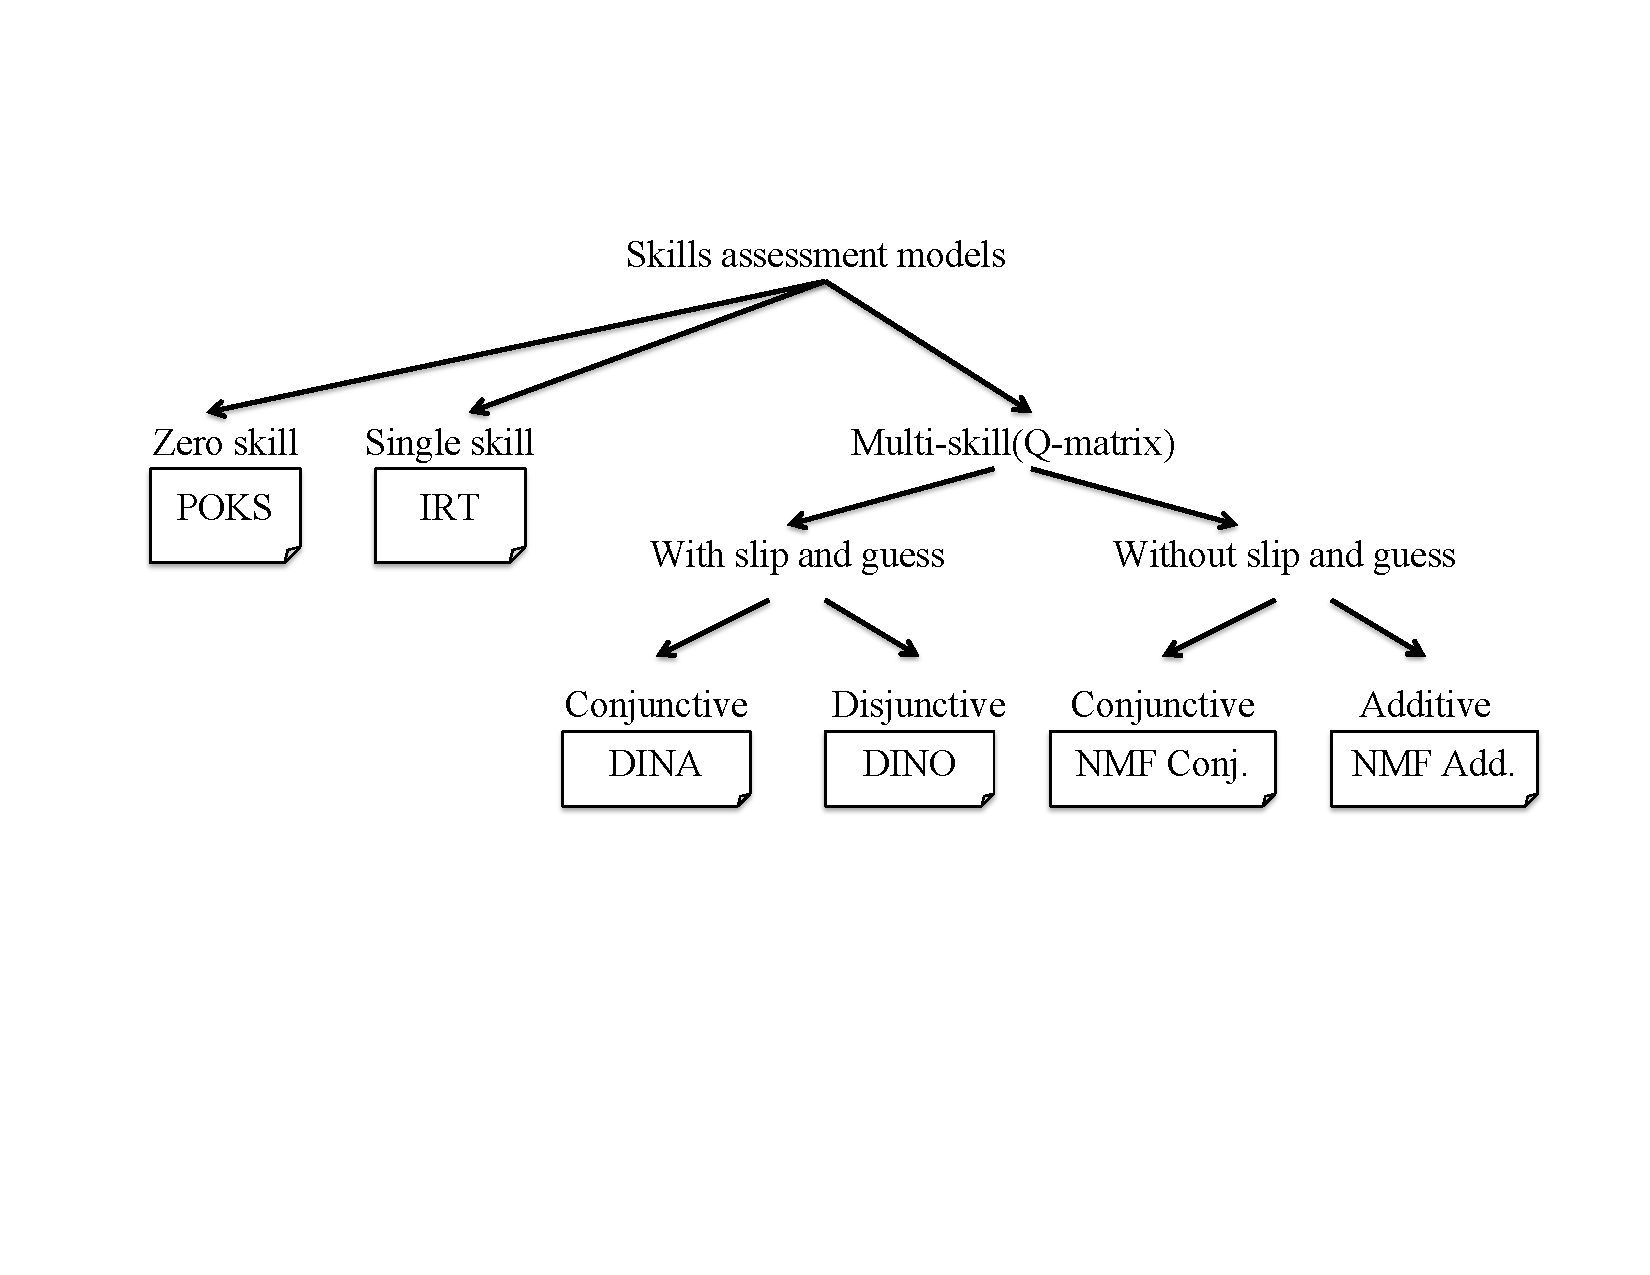
\includegraphics[trim=0.5cm 7cm 0.5cm 3cm,scale =0.5] {SkillsAssessments.pdf}
\caption{Skills assessment methods}
\label{AssessMethods}
\end{figure}

Considering  these techniques from the perspective of variety of skills in test outcome prediction, we can put them in the following categories: 

\begin{itemize}

\item Zero skill technique that predict item outcome based on observed items. POKS is the technique that is used as a zero skill student model.
\item Single skill approaches, where every item is linked to the same single skill. Item Response Theory (IRT) is the typical representative of this approach, but we also use the ``expected value'' approach which, akin to IRT, incorporates estimates of a the student's general skill and the item difficulty to yield a predicted item outcome.
\item Multi-Skills techniques that rely on Q-matrices to predict test outcome.  Deterministic Input Noisy And/Or (DINA/DINO), NMF Conjunctive and \ac{NMF} additive are the techniques we use in this study.

\end{itemize}  
Note that the ``expected value'' approach is considered as a baseline for our evaluations. 

The details of the different approaches are described below.

\section{Zero skill techniques}

\textit{Zero skill techniques} are so called because they make no explicit reference to latent skills.  They are based on the Knowledge Space theory of Doignon and Falmagne \citep{Doignon1999,desmarais:umuai:2006}, which does not directly attempt to model underlying skills but instead rely on observable items only.  An individual's knowledge state is represented as a subset of these items. In place of representing skills mastery directly, they leave the skills assessment to be based on the set of observed and predicted item outcomes which can be done in a subsequent phase. 

POKS is one of the models adopted in our study that is a derivative of Knowlege Space Theory.  POKS stands for Partial Order Knowledge Structures.  It is a more constrained version of Knowledge Spaces theory \citep{desmarais:umuai:1995}.  POKS assumes that items are learned in a strict partial order.  It uses this order to infer that the success to hard items increases the probability of success to easier ones, or conversely, that the failure to easy items decreases the chances of success to harder ones.

\subsection{Knowledge Spaces and Partial Order Knowledge Structures (POKS)}

Items are generally learnt in a given order. Children learn easy problems first, then harder problems. It reflects the order of learning a set of items in the same problem domain. POKS learns the order structure from test data in a probabilistic framework. For example in figure \ref{fig2} four items are shown in a partial order of knowledge structure. It is required for an examinee to be able to answer $i_{4}$ in order to solve $i_{3}$ and $i_{2}$. Also for solving $i_{1}$, one should be able to answer $i_{2}$, $i_{3}$ and $i_{4}$. if an examinee was not able to answer $i_{4}$ then he would have less chance to answer correctly other items.

\begin{figure}
\begin{footnotesize} \begin{diagram}[notextflow]    & & i_{1}:\frac{4}{\frac{12}{3}}+\frac{3}{5}=\frac{8}{5} & &   \\    & \ldTo_a & & \rdTo_b &   \\    & & & &   \\   i_{2}:\frac{4}{\frac{12}{3}}=\frac{4{\times}3}{12}=\frac{12}{12}=1 & & & & i_{3}:1+\frac{3}{5}=\frac{8}{5}  \\    & & & &   \\    & \rdTo_c & & \ldTo_d &   \\    & & i_{4}:2{\times}\frac{1}{2}=1 & &    \\  \end{diagram} \end{footnotesize}

\caption{Partial Order Structure of 4 items}

\label{fig2} 
\end{figure}

This is reflected in the results matrix $\mathbf{R}$ by closure constraints on the possible knowledge states. Defining a student knowledge state as a subset of all items (i.e. a column vector in $\mathbf{R}$), then the space of valid knowledge states is closed under union and intersection according to the theory of Knowledge spaces \citep{Doignon1985}. In our study, we will relax this constraint to a closure under union, meaning that the union of any two individual knowledge states is also a valid knowledge state. This means that the constraints can be expressed as a partial order of implications among items \citep{desmarais:umuai:1996}, termed a Partial Order Knowledge Structure (POKS). The algorithm to derive such structures from the data in $\mathbf{R}$ relies on statistical tests \citep{desmarais:umuai:1996,desmarais:2005}.

A knowledge structure can be represented by an Oriented incidence matrix, O, or by an Adjacency matrix, A. In the oriented incidence matrix, rows are edges and columns are nodes of the graph. The value of -1 shows the start node of an edge and 1 indicates the end of an edge. Therefore for each row (edge) there is only one pair of (-1,1) and the rest of cells are 0. In adjacency matrix both rows and columns are Items and if there is a link between a pair of items (for example $i\rightarrow j$) there should be a 1 in $A_{ij}$ otherwise it is 0. Figure \ref{fig3IMAM} shows the corresponded oriented incidence matrix and adjacency matrix of the structure in figure~\ref{fig2}. 


\begin{figure}
\[
\begin{array}{ccccc}
\begin{array}{cc}
 & \begin{array}{cccc}
i_{1} & i_{2} & i_{3} & i_{4}\end{array}\\
\begin{array}{c}
a\\
b\\
c\\
d
\end{array} & \left(\begin{array}{cccc}
-1 & 1 & 0 & 0\\
-1 & 0 & 1 & 0\\
0 & -1 & 0 & 1\\
0 & 0 & -1 & 1
\end{array}\right)
\end{array} &  &  &  & \begin{array}{cc}
 & \begin{array}{cccc}
i_{1} & i_{2} & i_{3} & i_{4}\end{array}\\
\begin{array}{c}
i_{1}\\
i_{2}\\
i_{3}\\
i_{4}
\end{array} & \left(\begin{array}{cccc}
0 & 1 & 1 & 0\\
0 & 0 & 0 & 1\\
0 & 0 & 0 & 1\\
0 & 0 & 0 & 0
\end{array}\right)
\end{array}\\
\\
\\
O &  &  &  & A
\end{array}
\]


\caption{Oriented incidence matrix and Adjacency matrix}
\label{fig3IMAM}
\end{figure}


The structure of the partial order of items is obtained from a statistical hypothesis test that reckons the existence of a link between two items, say $A \rightarrow B$, on the basis of two Binomial statistical tests $P(B|A) > \alpha_1$ and $P(\neg A|\neg B) > \alpha_1$ and under a predetermined alpha error of an interaction test ($\alpha_2$).  The $\chi^2$ test is often used, or the Fisher exact test.  The values of $\alpha_1 = .85$ and $\alpha_2 = .10$ are chosen in this study across all experiments.

A student knowledge state is represented as a vector of probabilities, one per item.  Probabilities are updated under a Naive Bayes assumption as simple posterior probabilities given observed items.

Inference in the POKS framework to calculate the node's probability relies on standard Bayesian posteriors under the local independence assumption. The probability update for node $H$ given $E_1$,... $E_n$ can be written in following posterior odds form :
\begin{equation}
O(H|E_1,E_2, ... , E_n) = O(H) \prod_{i}^{n} \frac{P(E_i|H)}{P(E_i | \overline{H})}
\label{EQPOKSratio}
\end{equation}
where odds definition is $O(H|E) = \frac{P(H|E)}{1-P(H|E)}$. If evidence $E_i$ is negative for observation $i$, then the ratio $\frac{P(\overline{E_i}|H)}{P(\overline{E_i}|\overline{H})}$ is used.

\section{Single skill approaches}

Other approaches incorporate a single latent skill in the model. This is obviously a strong simplification of the reality of skilled performance, but in practice it is a valid approximation as results show. When a model uses single latent skill, in fact it projects all the skills mastery level in a form of unidimentional representation that implicitly combines all skills. Then there would be a single continuous skill variable which is a weighted average of the skills mastery levels of an examinee. 

In this section two approaches for modeling static test data are presented: The well established Item Response Theory (IRT) which models the relationship between observation and skill variable based on a logistic regression framework. It dates back to the 1960's and is still one of the prevailing approaches \citep{bakerKim2004}.  The second approach is a trivial approach we call Expected Prediction. This approach is used as a baseline in our experiments.

\subsection{IRT} 

The \textbf{IRT family} is based on a logistic regression framework. It models a single latent skill (although variants exists for modeling multiple skills) \cite{bakerKim2004}.  Each item has a difficulty and a discrimination parameter.

IRT assumes the probability of success to an item~$X_j$ is a function of a single ability factor~$\theta$: 
\[P(X_j\!=\!1\;|\;\theta) = \frac{1}{1+e^{-a_j(\theta-b_j)}}\]
In the two parameter form above, referred to as IRT-2pl, where parameters are:

\begin{itemize}
\item[$a$] represents the item discrimination;
\item [$b$] represents the item difficulty, and
\item [$\theta_i$] the ability of a single student.
\end{itemize}

Student, $\theta_i$, is estimated by maximizing the likelihood of the observed response outcomes probabilities:
\[ P(X_1, X_2, ..., X_j, \theta_i) = \prod_j P(X_j|\theta_i) \]
This corresponds to the usual logistic regression procedure.

The specific IRT skills assessment version is the Rash model, for which the discrimination parameter~$a$ is fixed to~$1$.  Fixing this parameter reduces over fitting, as the discrimination can sometimes take unrealistically large values. Note however that we do use the more general IRT-2pl model, which includes both~$a$ and $b$, for the synthetic data generation process and test outcome prediction in order to make this data more realistic (next chapters discuss data generation in details).

\subsection{Baseline Expected Prediction}

As a baseline model, we use the expected value of success to an item~$i$ by student~$j$, as defined by a product of odds:
\[ O(X_{ij}) =  O(X_i) O(S_j) \]
where $O(X_i)$ are the odds of success to item~$i$ and $O(S_j)$ are the odds of success of student~$j$.  Both odds can be estimated from a sample.  Recall that the transformation of odds to probability is $P(X) = 1/(1+O(X))$, and conversely $O(X) = P(X)/(1 - P(X))$. Probabilities are estimated using the Laplace correction: $P(X) = (f(x\!=\!1) + 1) / (f(x\!=\!1) + f(x\!=\!0) + 2)$


\section{Multi-skills techniques}

Finally the last category of student skills assessment models are considering student test result with multiple latent skills. Representation of multiple skills is possible in the form of a Q-matrix where skills are mapped to each item. As explained before there exists different types of Q-matrices that each type represent a unique interpretation. The following sections will describe different skills assessment models along with their specific type of Q-matrix.


Still there exists two types of methods in this category: 
\begin{itemize}
\item Models that infer a Q-matrix from test result data such as models that uses matrix factorization techniques.
\item Models that require a predefined Q-matrix to predict test outcome. These techniques can not directly infer the Q-matrix but they can refine an existing expert defined Q-matrix.
\end{itemize}

Deriving a Q-matrix from a test result matrix was always challenging. Some models require a pre-defined Q-matrix. In some cases an expert defined Q-matrix is available but minor mistakes in mapping skills to items are always possible even by an expert. The basic challenge is to derive a perfect Q-matrix out of a test result matrix to give it as an input parameter to some models. This challenge also creates other challenges  such as optimum number of latent skills for a set of items in a test outcome. Sometimes there exists more that single Q-matrix associated with a test result with different number of skills. Finding the optimum number of skills to derive a Q-matrix is a question that is given in more details in section \ref{EDM2012}. 

Given the number of latent skills, there exists few techniques to derive a Q-matrix for models that require one. Cen et al. \citep{Cen2005,Cen2006} have used Learning FactorAnalysis technique(LFA) technique to improve the initially hand built Q-matrix which maps fine-grained skills to questions. They used log data which is based on the fact that the knowledge state of student dynamically changes over time as the student learns. In the case of static data of student knowledge, Barnes \citep{Barnes06} developed a method for this mapping which works based on a measure of the fit of a potential Q-matrix to the data. It was shown to be successful as well as Principle Component Analysis for skill clustering analysis. In our experiment we use NMF as a technique to derive a Q-matrix given an optimum number of latent skills. Later in this section we will introduce NMF in more details. Section \ref{ITS2012} describes how to derive a conjunctive model of Q-matrix from a student test result.

For real datasets there exists few expert defined Q-matrices. To use them as an input parameter of student skills assessment models we need to refine them. Section \ref{edm2014} gives few approaches to this problem.


\subsection{Types of Q-matrix (examples) }

There are three models for the Q-matrix which are useful based on the context of the problem domain. The most important one is the conjunctive model of the Q-matrix which is the standard interpretation of the Q-matrix. In figure \ref{fig1} an example of conjunctive model of Q-matrix is shown. Examinee $e_{1}$ answered item $i_{1}$ and item $i_{4}$ because he has mastered in the required skills but although he has skill $s_{1}$ he couldn't answer item $i_{3}$ which requires skill $s_{2}$ as well.

\begin{figure}
\begin{footnotesize} 
\[
\begin{array}{ccc}
\begin{array}{cc}
 & \textrm{Examinee}\\
 & \begin{array}{cccc}
e_{1} & e_{2} & e_{3} & e_{4}\end{array}\\
\mathrm{\begin{sideways}Items\end{sideways}}\begin{array}{c}
i_{1}\\
i_{2}\\
i_{3}\\
i_{4}
\end{array} & \left[\begin{array}{cccc}
1 & 0 & 1 & 0\\
0 & 1 & 0 & 0\\
0 & 0 & 1 & 0\\
1 & 0 & 0 & 0
\end{array}\right]
\end{array} & \begin{array}{cc}
 & \textrm{Skills}\\
 & \begin{array}{ccc}
s_{1} & s_{2} & s_{3}\end{array}\\
\mathrm{\begin{sideways}Items\end{sideways}}\begin{array}{c}
i_{1}\\
i_{2}\\
i_{3}\\
i_{4}
\end{array} & \left[\begin{array}{ccc}
1 & 0 & 0\\
0 & 1 & 1\\
1 & 1 & 0\\
1 & 0 & 1
\end{array}\right]
\end{array} & \begin{array}{cc}
 & \textrm{Examinees}\\
 & \begin{array}{cccc}
e_{1} & e_{2} & e_{3} & e_{4}\end{array}\\
\mathrm{\begin{sideways}Skills\end{sideways}}\begin{array}{c}
s_{1}\\
s_{2}\\
s_{3}
\end{array} & \left[\begin{array}{cccc}
1 & 0 & 1 & 0\\
0 & 1 & 1 & 1\\
1 & 1 & 0 & 0
\end{array}\right]
\end{array}\\
\\
R & Q & S
\end{array}
\]
 \end{footnotesize} \caption{An example for Conjunctive model of Q-matrix}


\label{fig1} 
\end{figure}

%, but for expert-defined Q-matrices in our study we consider similar weights for each skills of an item\note{they will not be equal when the Q-matrix is from a factorization}\note{You are right, I was thinking about the data generation phase, in data generation process for random Q-matrix generation we consider same weights 
The other type is the additive model of Q-matrix. Compensatory or additive model of skills is an interpretation of a Q-matrix where skills have weights to yield a success for that item. For example, considering an item requires two skills $a$ and $b$ with the same weight each. Then each skill will contribute equally to yield a success of the item. In the compensatory model of Q-matrix, each skills increase the chance of success based on its weight. It is possible to have different weights for skills where skills for each item will sum up to~$1$. Figure \ref{fig1Add} represents an example of an additive model of Q-matrix with its corresponding result matrix. The value $R_{ij}$  can be considered as a probability that examinee $i$ can succeed item $j$.

\begin{figure}
\begin{footnotesize} 
\[
\begin{array}{ccc}
\begin{array}{cc}
 & \textrm{Examinee}\\
 & \begin{array}{ccccccc}
e_{1} && e_{2} && e_{3} && e_{4}\end{array}\\
\mathrm{\begin{sideways}Items\end{sideways}}\begin{array}{c}
i_{1}\\
i_{2}\\
i_{3}\\
i_{4}
\end{array} & \left[\begin{array}{cccc}
1 & 0 & 1 & 0\\
0.5 & 1 & 0.5 & 0.5\\
0.5 & 0.5 & 1 & 0.5\\
0.66 & 0.66 & 0.66 & 0.33
\end{array}\right]
=
\end{array} & \begin{array}{cc}
 & \textrm{Skills}\\
 & \begin{array}{ccccc}
s_{1} & &s_{2} && s_{3}\end{array}\\
\mathrm{\begin{sideways}Items\end{sideways}}\begin{array}{c}
i_{1}\\
i_{2}\\
i_{3}\\
i_{4}
\end{array} & \left[\begin{array}{ccc}
1 & 0 & 0\\
0 & 0.5 & 0.5\\
0.5 & 0.5 & 0\\
0.33 & 0.33 & 0.33
\end{array}\right]
\end{array} & \begin{array}{cc}
 & \textrm{Examinees}\\
 & \begin{array}{cccc}
e_{1} & e_{2} & e_{3} & e_{4}\end{array}\\
\mathrm{\begin{sideways}Skills\end{sideways}}\begin{array}{c}
s_{1}\\
s_{2}\\
s_{3}
\end{array} & \left[\begin{array}{cccc}
1 & 0 & 1 & 0\\
0 & 1 & 1 & 1\\
1 & 1 & 0 & 0
\end{array}\right]
\end{array}\\
\\
R & Q & S
\end{array}
\]
 \end{footnotesize} \caption{An example for Additive model of Q-matrix}


\label{fig1Add} 
\end{figure}

Finally, in the disjunctive model of Q-matrix, there is a disjunction between skills of an item to achieve a success. At least one of the required skills should be mastered in order to succeed that item. Figure \ref{fig1Dis} shows an example of this type. For example examinee $e_{3}$ has both skills $S_{1}$ and $S_{2}$ and all items require either $S_{1}$ or $S_{2}$; then he should be able to answer all items in the test outcome. 



\begin{figure}
\begin{footnotesize} 
\[
\begin{array}{ccc}
\begin{array}{cc}
 & \textrm{Examinee}\\
 & \begin{array}{cccc}
e_{1} & e_{2} & e_{3} & e_{4}\end{array}\\
\mathrm{\begin{sideways}Items\end{sideways}}\begin{array}{c}
i_{1}\\
i_{2}\\
i_{3}\\
i_{4}
\end{array} & \left[\begin{array}{cccc}
1 & 0 & 1 & 0\\
1 & 1 & 1 & 1\\
0 & 1 & 1 & 1\\
1 & 1 & 1 & 0
\end{array}\right]
\end{array} & \begin{array}{cc}
 & \textrm{Skills}\\
 & \begin{array}{ccc}
s_{1} & s_{2} & s_{3}\end{array}\\
\mathrm{\begin{sideways}Items\end{sideways}}\begin{array}{c}
i_{1}\\
i_{2}\\
i_{3}\\
i_{4}
\end{array} & \left[\begin{array}{ccc}
1 & 0 & 0\\
0 & 1 & 1\\
0 & 1 & 0\\
1 & 0 & 1
\end{array}\right]
\end{array} & \begin{array}{cc}
 & \textrm{Examinees}\\
 & \begin{array}{cccc}
e_{1} & e_{2} & e_{3} & e_{4}\end{array}\\
\mathrm{\begin{sideways}Skills\end{sideways}}\begin{array}{c}
s_{1}\\
s_{2}\\
s_{3}
\end{array} & \left[\begin{array}{cccc}
1 & 0 & 1 & 0\\
0 & 1 & 1 & 1\\
1 & 1 & 0 & 0
\end{array}\right]
\end{array}\\
\\
R & Q & S
\end{array}
\]
 \end{footnotesize} \caption{An example for Disjunctive model of Q-matrix}


\label{fig1Dis} 
\end{figure}

Comparing these three types together, in the same condition for student skills mastery level we can find out that the average success rate in the test result data is the highest for disjunctive type and the lowest for conjunctive type. Also if we consider the Q-matrix as a single skill per item, then the definition of conjunctive, disjunctive and additive model of Q-matrix does not affect the final result.


\subsection{Non-Negative Matrix Factorization (\ac{NMF})}
\label{NMF_MODEL_ASSESS}

Different techniques and methods in the field of data mining were used to derive a Q-matrix. Matrix factorization is one of the most important one in this area. Matrix factorization is a method to decompose a matrix into two or more matrices. Singular Value Decomposition (SVD) and NMF are well known examples of such methods. Beyond skill modelling, it is an important technique in different fields such as bioinformatics, and vision, to name but a few. It has achieved great results in each of these fields. For skills assessment, using tensor factorization, a generalization of matrix factorization to a hypercube instead of matrix and where one dimension represents the time, Thai-Nghe et al. \citep{Nguyen2011} have shown that the approach can lead to assessments that reach prediction accuracies comparable and even better than well established techniques such as Bayesian Knowledge Tracing \citep{corbett:umuai:1995}. Matrix factorization can also lead to better means for mapping which skills can explain the success to specific items. In this research, we use NMF as a skill assessment method that infers a Q-matrix with multiple skills.

Assume $\mathbf{R}$ is a result matrix containing student test results of ${n}$ items (questions or tests) and ${m}$ students. \ac{NMF} decompose the non-negative $\mathbf{R}$, as the product of two non-negative matrices as shown in equation\protect\eqref{eq:1}:
\begin{equation}
\mathbf{R}\approx\mathbf{Q}\mathbf{S}\label{eq:1}
\end{equation}
where $\mathbf{Q}$ and $\mathbf{S}$ are ${n}\times{k}$ and ${k}\times{m}$ respectively. $\mathbf{Q}$ represents a Q-matrix which maps items to skills and $\mathbf{S}$ represents the skill mastery matrix that represents the mastered skills for each student. ${k}$ is called as the rank of factorization which is the same as number of latent skills. Equation \ref{eq:1} represents an additive type of Q-matrix.

For example in the following equation, assume that we know the skills behind each item which means we know the exact Q-matrix and also we know the skills mastery matrix as well. In this example the product of $\mathbf{Q}$ and $\mathbf{S}$ will reproduces the result matrix. Given a result matrix, we want to decompose this result matrix into the expected Q-matrix and skill mastery matrices. Since the Q-matrix is a single skill per item then the type of Q-matrix does not affect the inference of the result matrix.

\[
\begin{array}{ccccc}
\begin{array}{cc}
 & \textrm{Examinee}\\
\mathrm{\begin{sideways}Items\end{sideways}} & \left[\begin{array}{cccc}
1 & 0 & 1 & 0\\
1 & 1 & 0 & 0\\
1 & 0 & 1 & 0\\
0 & 1 & 0 & 1
\end{array}\right]
\end{array} & = & \begin{array}{cc}
 & \textrm{Skills}\\
\mathrm{\begin{sideways}Items\end{sideways}} & \left[\begin{array}{ccc}
1 & 0 & 0\\
0 & 0 & 1\\
1 & 0 & 0\\
0 & 1 & 0
\end{array}\right]
\end{array} & \times & \begin{array}{cc}
 & \textrm{Examinees}\\
\mathrm{\begin{sideways}Skills\end{sideways}} & \left[\begin{array}{cccc}
1 & 0 & 1 & 0\\
0 & 1 & 0 & 1\\
1 & 1 & 0 & 0
\end{array}\right]
\end{array}\\
\\
R &  & Q &  & S
\end{array}
\]

The prominent characteristic of \ac{NMF} is the non-negative constraint on the decomposed elements. \ac{NMF} imposes this constraint and consequently all those values in the decomposed elements are non-negative. The clear point of this decomposition is that there can be different solutions. Although the constraint of non-negative elements eliminate some solutions, there remain many different solutions for this factorization.

Considering the large space of solutions to $\mathbf{R}\approx\mathbf{Q}\mathbf{S}$, it implies different algorithms may lead to different solutions. Many algorithms for matrix factorization search the space of solutions to equation \eqref{eq:1} by gradient descent. These algorithms can be interpreted as rescaled gradient descent, where the rescaling factor is optimally chosen to ensure convergence. Most of factorization algorithms operate iteratively in order to find the optimal factors. At each iteration of these algorithms, the new value of $\mathbf{Q}$ or $\mathbf{S}$ (for \ac{NMF}) is found by multiplying the current value by some factor that depends on the quality of the approximation in Eq. \eqref{eq:1}. It was proved that repeated iteration of the update rules is guaranteed to converge to a locally optimal factorization~\citep{seung2001algorithms}. We refer the reader to \citep{Berry2007} for a more thorough and recent review of this technique which has gained strong adoption in many different fields. 

Gradient decent is one of the best known approaches for implementing  \ac{NMF}.  If $k$ is less than the minimum of $m$ and $n$, finding the exact $\mathbf{Q}$ and $\mathbf{S}$ matrices which satisfy $\mathbf{R}=\mathbf{Q}\mathbf{S}$, can entail a loss of information. Therefore this algorithm tries to get the best estimation for $\mathbf{Q}$ and $\mathbf{S}$ to make $\mathbf{R}\approx\mathbf{Q}\mathbf{S}$ more accurate. Based on the definition of gradient descent method, a cost function should be defined to quantify the quality of the approximation. This cost function can be a measure of distance between two non-negative matrices $\mathbf{R}$ and $\mathbf{Q}\mathbf{S}$. It  can be the Euclidean distance between these two matrices as shown in equation \eqref{eq:3} where $\mathbf{Q}_{i}$ is a row vector of $\mathbf{Q}$ and $\mathbf{S}_{j}$ is a column vector of $\mathbf{S}$ and $\mathbf{R}_{ij}$ is cell $(i,j)$ of $\mathbf{R}$.

\begin{equation}
\left\Vert \mathbf{R}-\mathbf{Q}\mathbf{S}\right\Vert ^{2}=\sum_{{\scriptscriptstyle ij}}(\mathbf{R}_{ij}-\mathbf{Q}_{i}\mathbf{S}_{j})^2\label{eq:3}
\end{equation}


  
Another cost function  is based on the Kullback-Leibler divergence, which measures the divergence between $\mathbf{R}$ and $\mathbf{Q}\mathbf{S}$ as shown in equation \eqref{eq:4}. 
\begin{equation}
D(\mathbf{R}||\mathbf{Q}\mathbf{S})=\sum_{{\scriptscriptstyle ij}}(\mathbf{R}_{ij}log\frac{\mathbf{R}_{ij}}{\mathbf{Q}_{i}\mathbf{S}_{j}}-\mathbf{R}_{ij}+\mathbf{Q}_{i}\mathbf{S}_{j})\label{eq:4}
\end{equation}

In both approaches, the goal is to minimize the cost function where they are lower bounded by zero and it happens only if $\mathbf{R}=\mathbf{Q}\mathbf{S}$ \citep{seung2001algorithms}. For simplicity we just consider the cost function based on the Euclidean distance.

The gradient descent algorithm used to minimize the error is iterative and in each iteration we expect a new estimation of the factorization. We will refer to the estimated Q-matrix{ as} $\hat{\mathbf{Q}}$ and{ the} estimated Skill mastery matrix{ as} $\hat{\mathbf{S}}$.  The iterative gradient descent algorithm should change $\mathbf{Q}$ and $\mathbf{S}$ to minimize the cost function. This change should be done by an update rule. Lee and Seung \citep{seung2001algorithms} found the following update rule in equation \eqref{eq:5}. These update rules in equation \eqref{eq:5} guarantee that the Euclidean distance $\left\Vert \mathbf{R}-\mathbf{Q}\mathbf{S}\right\Vert $ is non increasing during the iteration of the algorithm.

\begin{equation}
\begin{aligned}\hat{\mathbf{S}}\leftarrow\hat{\mathbf{S}}\frac{(\mathbf{\hat{Q}}^{T}\mathbf{R})}{(\hat{\mathbf{Q}}^{T}\mathbf{\hat{Q}}\hat{\mathbf{S}})}\end{aligned}
\hspace{20mm}\begin{aligned} & \mathbf{\hat{Q}}\leftarrow\mathbf{\hat{Q}}\frac{(\mathbf{R}\mathbf{\hat{\mathbf{S}}}^{T})}{(\mathbf{\hat{Q}}\mathbf{\hat{\mathbf{S}}}\mathbf{\hat{\mathbf{S}}}^{T})}\end{aligned}
\label{eq:5}
\end{equation}


The initial value for Q and S are usually random but they can be adjusted to a specific method of \ac{NMF} library to find the best seeding point.



Barnes \citep{Barnes2005} proposed equation \ref{eq:6} for conjunctive model of Q-matrix where the operator $\neg$ is the boolean negation that maps 0 values to 1 and other values to 0. In this way, if an examinee that mastered all required skills for an item, he will get 1 in the result matrix otherwise he will get a 0 value, even if the required skills are partially mastered.

In fact if we apply a boolean negation function to both sides of the equation \ref{eq:6}, we will see that the $\neg\mathbf{R}$ matrix is a product of two matrices, $\mathbf{Q}$ and $\neg\mathbf{S}$

\begin{equation}
\mathbf{R}=\neg\left(\mathbf{Q}\left(\neg\mathbf{S}\right)\right)\label{eq:6}
\end{equation}

In next sections of this chapter the application of NMF on conjunctive type of Q-matrix and how this technique can derive a Q-matrix from a test result is given in details.

Besides its use for student skills assessment and for deriving a Q-matrix, matrix factorization is also a widely used technique in recommender systems. See for eg. \citet{koren2009matrix}  for a brief description of some of the adaptation of these techniques in recommender systems. 



%\subsection{Recommender systems and matrix factorization}

%In the field of recommender systems, linear models have taken a central role.  Models based on matrix factorization fared particularly well in recent years.  They allow the alignment of users and votes along a few common latent factors, which was proven very efficient for predicting votes.  A culminant demonstration of the efficiency of these techniques was given in the Netflix contest~\cite{journals/sigkdd/BellK07,conf/kdd/JahrerTL10}.

%The recommender systems techniques were recently applied in the field of student skills modeling~\cite{conf/its/CetintasSXH10,Toscher2010,Nguyen2011}.  The 2010 KDD Cup was held over educational data and surely helped in bringing attention of the recommender community over the task of student skills assessment.  A comparison with the widely recognized Bayesian Knowledge Tracing approach showed that it compared favorably~\cite{Nguyen2011}. Nguyen et al.\ used a multi-relational matrix and tensor-based factorization to model latent factors (skills) and the time effect to predict student success~\cite{Nguyen2011,conf/csedu/Thai-NgheDHNS11}.

%The above work was conducted over dynamic student performance data.  It consists of logs of success and failures of students on exercises as they interact with a learning system environment.  These environments typically exercise the same skills over multiple problem, and often provide hints to help solve the exercises as the student faces difficulties. Obviously, learning will occur during the interaction. In fact, the same question item can be presented many times, failed one or mores time and succeeded in the end.  This is in contrast to test data where the items are presented at once without any opportunity to access learning material.  We refer to this data as static performance data.

%\note{birnbaum:1968 and the connection of IRT and recoomender systems and MF??}
%A large body of methods have been developed for assessing student skills with static performance data (see~\cite{Desmarais2011} for a review).  For the vast majority, these methods are either non linear models or general linear models (for eg.~logistic regression). The most widely used one is Item Response Theory (IRT)~\cite{birnbaum:1968}.  Although it and it dates back to almost 50~years, it remains one of the most prominant and an active field of research in psychometrics (for eg.~\cite{bakerKim2004}).

%\subsection{Similarity with recommender systems and assumptions}

%Equation~(\ref{eq:nmf}) is analoguous to the decomposition of the (\textit{item} $\times$ \textit{user}) votes matrix into two smaller matrices: the (\textit{item} $\times$ \textit{preference}) and (\textit{preference} $\times$ \textit{user}) matrices.  However, the the votes matrix is typically sparse and different means have been developed to accomodate matrix factorization techniques with sparse matrices, and to compensate for predictions based on highly uneven number of votes in columns and rows that tend to negatively affect the predictive performance of algorithms.


\subsection{Deterministic Input Noisy And/Or (DIAN/DINO)}

The other skills assessment models we consider are based on what is referred to as Deterministic Input Noisy And/Or (DINO/DINA) \cite{junker2001cognitive}.  They also rely on a Q-matrix and they can not in themselves infer a Q-matrix from a test result matrix, and instead require a predefined Q-matrix for the predictive analysis. The DINA model (Deterministic Input Noisy And) corresponds to the conjunctive model whereas the DINO (Deterministic Input Noisy Or) corresponds to the disjunctive one, where the mastery of a single skill is sufficient to succeed an item.  The acronyms makes reference to the AND/OR gates terminology.

These models predict item outcome based on three parameters: the slip and guess factors of items, and the different ``gate'' function between the student's ability and the required skills.  The gate functions are equivalent to the conjunctive and disjunctive vector product logic described for the matrix factorization above.  In the DINA case, if all required skills are mastered, the result is~1, and 0~otherwise. Slip and guess parameters are values that generally vary on a~$[0,0.2]$ scale. In the DINO case, mastery of any skills is sufficient to output~1.  Assuming~$\xi$ is the output of the corresponding DINA or DINO model and~$s_j$ and~$g_j$ are the slip and guess factors, the probability of a successful outcome to item~$X_{ij}$ is:
\begin{equation}
 P(X_{ij} \!=\! 1 \; | \; \xi_{ij}) \,=\, (1-s_j)^{\xi_{ij}} g_j^{1-\xi_{ij}}
\label{DinoEQ}
\end{equation}

The DINO model is analog to the DINA model, except that mastery follows the disjunctive framework and therefore~$\xi_{ij}=1$ if \textit{any} of the skills required by item~$j$ are mastered by student~$i$.

A few methods have been developed to estimate the slip and guess parameters from data and we use the one implemented in the R~CDM package \citep{Robitzsch2012}.

\subsection{Alternate Least-square Factorization (ALS)}
\label{ALS-Def}



The {Alternate Least-Square Factorization (ALS)} method is defined in \cite{Desmarais2013aied} which is also a factorization method that can infer an initial Q-matrix to estimate its parameters, or refine a predefined Q-matrix given as a starting point. The next sections in this chapter introduce a methodology to refine a existing Q-matrix in more details.

%\note{it was written that it cannot do a factorization without a Q-matrix, but this is not correct.  Just as NMF, it requires a starting point, but it can be a random starting point.}\note{ Behzad Says: Does it give you a correct guess for any random seeding point? as far as I remember, different random points gave back different Q-matrices, if it's true then it's not a reliable technique to derive a Q-matrix}

Starting with the results matrix ~$\mathbf{R}$ and an initial Q-matrix, $\mathbf{Q}_0$, a least-squares estimate of the skills matrix ~$\mathbf{\hat{S}}_0$ can be obtained by:

\begin{equation}
    \mathbf{\hat{S}}_0 = (\mathbf{Q}_0^{\mathrm{T}}  \, \mathbf{Q}_0)^{-1} \, \mathbf{Q}_0^{\mathrm{T}} \, \mathbf{R} \label{eq:shat1}
\end{equation}


The initial matrix~$\mathbf{{Q}}_0$ is the expert defined Q-matrix. Then, a new estimate of the Q-matrix, $\mathbf{\hat{Q}}_1$, is again obtained by the least-squares estimate:
\begin{equation}
  \mathbf{\hat{Q}}_1 = \mathbf{R} \, \mathbf{\hat{S}}_0^{\mathrm{T}} \, (\mathbf{\hat{S}}_0 \, \mathbf{\hat{S}}_0^{\mathrm{T}})^{-1} \label{eq:qhat2}
\end{equation}

And so on for estimating~$\mathbf{\hat{S}}_1$, ~$\mathbf{\hat{Q}}_2$, ... Alternating between equations~(\ref{eq:shat1}) and~(\ref{eq:qhat2}) yields progressive refinements of the matrices~$\mathbf{\hat{Q}}_i$ and ~$\mathbf{\hat{S}}_i$ that more closely approximate~$\mathbf{R}$ in equation~(\ref{eq:nmf}).  The convergence is based on a predefined delta between iterations. In our experiments we consider delta as $0.001$ that makes the algorithm to converge after few iterations. This performance makes the technique many times more efficient than factorizations that rely on gradient descent, for example.

The ALS factorization is \textit{compensatory} in the above description.  A \textit{conjunctive} version can be obtained by inverting the values of the $\mathbf{R}$~matrix~\citep{Desmarais2012b}.  

It is worth mentioning that, by starting with non negative matrices ~$\mathbf{{Q}}_0$ and ~$\mathbf{R}$, the convergence process will generally end with positive values for both matrices ~$\mathbf{\hat{Q}}_i$ and ~$\mathbf{\hat{S}}_i$. The vast majority of values obtained are between 0.5 and 1.5 if both the results matrix and the initial Q-matrix have {0,1} values. Also regularization terms could be used in the implementation of the algorithm to force non-negative or integer values.

Note that ~$(\mathbf{Q}_0^{\mathrm{T}} \, \mathbf{Q}_0)$ or ~$(\mathbf{\hat{S}}_0 \,\mathbf{\hat{S}}_0^{\mathrm{T}})_0$ may not be invertable, for example in the case where the matrix~$\mathbf{Q}_0$ is not column full-rank, or the matrix~$\mathbf{S}_0$ is not row full-rank.  This is resolved by adding a very small Gaussian noise before attempting the inverse.  Ensuring the choice of a relatively insignificant noise does not affect the end result for our purpose. 


\section{Recent improvements}

Let us get back to the main contribution of the thesis:  Assessing model fit on the basis of the goodness of fit measure with predictive performance analysis of real and synthetic data. The previous sections of this chapter introduced skills assessment techniques to obtain the predictive performance of a dataset. Some methods infer a Q-matrix and some other not even infer it but require a predefined one. Challenges are not limited to inferring a Q-matrix out of data: the number of latent skills is also unknown. For some real dataset there exists at least one pre-defined Q-matrix  by an expert which could have potential mistakes and requires to be refined. These are some challenges that should be addressed as a complementary steps to predictive performance analysis.

The rest of this chapter presents researches that are complementary steps of the main contribution of this thesis. The general perspective of section \ref{ITS2012} is to find a way for deriving the Q-matrix from data, along with a Skills mastery matrix. Section \ref{ITS2012} is inspired by \citet{desmarais2012mapping} that was published in ITS conference. This article aims to find a method to derive these matrices for different types of Q-matrices. This is a valuable and challenging task. Finding the number of latent skills (i.e. the common dimension between matrices $\mathbf{Q}$ and~$\mathbf{S}$) is another important task that is described in section \ref{ITS2012} . The text of section \ref{EDM2012} is mainly borrowed form \citet{Beheshti2012Numbers} work that was published on EDM conference. Finally, in section \ref{edm2014} few methods is introduced to validate tasks to skills mapping which is also applicable for the refinement of a Q-matrix. Parts of section \ref{edm2014} is taken from \citet{desmarais2014refinement} publication in EDM conference.


\section{NMF on single skill and multi-skill conjunctive Q-matrix}
\label{ITS2012}

A few studies have shown that a mapping of skills to items can, indeed, be derived from data \citep{winters2006,desmarais2011conditions}. \citet{Winters2006} showed that different data mining techniques can extract item topics, one of which is matrix factorization. He showed that NMF works very well for synthetic data, but the technique's performance with real data was degraded. The above studis show that only highly distinct topics such as mathematics and French can yield a perfect mapping. Biology and history were the other topics in this research which were named as general topics. Clustering of these topics was not accurate because they are factual knowledge and they are not comparable with some topics like mathematics.

These results were later corroborated by \citet{desmarais2011conditions} who also used simulated data to show that the low discrimination power of some topics might be explained by their lower weight in terms of skill factors, when compared to other factors such as item difficulty and student ability.

The factorization methods in the studies mentioned above rely on the standard matrix operators which was in formula \ref{eq:1} and therefore can be considered as compensatory models of Q-matrix which was explained in the previous chapter. Actually, these studies rely on single skill per item type of Q-matrix and there was not a combination of skills for any item, thus the simple model of factorization will work. 

To follow up the on previous studies \citep{Barnes2005,desmarais2011conditions,Winters07} There is still a chance to apply NMF technique to equation \ref{eq:6}. The goal of the contribution in \citet{desmarais2012mapping} paper is to determine if NMF can successfully derive a conjunctive model of Q-matrix, where skills do not add up to increase the chances of success to an item, but instead are necessary conditions.


\subsection{Simulated data}
%\note{This section and the following few after seem to be taken verbatim from the ITS2012.  First, this has to be EXPLICITELY NENTIONED.  Very important or otherwise it can be considered plagiarism.  It is ok to take verbatim some parts of existing papers in a thesis where you are co-author, but it has to be mentioned, especially if you are not fisrt author.  Second, it does not fit very well in this section.  It is written as a new experiment, whereas we are in the review of past work. }
To validate the technique, The methodology of this research relies on simulated data. Although it lacks the external validity of real data, it remains the most reliable means of obtaining test results data for which the underlying, latent skills structure is perfectly known. Therefore, assessing the technique over simulated data is a reasonable first step to establish the validity the approach under controlled conditions. 

Whilst the underlying model  is shown in previous sections, we describe an overall view of simulated data generation of this paper. More details on synthetic data generation is given in chapter \ref{sec:Syn}.

A first step to obtain data of simulated examinee test results is to define a Q-matrix composed of $j$ skills and $k$ items. They chose to define a Q-matrix that spans all possible combinations of 6 skills with a maximum of two skills per item, and at least one skill per item. A total of 21 items spans this space of combinations. This matrix is shown in Figure \ref{figqmatrixandResutM}. Items 1 to 15 are two-skills and items 16 to 21 are single-skill. 

\begin{figure}[ht]
\centering

\subfigure[Q-matrix of 6 skills and for which 21 items are spanning the full set of 1 and 2 skill combinations]{
   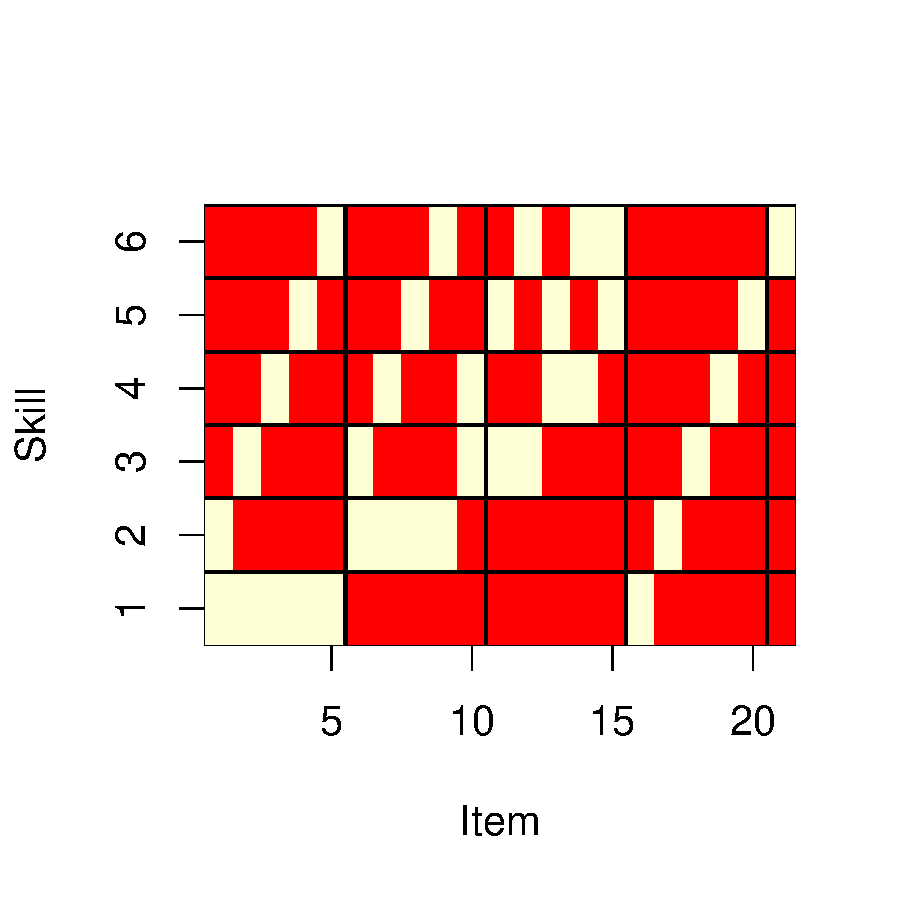
\includegraphics[scale =0.5] {ExpectedQ}\label{PerfectQ}
 }\quad
 \subfigure[Simulated data example of 100 examinees with parameters: slip: 0.1, guess: 0.2, skills difficulties: ($0.17$, $0.30$, $0.43$, $0.57$, $0.70$, $0.83$)]{
   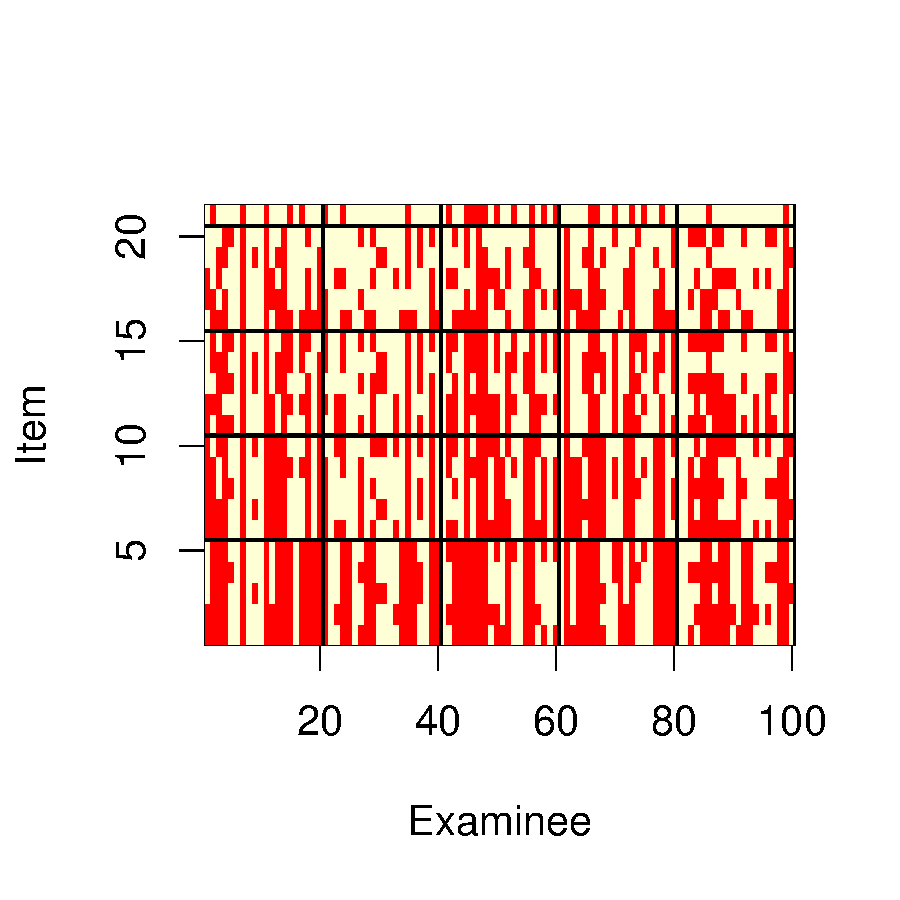
\includegraphics[scale =0.5] {ResultM}
 }
\caption{Q-matrix and an example of simulated data with this matrix.  Bright pixels represent 1's and dark red ones represent 0's.}
\label{figqmatrixandResutM}
\end{figure}

They also considered skills difficulty in the simulated data. They did not assign an item difficulty since this is already reflected by skill difficulties. They also reflected student ability in the skills mastery matrix where ability variance will show up as the variance in number of skills across examinees. The last two parameters that they considered are $\mathit{slip}$ and $\mathit{guess}$ factors which are set as constant values across items. The details of synthetic data generation for this model is given in chapter \ref{sec:Syn} since we used the same approach to generate synthetic data based on this model for assessing model fit.

Given the above framework, the process of generating simulated examinee data follows the following steps:
\begin{enumerate}
\item Assign a difficulty level to each skill.
\item Generate a random set of hypothetical examinee skills vectors based on the difficulty of each skill and the examinee\textquoteright{}s ability level. 
\item Generate simulated data based on equation \ref{eq:6} without taking into account the $\mathit{slip}$ and $\mathit{guess}$ parameters. This is referred to as the $ideal$ response pattern.
\item Randomly change the values of the generated data based on the $\mathit{slip}$ and $\mathit{guess}$ parameters. For example, with values of 0.1 and 0.2 respectively, this will result in approximately $10\%$ of the succeeded items to become failed, and $20\%$ of the failed items to become succeeded.
\end{enumerate}
The first two steps of this process are based on additive gaussian factors and follow a similar methodology to \citep{desmarais2011conditions}.

A sample of the results matrix is given in figure\ref{figqmatrixandResutM}. Examinee ability shows up as vertical patterns, whereas skills difficulty creates horizontal patterns. As expected, the mean success rate of the 2-skills items 1 to 15 is lower than the single skill items 16 to 21.



\subsection{Simulation methodology}


\citet{desmarais2012mapping} proposed a methodology to assess the NMF performance to infer a Q-matrix from simulated test data such as figure \ref{figqmatrixandResutM}'s. This methodology is conducted by comparing the predefined Q-matrix, $\mathbf{Q}$, as shown in figure \ref{figqmatrixandResutM}, with the $\hat{\mathbf{Q}}$ matrix obtained in the NMF of equation \ref{eq:6}.

As mentioned in section \ref{NMF_MODEL_ASSESS}, the negation operator is applied over the simulated test data and the NMF algorithm is carried over this data. For this experiment they used the R NMF package \citep{Gaujoux2010} and the Brunet NMF algorithm.

They defined a specific method for the quantitative comparison of the matrix $\hat{\mathbf{Q}}$ with $\mathbf{Q}$. First, the $\hat{\mathbf{Q}}$ matrix contains numerical values on a continuous scale. To simplify the comparison with matrix $\mathbf{Q}$, which is composed of \{0, 1\} values, they discretize the numerical values of $\hat{\mathbf{Q}}$ by applying a clustering algorithm to each item in $\hat{\mathbf{Q}}$, forcing two clusters, one for 0\textquoteright{}s and one for 1\textquoteright{}s. For example, item 1 in the NMF inferred matrix of figure \ref{ClusteringResults}  (which will be explained later) corresponds to a vector of six numerical values, say \{1.6, 1.7, 0.0015, 0.0022, 0.0022, 0.0018\}. This vector clearly cluster into the \{1, 1, 0, 0, 0, 0\} vector of item 1 in figure \ref{ClusteringResults}. The K-means algorithm is used for the clustering process of each item which is provided in R (version 2.13.1).

Then, to determine which skill vector (column) of the $\hat{\mathbf{Q}}$ matrix corresponds to the skill vector of the $\mathbf{Q}$ matrix, a correlation matrix is computed and the highest correlation of each column vector $\hat{\mathbf{Q}}$ is in turn matched with the corresponding unmatched column in $\mathbf{Q}$.

A visual representations of the raw and the \textquotedblleft{}discretized\textquotedblright{} (clustered) $\hat{\mathbf{Q}}$ matrix is used to provide an intuitive view of the results, as well as a quantitative measures of the fit corresponding to the average of the correlations between the matched skills vectors $\hat{\mathbf{Q}}$ and $\mathbf{Q}$.


\subsection{Results}


In order for the mean and variance of the simulated data to reflect realistic values of test data, the skill difficulty and examinee ability parameters are adjusted such that the average success rate is close to 60\%. Examinee ability is combined with the skill difficulty vectors to create a probability matrix of the same dimensions as $\mathbf{S}$, from which $\mathbf{S}$ is obtained.


\begin{figure}[!h]
\centering

\subfigure[Matrix $\hat{\mathbf{Q}}$ without slip and guess factors ($r=1$)]{
   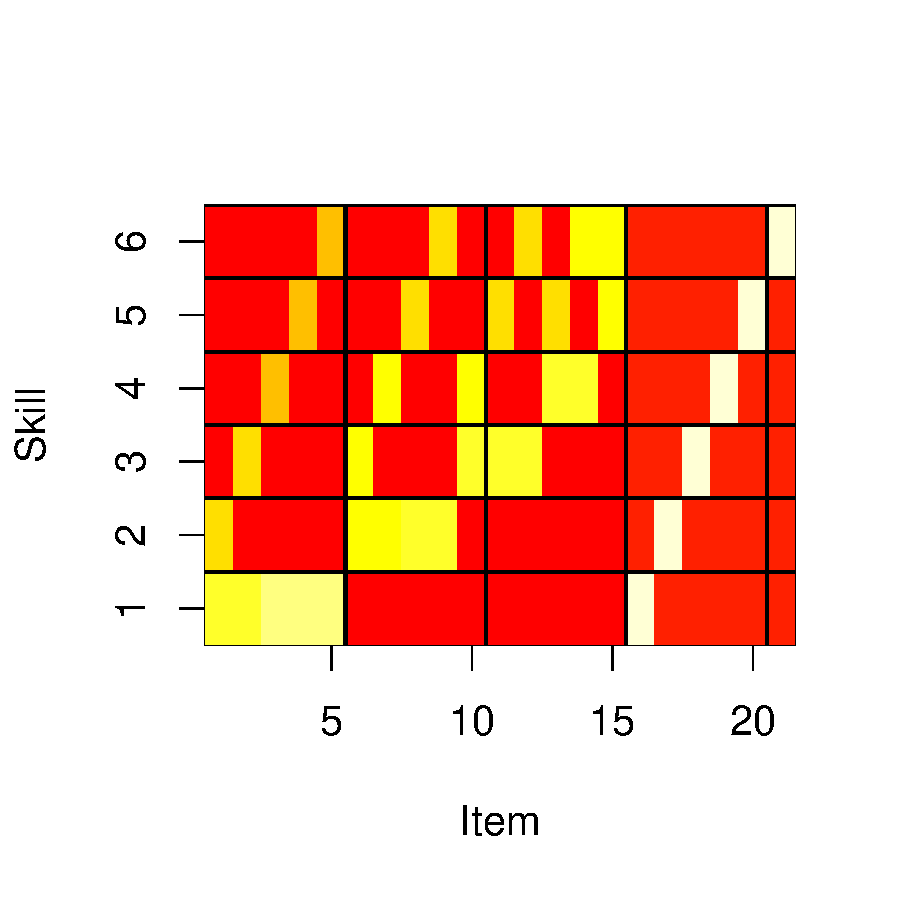
\includegraphics[scale =0.5] {NONnoiseQ}\label{NonnoisyQ}
 }\quad
 \subfigure[Discretized $\hat{\mathbf{Q}}$ without slip and guess factors ($r=1$)]{
   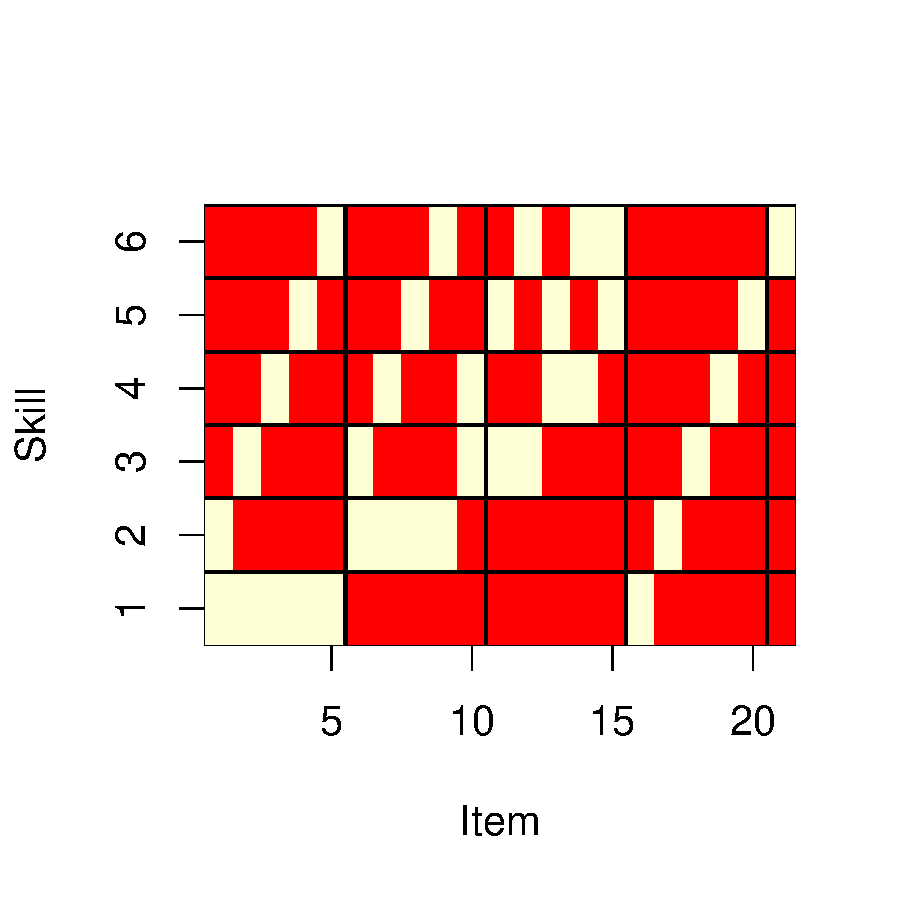
\includegraphics[scale =0.5] {ClustNONnoiseQ}\label{ClustNonnoisyQ}
 }
\centering
\subfigure[Matrix $\hat{\mathbf{Q}}$ with slip and guess factors of 0.2 ($r=0.91$)]{
   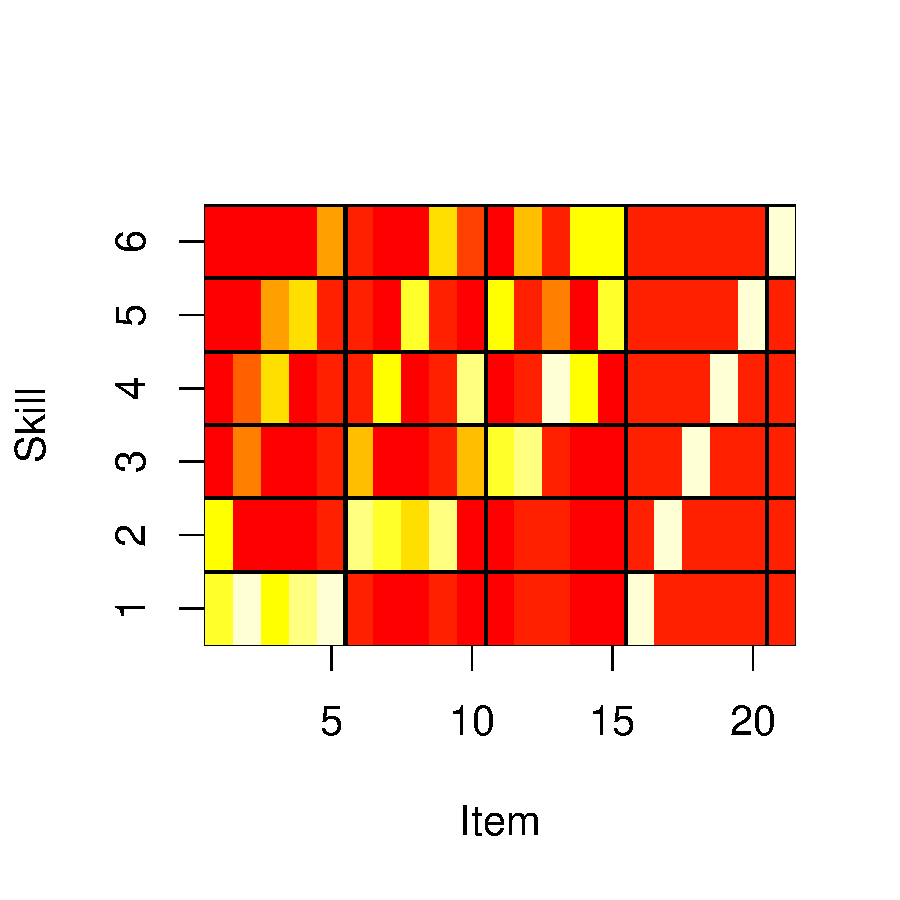
\includegraphics[scale =0.5] {noiseQ}\label{NoisyQ}
 }\quad
 \subfigure[Discretized $\hat{\mathbf{Q}}$ for slip and guess of 0.2 ($r=0.93$).  Three out of 36 skill requirements are incorrectly mapped in this example.]{
   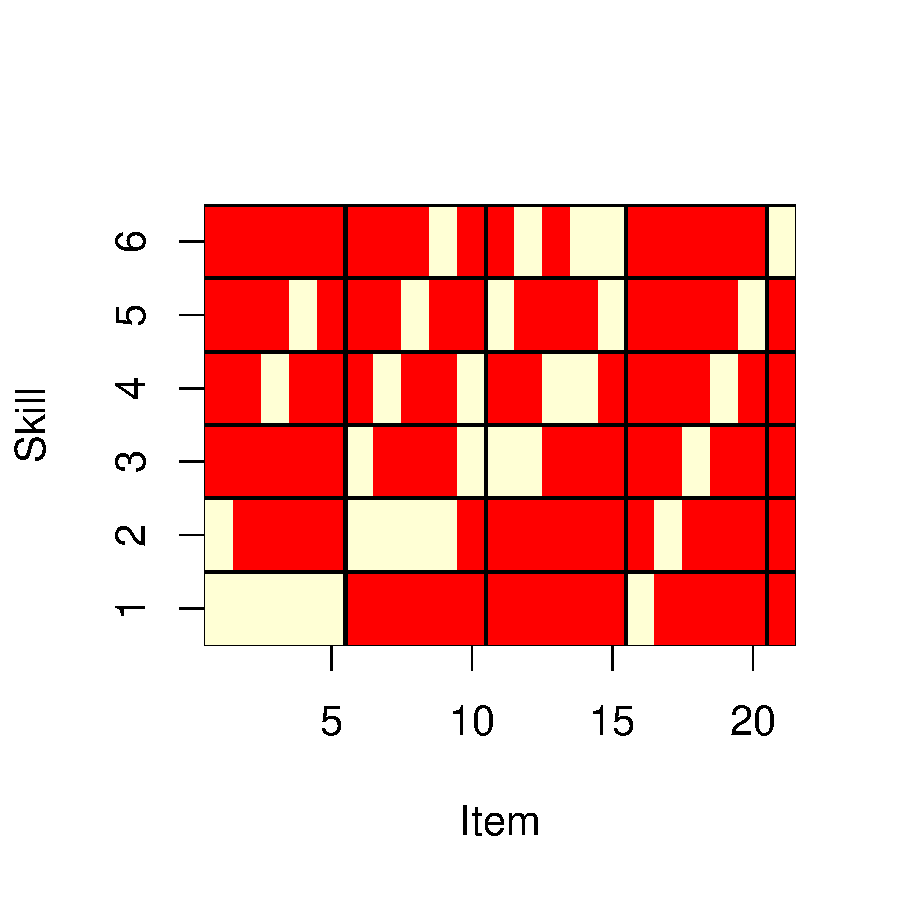
\includegraphics[scale =0.5] {ClustnoiseQ}\label{ClustNoisyQ}
 }
\caption{Visual representations of the original $\mathbf{Q}$ matrix and NMF derived matrices $\hat{\mathbf{Q}}$}
\label{ClusteringResults}
\end{figure}


Figure \ref{NonnoisyQ} shows a heat map of the matrix $\mathbf{Q}$ inferred from an ideal response pattern of 200 simulated examinees. Skill difficulties were set at (0.17, 0.30, 0.43,0.57, 0.70, 0.83) and examinee mean ability and standard deviation respectively at 0 and 0.5. The discretized version of figure \ref{NonnoisyQ}\textquoteright{}s matrix is shown in figure \ref{ClustNonnoisyQ} and it is identical to the underlying matrix $\mathbf{Q}$ in figure \ref{PerfectQ}.

Figure \ref{NonnoisyQ} and \ref{ClustNoisyQ} shows the effect of adding slip and guess parameters of 0.2 for each. The mapping to the underlying matrix $\mathbf{Q}$ degrades as expected, but remains relatively accurate.

Table \ref{tab:wq-comp} reports the results of the quantitative comparison between the $\mathbf{Q}$ matrix and the $\hat{\mathbf{Q}}$ matrix inferred as a function of different slip and guess parameters. These results are based on 10-fold simulations. The mean of the Pearson correlation coefficient (r) between $\mathbf{Q}$ and $\hat{\mathbf{Q}}$ is reported for the discretized version of $\hat{\mathbf{Q}}$ obtained with the clustering algorithm described in previous section. In addition, the error rate as computed by this formula is also provided:

\begin{equation}
  Err = \frac{\sum_{ij} |w_{ij} - q_{ij}| }{2 \cdot \sum_{ij} |q_{ij}| }
\end{equation}
Where $w_{ij}$ and $q_{ij}$ are respectively the $(i,j)$ cells of the matrices $\hat{\mathbf{Q}}$ and $\mathbf{Q}$.  The error rate will be $0$ for a perfectly matched $\mathbf{Q}$ and~$1$ when no cells match.  A value of~$0.5$ indicates that half of the non-zero cells are correctly matched. For the matrix $\mathbf{Q}$, the estimated random error rate is 71\%.

The 0 \textit{slip} and 0 \textit{guess} condition (first line) correspond to figures \ref{NonnoisyQ} and \ref{ClustNonnoisyQ}, whereas the corresponding 0.2--0.2 condition (line~3) correspond to figures\ref{NoisyQ}  and \ref{ClustNoisyQ}.



\newcommand{\ha}[2]{\multicolumn{#1}{c}{\textbf{#2}}}
\newcommand{\hb}[1]{\ha{1}{#1}}
\begin{table}
  \caption{Quantitative comparison between original $\mathbf{Q}$ matrix and NMF derived matrices $\hat{\mathbf{Q}}$.  Results are based on means and standard deviation over 10 simulation runs.}
  \begin{center}
    \newcolumntype{.}{D{.}{.}{-1}}
  \begin{tabular}{cccccc}
    \hline
 \hb{Slip} & \hb{Guess} & \hb{$\overline{r}$} & \hb{sd($\overline{r}$)} & \hb{Err} & \hb{sd(Err)} \\ 
  \hline
0.00 & 0.00 & 1.00 & 0.00 & 0.00 & 0.00 \\ 
0.10 & 0.20 & 0.97 & 0.03 & 0.02 & 0.02 \\ 
0.20 & 0.20 & 0.90 & 0.06 & 0.07 & 0.04 \\ 
0.30 & 0.20 & 0.63 & 0.08 & 0.26 & 0.06 \\ 
0.40 & 0.20 & 0.49 & 0.07 & 0.36 & 0.06 \\ 
  \hline
  \end{tabular}
  \end{center}

\label{tab:wq-comp}
\end{table}

Up to the 0.2--0.2 slip-guess condition, the skill mapping stays relatively close to perfect. On average, approximately only 2 or 3~skills requirements are wrongly assigned out of the 36 skills requirements (7\%) at the 0.2--0.2 condition.  However, the error rate increases substantially at the 0.3--0.2 slip-guess condition, and at the 0.4--0.2 condition, the quality of the match is considerably degraded with an average of 13/36 wrong assignements (36\%).

\subsection{Discussion}

The proposed approach to deriving a conjunctive Q-matrix from simulated data with NMF is successful but, as we can expect, it degrades with the amount of \textit{slips} and \textit{guesses}. If the conjunctive Q-matrix contains one or two items per skill and the noise in the data remains below slip and guess factors of~$0.2$, the approach successfully derives the Q-matrix with very few mismatches of items to skills.  However, once the data has slip and guess factors of~$0.3$ and~$0.2$, then the performance starts to degrade rapidly.

Of course, with a slip factor of~$0.3$ and a guess factor~$0.2$, half the values in the results become inconsistent with the Q-matrix. A substantial degradation is therefore not surprising.  But in this experiment with simulated data, we have a number of advantages that are lost with real data: the number of skills is known in advance, no item has more than two conjunctive skills, skills are independent, and surely other factors will arise to make real data more complex.  Therefore, we can expect that even if real data does not have a 50\% rate of inconsistent results with the examinees' skills mastery profile, other factors might make the induction of the Q-matrix subject to errors of this scale.

\section{Finding the number of latent skills}
\label{EDM2012}

We do not need to identify all the skills behind an item in order to use the item outcome for assessment purpose. As long as we can establish a minimally strong tie from an item to a skill, this is a sufficient condition to use the item in the assessment of that skill. But knowledge that there is a fixed number of determinant factors to predict item outcome is a useful information. For example, if a few number of skills, say 6, are meant to be assessed by a set of 20 questions items, and we find that the underlying number of determinant latent factors behind these items is very different than 6, then it gives us a hint that our 6-skills model may not be congruent with the assessment result.

In an effort towards the goal of finding the skills behind a set of items, we investigate two techniques to determine the number of dominant latent skills. The SVD is a known technique to find latent factors. The singular values represent direct evidence of the strength of latent factors. Application of SVD to finding the number of latent skills is explored. We introduce a second technique based on a wrap- per approach. Linear models with different number of skills are built, and the one that yields the best prediction accuracy through cross validation is considered the most appropriate. The results show that both techniques are effective in identifying the latent factors over synthetic data. An investigation with real data from the fraction algebra domain is also reported. Both the SVD and wrapper methods yield results that have no simple interpretation.


\subsection{SVD-Based method}

SVD is a well known matrix factorization technique that decomposes any matrix, $\mathbf{A}$, into three sub-matrices: 

\begin{equation}
\mathbf{A}=\mathbf{UDV^{T}}\label{eq:SVD}
\end{equation}


where $\mathbf{U}$ and $\mathbf{V}$ are orthonormal matrices and their column vectors respectively represent the eigenvectors of $\mathbf{\mathbf{A}A^{T}}$ and $\mathbf{A^{T}\mathbf{A}}$. $\mathbf{D}$ is a diagonal matrix that contains the singular values. They are the square root of the eigenvalues of the eigenvectors and are sorted in a descending order. Because the singular values represent scaling factors of the unit eigenvectors in equation \ref{eq:SVD}, they are particularly useful in finding latent factors that are dominant in the data. This is demonstrated with simulated data below. The simulated data in this experiment is generated based on the same pattern on the previous section. Again we have all combination of skills for items, at most 2 skills per item and all other factors like slip and guess.


\subsection{Wrapper-Based method}


We introduce a second method to determine the number of dominant skills behind items based on a wrapper approach. In statistical learning, the wrapper approach refers to a general method for selecting the most effective set of variables by measuring the predictive performance of a model with each variables set (see \citep{Guyon2003}). In our context, we assess the predictive performance of linear models embedding different number of latent skills. The model that yields the best predictive performance is deemed to reflect the optimal number of skills.

The wrapper method requires a model that will predict item outcome. A linear model of skills is defined for that purpose on the basis of the equation \ref{eq:1}. This model represents a compensatory interpretation of skills modelling, where each skill contributes additively to the success of an item. The conjunctive model of skills was presented in \ref{eq:6}. To estimate the optimal number of skills, the wrapper model can either correspond to equation\ref{eq:1} or \ref{eq:6}. We will focus our explanations around equation \ref{eq:1}, but they obviously apply to \ref{eq:6} if $\mathbf{R}$ and $\mathbf{S}$ are negated.

This model states that, given estimates of $\mathbf{Q}$ and $\mathbf{S}$, we can predict $\mathbf{R}$. We refer to these estimates as $\hat{\mathbf{Q}}$ and $\hat{\mathbf{S}}$, and to the predictions as $\hat{\mathbf{R}}=\hat{\mathbf{Q}}\hat{\mathbf{S}}$. The goal is therefore to derive estimates of $\hat{\mathbf{Q}}$ and $\hat{\mathbf{S}}$ with different number of skills and measure the residual difference between $\mathbf{R}$ and $\hat{\mathbf{R}}$. 

First, $\hat{\mathbf{Q}}$ is learned from an independent set of training data. Then, $\hat{\mathbf{S}}$ is learned from the test data, and the residuals are computed%
\footnote{Note that computing $\hat{\mathbf{S}}$ from the test data raises the issue of over-fitting, which would keep the accuracy growing with the number of skills regardless of the \textquotedblleft{}real\textquotedblright{} number of skills. However, this issue is mitigated by using independent learning data for $\hat{\mathbf{Q}}$ , without which, we empirically observed, the results would deceive us: in our experiments using both $\mathbf{Q}$ and $\mathbf{S}$ from NMF while increasing the rank of the factorization (number of skills), ends up increasing prediction accuracy even after we reach beyond the \textquotedblleft{}real\textquotedblright{} number of skills. This can reasonably be attributed to over-fitting. %
}.

An estimate of $\hat{\mathbf{Q}}$ is obtained through NMF. Details on applying this technique to the problem of deriving a Q-matrix from data is found in \citep{desmarais2011conditions} and we limit our description to the basic principles and issues here.

The NMF technique requires to choose a rank for the decomposition, which corresponds in our situation to the number of skills (i.e. number of columns of $\mathbf{Q}$ and number of rows of $\mathbf{S}$). Because NMF constrains $\mathbf{Q}$ and $\mathbf{S}$ to non-negative values, their respective interpretation as a Q-matrix and a as student skills assessments is much more natural than other matrix factorization techniques such as Principal Component Analysis, for example. However, multiple solutions exists to this factorization and there are many algorithms that can further constrain solutions, namely to force sparse matrices. Our experiment relies on the R package named NMF and the Brunet algorithm \citep{Gaujoux2010}.

Once $\hat{\mathbf{Q}}$ is obtained, then the values of $\hat{\mathbf{S}}$ can be computed through linear regression. Starting with the overdetermined system of linear equations:

\begin{equation}
\mathbf{R}=\hat{\mathbf{Q}}\hat{\mathbf{S}}\label{eq:Estimation}
\end{equation}


which has the same form as the more familiar $y=\mathbf{X}\beta$ (except that $y$ and $\beta$ are generally vectors instead of matrices), it follows that the linear least squares estimate is given by:

\begin{equation}
\hat{\mathbf{S}}=\left(\hat{\mathbf{Q}}^{T}\hat{\mathbf{Q}}\right)^{-1}\hat{\mathbf{Q}}^{T}\mathbf{R}\label{eq:ShatEstimation}
\end{equation}


Equation \ref{eq:ShatEstimation} represents a linear regression solution which minimizes the residual errors $\left(\left\Vert \mathbf{R}-\hat{\mathbf{Q}}\hat{\mathbf{S}}\right\Vert \right)$.

\subsection{Results of SVD-Based method}


The results of the SVD method are shown in figure \ref{SVD-simul}. The x is the index of the singular value, and the y axis is its actual value. Recall that the singular values of SVD indicate the strength of latent factors.

Three conditions are reported in figure \ref{SVD-simul}. The y values at 1 on the x scale are truncated on the graph to allow a better view of the interesting region of the graph, but the highest value is from the {[}guess=0, slip=0{]} condition and the lowest is for the random condition. The random curve condition can be obtained by simulating random \{0, 1\} values and ensuring that the overall average score of the results matrix reflects the original's data average. In this random condition, the slope from singular value 2 to 21 remains relatively constant, suggesting no specific number of skills. In condition {[}guess=0, slip=0{]}, a sharp drop occurs between singular values of 6 and 7. Then the slope remains relatively constant from values 8 to 21. The largest drop is clearly at value 6 which corresponds to the underlying number of skills. In the third condition {[}guess=0.2, slip=0.1{]}, the largest drop still remains visible between 6 and 7, but not as sharp as for the noiseless condition,
as expected.

In other experiments with various number of skills, not reported here due to space constraints, we observed similar patterns. Another observation is that the random curve intersects with the other two after the number of underlying latent skills (after 6 in figure \ref{SVD-simul}'s experiment).

Therefore, the SVD method does allow for the identification of the number of skills with synthetic data, at least up to the {[}guess=0.2, slip=0.1{]} level.

\begin{figure}
\centering
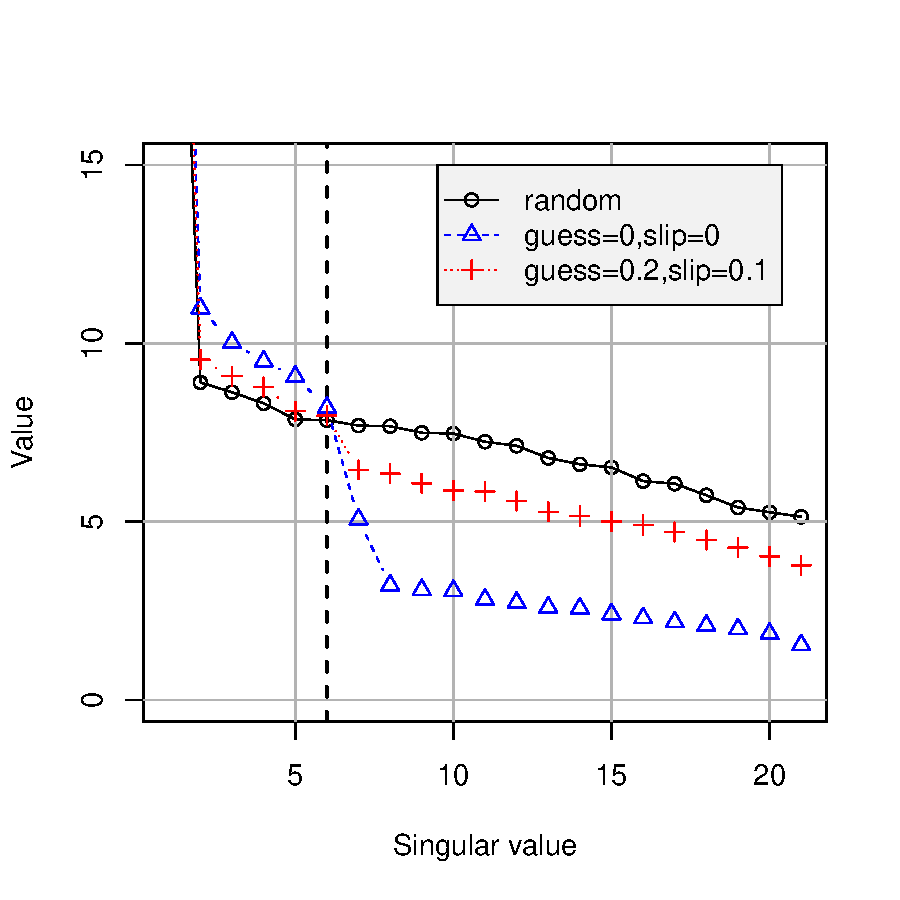
\includegraphics[scale=0.6]{svd-simul}\caption{Singular values of simulated data for a 21 items test. A vertical
dashed line at singular value 6 corresponds to the number of underlying
latent skill factors.}
\label{SVD-simul}

\end{figure}

\subsection{Results of Wrapper-Based method}


We would expect the model with the correct number of skills to perform the best, and models with fewer skills to under- perform because they lack the correct number of latent skills to reflect the response patterns. Models with greater number of skills than required should match the performance of the correct number model, since they have more representative power than needed, but they run higher risk of over- fitting the data and could therefore potentially show lower accuracy in a cross-validation. However, the skills matrix $\hat{\mathbf{S}}$ obtained through equation \ref{eq:ShatEstimation} on the test data could also result in over-fitting that will increase accuracy this time.

Figure \ref{Wrapper} shows the percentage of correct predictions of the models as a function of the number of skills. Given that predictions are \{0,1\}, the percentage can be computed as $\left(\left\Vert \mathbf{R}-\hat{\mathbf{Q}}\hat{\mathbf{S}}\right\Vert \right)/mn$, where m and n are the number of rows and columns of $\mathbf{R}$.

\begin{figure}
\centering

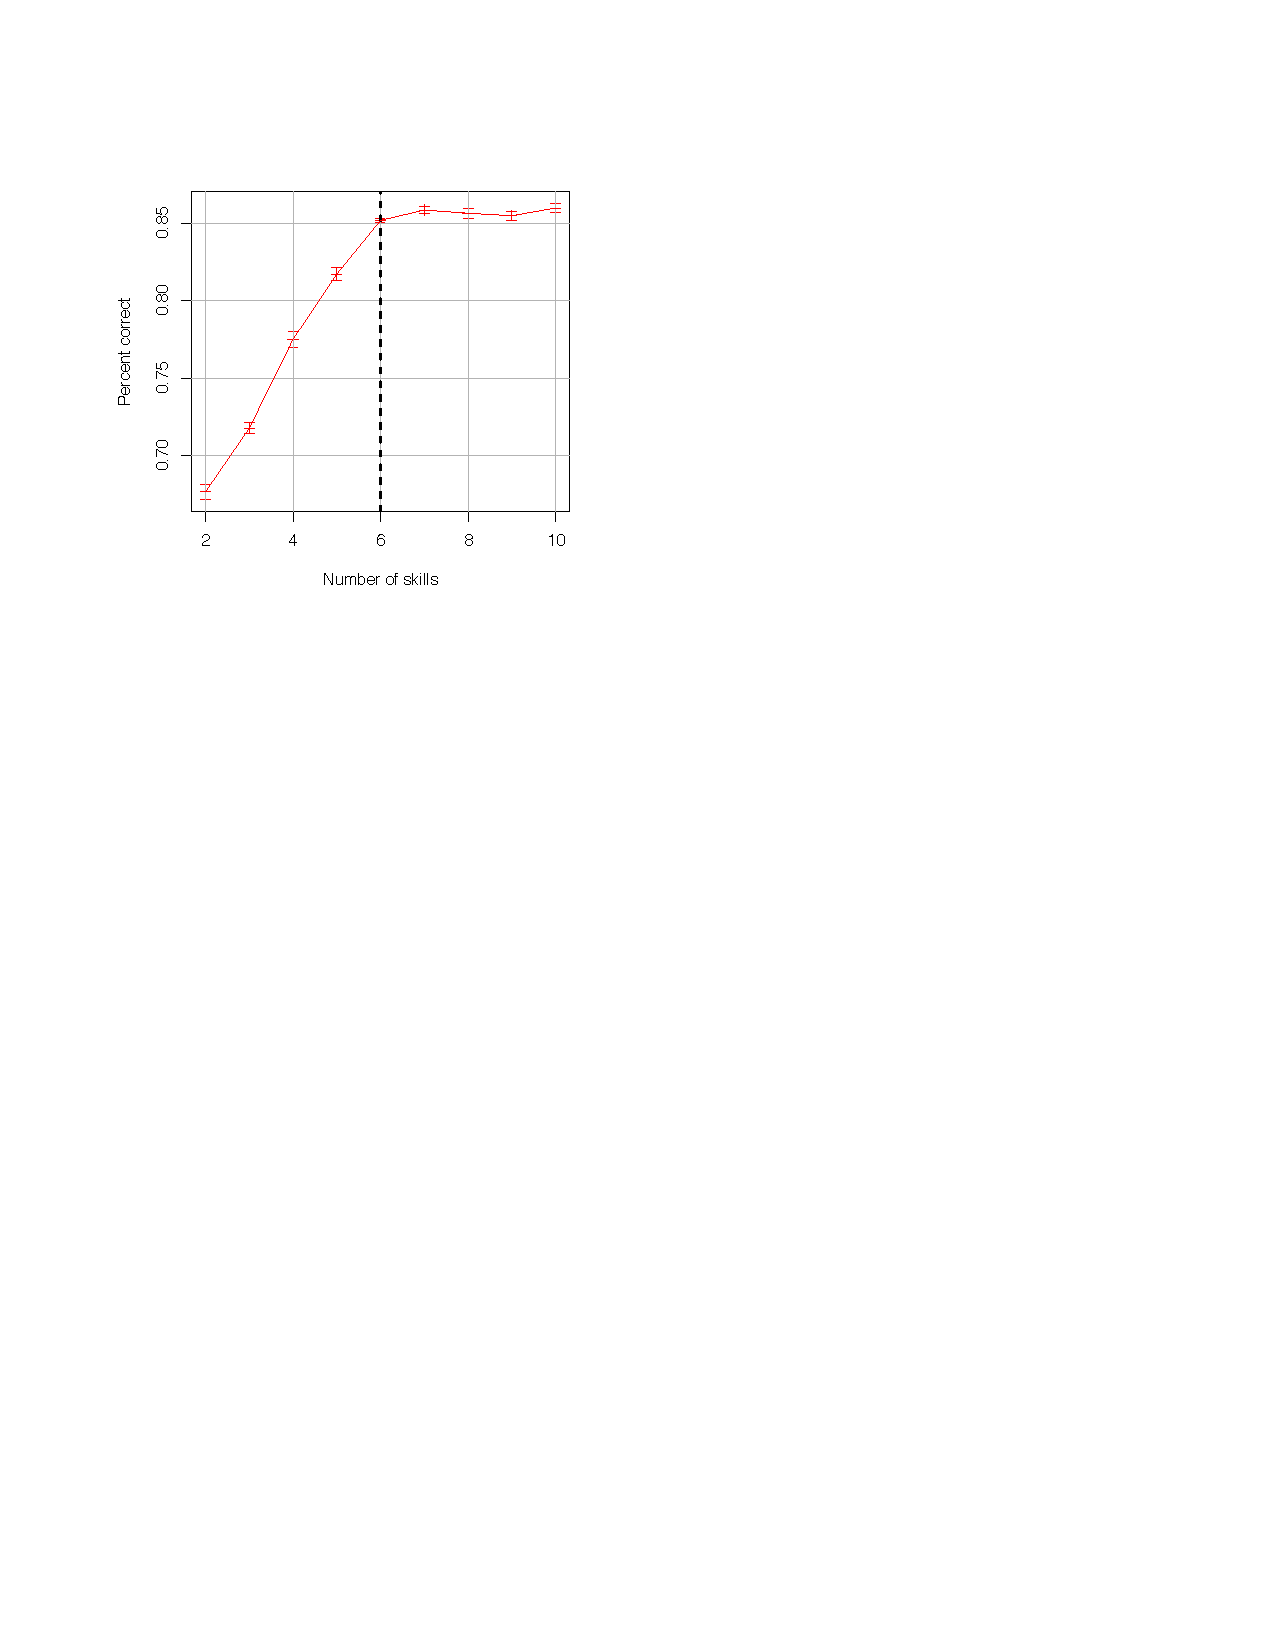
\includegraphics{Wrapper}\caption{Precision of student results predictions from estimated skill matrix
(equation \ref{eq:ShatEstimation}). Error bars are the standard error
of the accuracy curves. Experiment is done with simulated data with
6 skills and slip and guess values of 0.1 and 0.2 respectively.}
\label{Wrapper}
\end{figure}


The results confirm the conjectures above: the predictive accuracy increases until the underlying number of skills is reached, and it almost stabilizes thereafter. Over-fitting of $\hat{\mathbf{S}}$ with the test data is apparently not substantial. It is interesting to note that the accuracy increments of figure \ref{Wrapper} are relatively constant between each skill up to 6. This is also what we would expect since every skill in the underlying Q-matrix has an equivalent weight to all others. We expect that differences in increments indicate differences in the weights of the skills. This could either stem from the structure of the Q-matrix (for e.g., more items can depend on one skill than on another), or on the criticality of the skill over its item outcome.



\subsection{Discussion}
This research showed that Both the SVD and the wrapper methods provide strong cues of the number of underlying skills with simulated student test data.  However, for the Vomlel data set, both methods yield results that are much more ambiguous.  Instead of the 7~skills that were identified by experts over the 17~items set, the SVD method suggests only 2~skills if we rely on the intersection with the random data curve, and no clear number if we look for a change of slope after skill~2.  The wrapper method shows data that is also consistent with 2~skills to the extent that a drop of accuracy is observed at 3~skills, but a rise of accuracy up to 8~skill draws an interpretation closer to the experts' 7 skills set.

An important difference between the SVD and the wrapper methods has to do with the independence of skills.  For SVD, orthogonality of the singular matrices $\mathbf{U}$ and $\mathbf{V}$ in equation~(\ref{eq:1}) forces latent factors to be independent.  NMF does not require latent factors to be independent.  The orthogonality constraint of may limit the application of the SVD method with respect to real skills and might explain some of the difference between the two methods.  The skills from the synthetic data of the first experiment were independent and the Q-matrix had an homogeneous pattern for each skill, and therefore the effect of dependence between skills could not come into play.

Obviously, the study calls for more investigations.  The findings from one set of data from the real world may be highly different from another set. More studies should be conducted to assess the generality of the findings.  Other investigations are called for to find ways to improve these methods and to better understand their limits when faced with real data.  In particular, we need to know at which level of noise from guess and slip factors do the methods break down, and what is the ratio of latent skills to data set size that is critical to avoid over-fitting of the wrapper method.

One improvement that can be brought to the wrapper method is to use a cross validation to derive the skills matrix.  This would require the use of two sets of items, one for testing and one for assessing the student's skills.  This comes at the cost of a greater number of items, but it avoids the problem of over-fitting that leads to accuracy increases.

\section{The refinement of a Q-matrix}
\label{edm2014}

Validating of the expert defined Q-matrix has been the focus of recent developments in the field of educational data mining in recent years \citep{delaTorre2008,chiu2013statistical,barnes2010novel,loye2011validite,Desmarais2013aied}.
In this section we compare three data driven techniques for the validation of skills-to-tasks mappings.  All methods start from a given expert defined Q-matrix, and use optimization techniques to suggest a refined version of the skills-to-task mapping.  
%To validate the different techniques, we inject alterations in the Q-matrix and verify whether the original Q-matrix can be recovered.  Tests are run over both simulated and real data.  The comparison of the techniques over ten data sets shows that, in general, around 1/2 to 2/3 of the alterations can be restored to their original values by the best performer, the ALS matrix factorization method, but the results vary substantially across techniques, and across data sets.


%%%%%%%%%%%%%%%%%%%%%%%%%%%%%%%%%%%%%%%%%%%%%%%%%%%%%%%%%%%%%%%%%%%%%%%%%%%%%
\subsection{Q-matrices validation techniques}

Two techniques for Q-matrix validation surveyed here rely on the DINA and DINO models, whereas one relies on a matrix factorization technique called ALS.  We briefly review each technique below before describing the experiments.


%%%%%%%%%%%%%%%%%%%%%%%%%%%%%%%%%%%%%%%%%%%%%%%%%%%%%%%%%%%%%%%%%%%%%%%%%%%%%
\begin{description}


\item[de~la Torre (2008)] The method defined by \citet{delaTorre2008} searches for a Q-matrix that maximizes the difference in the probabilities of a correct response to an item between examinees who possess all the skills required for a correct response to that item and examinees who do not. It first uses the DINA model and an EM algorithm to estimate the slip and guess parameters, after which it can calculate the respective probabilities.  The difference between the two probabilities represents an item discrimination index: the greater the difference between the probability of a correct response given the skills required to the probability given missing skills, the greater the item is discriminant. Therefore we can consider that the method finds a Q-matrix that maximizes item discrimination over all items.

%%%%%%%%%%%%%%%%%%%%%%%%%%%%%%%%%%%%%%%%%%%%%%%%%%%%%%%%%%%%%%%%%%%%%%%%%%%%%

\item[Chiu (2013)] Chiu defines a method that minimizes the residual sum of square (RSS) between the real responses and the ideal responses that follow from a given Q-matrix~\citep{chiu2013statistical}.  The algorithm adjusts the Q-matrix by choosing the item with the worst RSS over to the data, and replaces it with the one has the lowest RSS, and iterates until convergence.

%%%%%%%%%%%%%%%%%%%%%%%%%%%%%%%%%%%%%%%%%%%%%%%%%%%%%%%%%%%%%%%%%%%%%%%%%%%%%
\item[ALS] The  (ALS) method is defined in \citep{Desmarais2013aied}.  Contrary to the other two methods, it does not rely on the DINA model.  Instead, it decomposes the results matrix $\mathbf{R}_{m \times n}$ of~$m$ items by~$n$ students as the inner product two smaller matrices:

\begin{equation}
  \mathbf{{R}} = \mathbf{Q} \, \mathbf{S} \label{eq:nmf}
\end{equation}

where $\mathbf{R}$ is the results matrix ($m$~items by $n$~students),  $\mathbf{Q}$ is the $m$~items by $k$~skillls Q-matrix, and~$\mathbf{S}$ is the mastery matrix of $k$~skills by $n$~students.

\end{description}
%%%%%%%%%%%%%%%%%%%%%%%%%%%%%%%%%%%%%%%%%%%%%%%%%%%%%%%%%%%%%%%%%%%%%%%%%%%%%
\subsection{Methodology and data sets}

\begin{table*}[ht]
\begin{center}
  \caption{\protect\raisebox{0pt}[0pt][6pt]{Data sets}}
  \label{tab:datasets}
  \begin{tabular}{|llccc p{7.75cm} |}
  \hline
  \multicolumn{2}{|c}{\multirow{2}{*}{\textbf{Name}}} & \multicolumn{3}{c}{\bf Number of}  & \multicolumn{1}{c|}{\multirow{2}{*}{\textbf{Description}}}\tabularnewline

  \cline{3-5}
&   & \multicolumn{1}{c@{~~}}{\bf \raisebox{0pt}[12pt][6pt]{Skills}} &
  \multicolumn{1}{@{}c}{\bf Items} &
  \multicolumn{1}{@{~~~}c@{~~~}}{\bf Cases} & \\
  \hline
%\newcounter{exone}\setcounter{exone}{\thei}\refstepcounter{exone}\label{lab:exone} % allows to use ref/label mechanism (although for some reason it has to be above the reference before).
 1. &  Sim. DINA & 3 & 9 & 400 & {Artificial data available from
    the (\texttt{sim.dina}) data set of the CDM package.
  %% Generated with the DINA model.  The slipping errors vary from 0.0 to 0.3. The attributes
  %% are assumed to be mastered with expected probabilities of -0.4 , 0.2, 0.6,
  %% respectively. The correlation of the attributes is 0.3 for attributes 1 and 2, 0.4 for
  %% attributes 1 and 3 and 0.1 for attributes 2 and 3.
} 
\\
  \hline
2. &  Sim. DINO & 3 & 9 & 400 & {Same parameters as No.~1 but using the
    DINO model (\texttt{sim.dino} data set).} \\  
  \hline
3. &  \parbox{2cm}{\raggedright Sim. CDM DINA} & 3 & 12 & 4000 & {Artificial data generated through the
  CDM function \texttt{sim.din}}.\\
  \hline
4. &  Sim. DCM & 3 & 7 & 10000 & {Artificial data from chapter 9 of the book \textit{Diagnostic Measurement} \cite{rupp2010diagnostic}} \\  
  \hline
5. &  ECPE & 3 & 28 & 2922 & {Dataset from \cite{templin2013obtaining} in \cite{torre2009dina}} \\  
  \hline
6. &  Fraction & 8 & 20 & 536 & {Tatsuoka's fraction algebra
problems~\cite{Tatsuoka1984analysis} (see table~1 in~\cite{DeCarlo2011} for a description of the problems
and of the skills). } \\  
  \hline
7. &  Fraction 1 & 5 & 15 & 536 & {15 questions subset of Fraction
    with Q-matrix defined in \cite{torre2009dina}.} \\  
  \hline
8. &  Fraction 2/1 & 3 & 11 & 536 & {11 questions subset of Fraction
    with Q-matrix from \cite{henson2009defining}.} \\  
  \hline
9. &  Fraction 2/2 & 5 & 11 & 536 & {11 questions subset of Fraction
    with Q-matrix from \cite{torre2009dina}.} \\  
  \hline
10. &  Fraction 2/3 & 3 & 11 & 536 & {3 skills version of Fraction~1.} \\  
  \hline
  \end{tabular}
\end{center}
\end{table*}
%% How many changes are suggested by each technique?
%% What about DINO models of the other techniques?

The two first methods, de~la Torre (2008)~\citep{delaTorre2008} and Chiu (2013)~\citep{chiu2013statistical}, have been shown to perform well on artificial data.  On real data, the performance is more blurry.  The ALS factorization method \citep{Desmarais2013aied} has only been tested on one real data set.  But the methodologies used to validate all three techniques in each respective study vary considerably and do not allow for a proper comparison.

To validate and compare the effectiveness of each technique for refining a given Q-matrix, we follow a methodology based on recovering the Q-matrix from a number perturbations: the binary value of a number of cells of the Q-matrix is inverted, and this ``corrupted'' matrix is given as input to each technique.  If the technique recovers the original value of each altered cell, then we consider that it successfully ``refined'' the Q-matrix.

A total of 30 perturbations are randomly injected in each Q-matrices to validate a method's capacity to recover the original matrix.  Note that when a single perturbation is injected, the maximum number of different perturbations is the size of the Q-matrix. Therefore, if is the size of the Q-matrix is smaller than~30, the total number of perturbations is limited to the number of cells in the Q-matrix.

The experiment is repeated for each of the 10~levels of perturbation, and for each of the 10~data sets described later.  This set of experiments is referred to as a single run, and performance measures are averaged over 8~runs.

The measures of performance are the number of \textit{true positives} and \textit{false positives}:
\begin{itemize}
\item \textbf{Mean true positives}: a \textit{true prositive} corresponds to an alteration that was injected in the input, and was correctly switched back to its original value by the method. The measure reported is the number of correctly recovered alterations averaged over the 8~runs. 
\item \textbf{Mean false positive ratio}: a \textit{false positive} corresponds to a changed Q-matrix entry returned by the method, but that was not injected in the input.  Hereto the mean over all perturbation runs is given.
\end{itemize}

For real data, this methodology rests on the assumption that the original matrix is better than the corrupted one, which is not necessarily the case with an expert generated Q-matrix. The expert may be wrong.  However, we have no other means to inform us of the ``real'' Q-matrix and it is reasonable to assume that most of the cells in the Q-matrix are correct.

For synthetic data, this assumption is correct as the Q-matrix is at the source of the generation of the data, but, of course, the model behind the process may not be a reliable reflection of the real cognitive processes involved.  

A total of 10~data sets are used for the validation.  They are freely available from two R~packages: CDM (\url{http://cran.r-project.org/web/packages/CDM/index.html}) \citep{Robitzsch2012} and Chiu (2013) (\url{http://cran.r-project.org/web/packages/NPCD/NPCD.pdf}).  Table~\ref{tab:datasets} contains a short description of each data set.  Note that for the last six data sets, the source data is the same, but different Q-matrices are defined over them and subsets of items are used in the last four: the fraction data set data is used to create four variations through subsets of questions and alternative Q-matrices (Fraction~1, Fraction~2/1, Fraction~2/2, and Fraction~2/3).  The artificial data sets are generated from the well known DINA and DINO models.

For obtaining the results of the de~la Torre (2008) method, we used the R~implementation found in the CDM package~\citep{Robitzsch2012}.  A DINA model and parameter estimation is first built with the default arguments to the \texttt{din} function, and fed to the \texttt{din.validate.qmatrix} function to obtain a refined version of the Q-matrix. For the results of the Chiu (2013) method, the R~NPCD packaged is used (function \texttt{Qrefine}).

\begin{figure*}
\subfigure[{Average recovery rate by number of perturbations (real data)}]{
  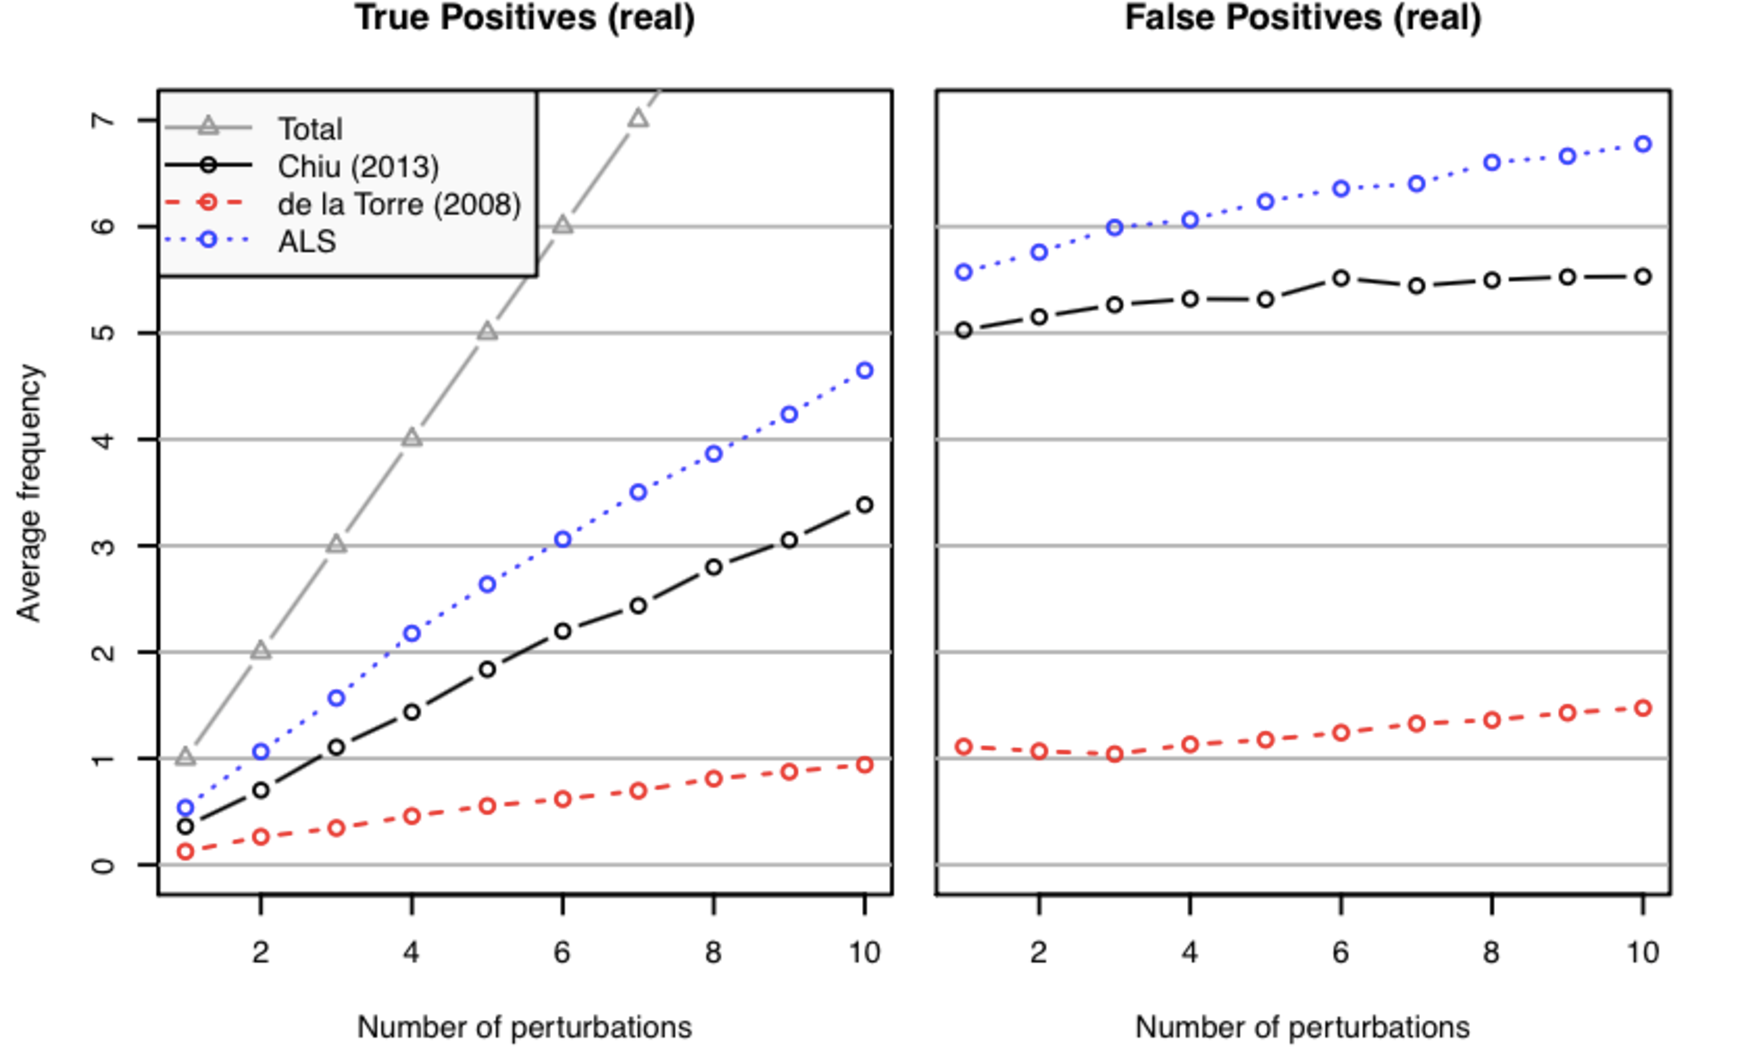
\includegraphics[width=\textwidth]{Images/average-recov.pdf}
  \label{fig:average-recov}
}
\subfigure[{Average recovery rate by number of perturbations (synthetic data)}]{
  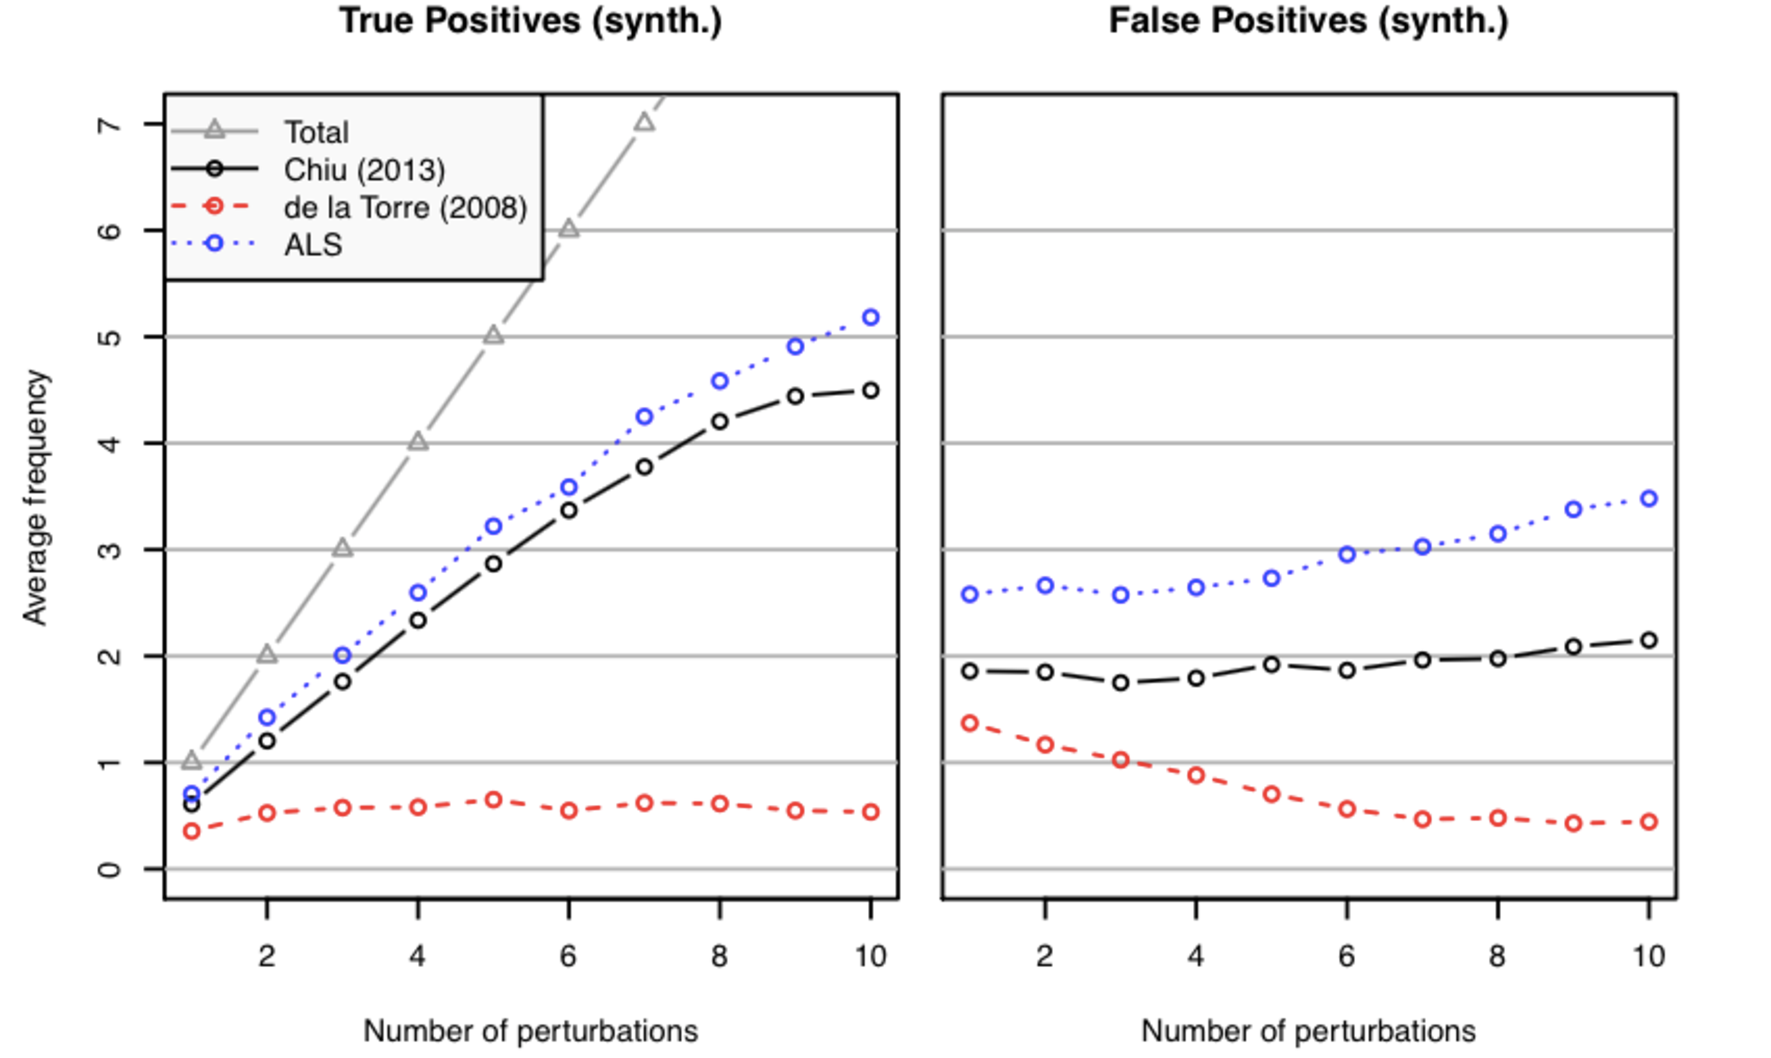
\includegraphics[width=\textwidth]{Images/average-recov-synth.pdf}
  \label{fig:average-recov-synth}
}
  \caption{Average recovery rate by number of perturbations (real and synthetic data). }
\end{figure*}

\begin{sidewaystable} 
  \caption{\protect\raisebox{0pt}[0pt][6pt]{Results by individual data set at 1 and 4 perturbations}}
%  \caption{Single perturbation results}
  \label{tab:details}
\centering
\begin{tabular}{lrrrrrrrrr}
  \hline
  \hline
\raisebox{0pt}[12pt]{~}  & \multicolumn{2}{c}{\textbf{Mean True Positives}} && \multicolumn{2}{c}{\textbf{Mean False Positives}} && \multicolumn{3}{c}{\textbf{TP/FP}}\\
  \cline{2-3} \cline{5-6} \cline{8-10}
\raisebox{0pt}[12pt]{~}   
& \multicolumn{1}{c}{\textbf{ALS}} 
& \multicolumn{1}{c}{\textbf{Chiu (2013)}} 
&
& \multicolumn{1}{c}{\textbf{ALS}} 
& \multicolumn{1}{c}{\textbf{Chiu (2013)}} 
&
& \multicolumn{1}{c}{\textbf{ALS}} 
& \multicolumn{1}{c}{\textbf{Chiu (2013)}} 
& \multicolumn{1}{c}{\textbf{Ratio}} 
\\
  \hline
  \hline
  \multicolumn{2}{l}{\raisebox{0pt}[10pt][6pt]{\textit{Synthetic @ 1 perturbation}}}\\ 
  Sim. DINA & 0.70 (0.00) & 0.55 (0.05) && 2.15 (0.00) & 0.28 (0.05) && 0.33 & 1.95 & 0.3\\ 
  Sim. DINO & 0.48 (0.00) & 0.28 (0.03) && 5.59 (0.00) & 5.30 (0.17) &&  0.09 & 0.05 & 1.8\\ 
  Sim. CDM DINA & 0.93 (0.01) & 1.00 (0.00) && 0.00 (0.00) & 0.00 (0.00) && $\infty$ & $\infty$ & -\\ 
  Sim. DCM & 0.43 (0.00) & 0.14 (0.00) && 0.00 (0.00) & 0.16 (0.02)  && $\infty$ & 0.89 &  $\infty$\\ 
  \hline
  \multicolumn{2}{l}{\raisebox{0pt}[10pt][6pt]{\textit{Real data @ 1 perturbation}}}\\
  ECPE & 0.65 (0.05) & 0.36 (0.03) && 9.81 (0.18) & 17.81 (0.16) && 0.07 & 0.02 & 3.5\\ 
  Fraction & 0.56 (0.07) & 0.46 (0.06) && 5.83 (0.19) & 2.20 (0.27) &&  0.10& 0.21 & 0.5\\ 
  Fraction 1 & 0.65 (0.05) & 0.49 (0.08) && 5.25 (0.17) & 3.14 (0.27) &&  0.12 & 0.16 & 0.8\\ 
  Fraction 2/1 & 0.52 (0.03) & 0.42 (0.03) && 4.56 (0.09) & 5.92 (0.12) &&  0.11 & 0.07 & 1.6\\ 
  Fraction 2/2 & 0.61 (0.09) & 0.41 (0.04) && 4.14 (0.18) & 0.59 (0.12) &&  0.15 & 0.71 & 0.2\\ 
  Fraction 2/3 & 0.36 (0.02) & 0.23 (0.04) && 9.39 (0.07) & 5.37 (0.20) &&  0.04 & 0.04 & 1.0\\ 

  \hline
  \hline
  \multicolumn{2}{l}{\raisebox{0pt}[10pt][6pt]{\textit{Synthetic @ 4 perturbations}}}\\
  Sim. DINA     & 2.55 (0.23) & 1.88 (0.19) && 2.55 (0.34) &  0.95 (0.28) && 1.00 & 1.99 & 0.5\\ 
  Sim. DINO     & 1.69 (0.15) & 1.12 (0.13) && 5.21 (0.19) &  4.43 (0.19) && 0.32 & 0.25 & 1.3\\
  Sim. CDM DINA & 3.57 (0.11) & 4.00 (0.00) && 0.18 (0.07) &  0.00 (0.00) &&19.75 &  Inf & 0.0\\ 
  DCM           & 2.15 (0.25) & 0.53 (0.13) && 1.01 (0.13) &  0.57 (0.12) && 2.13 & 0.94 & 2.3\\ 
  \hline
  \multicolumn{2}{l}{\raisebox{0pt}[10pt][6pt]{\textit{Real data @ 4 perturbations}}}\\
  ECPE          & 2.47 (0.23) & 1.49 (0.21) &&10.59 (0.32) & 17.35 (0.20) && 0.23 & 0.09 & 2.5\\ 
  Fraction      & 2.28 (0.14) & 1.86 (0.15) && 7.93 (0.29) &  2.74 (0.23) && 0.29 & 0.68 & 0.4\\ 
  Fraction 1    & 2.56 (0.08) & 1.95 (0.25) && 5.48 (0.25) &  3.98 (0.23) && 0.47 & 0.49 & 1.9\\ 
  Fraction 2/1  & 2.19 (0.22) & 1.80 (0.20) && 4.92 (0.27) &  5.30 (0.28) && 0.44 & 0.34 & 1.3\\ 
  Fraction 2/2  & 1.90 (0.17) & 1.04 (0.16) && 4.32 (0.35) &  1.91 (0.28) && 0.44 & 0.54 & 0.8\\ 
  Fraction 2/3  & 1.69 (0.15) & 1.41 (0.13) && 8.20 (0.23) &  5.40 (0.24) && 0.21 & 0.26 & 0.8\\ 
  \hline
  \hline
\end{tabular}
\end{sidewaystable} 

%%%%%%%%%%%%%%%%%%%%%%%%%%%%%%%%%%%%%%%%%%%%%%%%%%%%%%%%%%%%%%%%%%%%%%%%%%%%%
\subsection{Results}

The three methods are evaluated over the ten data sets and for ten runs.  Each run is conducted over a set of 30~different random combinations of perturbations, from 1~up to 10~perturbations.  For the 1-perturbation condition, the total number of possible combinations is the size of the Q-matrix itself.

%%%%%%%%%%%%%%%%%%%%%%%%%%%%%%%%%%%%%%%%%%%%%%%%%%%%%%%%%%%%%%%%%%%%%%%%%%%%%
\subsection{Recovery rates by the number perturbation}

Figure~\ref{fig:average-recov} shows the average recovery rate of each method as a function of the number of perturbations.
Recoveries are labeled ``True Positives''~(TP) whereas changes introduced by a method, but which do not correspond to perturbations,
are labeled ``False Positives''~(FP).  The top two graphs show the averages of the 6~real data sets, whereas the bottom graphs show
the averages for the 4~synthetic data sets.  Averages are computed over the 30~perturbations runs (or less if the Q-matrix has
fewer cells).  The ``Total'' line is shown to visually indicate the maximum that can be reached by a TP curve.

The ALS method shows the greatest ability to recover alterations, but at the cost of a higher rate of FP: changes
that do not correspond to perturbations.  It is followed closely by the Chiu (2013) method.  The de~la Torre (2008) method has a very low
rate of recovery (TP) that make it impractical. In general, the ALS and Chiu (2013) methods recover about~2/3 of the
perturbations for synthetic data, and this rate falls to~1/2 for real data with ALS, and about~1/3 for Chiu (2013).  For real
data, the number of FP is around~5 for Chiu (2013) and around~6 for ALS, whereas it is respectively~2 and~3 for
synthetic data. The relative performance of Chiu (2013) with respect to ALS is better for synthetic data and this might be
explained by the fact that the data generation process is directly based on the DINA model.

A common pattern across methods is the relatively stable number of FP as a function of the number of
perturbations.  ALS does show an increase of close to 1~FP between~1 to~10 perturbations, whereas the increase for the Chiu (2013) and
de~la Torre (2008) methods is closer to 1/2 for real data, and even less for synthetic data (in fact it is~$-1$ for de~la Torre (2008)).  As a
result, the rate of TP over FP increases with the number of perturbations.

%%%%%%%%%%%%%%%%%%%%%%%%%%%%%%%%%%%%%%%%%%%%%%%%%%%%%%%%%%%%%%%%%%%%%%%%%%%%%
\subsection{Recovery rates by data set}

The means of TP and FP provide the general trends, but the question remains whether these trends are systematic across each
data set.  To investigate this question we look at the performance details at 1~and at 4~perturbations.  They are reported in
table~\ref{tab:details} for the ALS and Chiu (2013) methods.  The de~la Torre (2008) method is ommitted for brevity and because its
performance is much worst than the other two.

The TP and FP means over the 30 perturbation runs of each individual data set is reported along with
the standard deviation within parenthesis.  We also report the ratio TP/FP. The ``Ratio'' column corresponds to the ALS TP/FP
ratio over the Chiu (2013) TP/FP ratio: a value greater than~1 indicates that the TP/FP ratio is in favor of ALS over Chiu (2013), and
the opposite occurs if the value is less than~1.  Based on this general indicator, we can conclude that the ALS and Chiu (2013) have a
similar performance, but the advantage varies considerably across data sets and can go to either of each method.

Also notable is that the two methods show close to perfect performance at a single perturbation for large synthetic data sets
(Sim.~CDM DINA and DCM).  However, at the opposite, they have a weak TP/FP ratio for the ECPE and Fraction~2/3 data sets (from
0.02 to 0.07).  This implies that only between approximately 1~in 50 to 1~in 15 of the proposed Q-matrix changes actually
corresponds to perturbations.  This may prove insufficient for practical purposes, but then again we have to remind ourselves
that not all FP may be considered invalid proposition for changes.  Furthermore on the positive side, the TP/FP ratios at
4~perturbations are more in the range of 1/5 for these same data sets which is a more encouraging.


\subsection{Discussion}

The experiments conducted in section \ref{edm2014} confirm that all methods can recover an altered Q-matrix, as shown in previous work~\cite{delaTorre2008,chiu2013statistical,Desmarais2013aied}. But the comparison of their performance over a number of data sets, and based on a common measure of performance, reveals wide differences.

The ALS matrix factorization technique shows a greater ability to recover alterations than the other two techniques.  For real data, the differences are highly in favor of this method.  Even for data sets made of artificial data generated from the DINA model, with which the two other techniques rely upon for refining the Q-matrix, the ALS factorization performance is comparable or better than the other two techniques.

In addition to revealing the differences of performance among the approaches, the methodology for comparing these techniques is one contribution of this research. Previous work rely on artificial data and parameter fit measures, i.e.\ the difference between an estimated and an the original value of the parameter used to generate the artificial data, as a performance indicator.  However, this approach remains feasible only for models which share the same parameters.  The principle of measuring the proportion of single alterations that are correctly restored is applicable to all models, regardless of their specific parameters.  

This methodology could be enhanced to include sets of more than one alteration, but the number of experimental runs increases exponentially, $(m \times n)^a$ (where~$m \times n$ is the size of the Q-matrix and~$a$ is the number of alterations).  For larger number of alterations, sampling would be needed to contain the growth of runs.

In addition to extending the size of the number of alterations, future work should also extend the comparison to more techniques such as \cite{Liu01102012,loye2011validite}. Finally, we re-iterate the need for open access to the data and the code used in such studies.  This particular study was highly facilitated by the CDM~\cite{Robitzsch2012} and NPCD packages which provided both the code and the data.

\section{Improving matrix factorization techniques of student test data with partial order constraints}
\label{firstcont}

The very first contribution of this thesis was improving the Matrix factorization techniques of student test data with partial order constraints. In particular, we want to address this question: can a \ac{POKS} be used to guide matrix factorization algorithms and lead to faster or better solutions to latent skills modelling?

One avenue to improve over current matrix factorization models is to adapt existing algorithms to the specific nature of the domain data.  In particular, student performance data is known to be constrained by prerequisite relations among skills or knowledge items \cite{falmagne:1990,Doignon1999}.  This constraint can substantially reduce the space of factorization, both for the purpose of assessing student skills and for mapping items to skills.  The objective of this research was to explore how one type of constraints, known as Partial Order Knowledge Structures (POKS), can lead to better factorization techniques for the purposes mentioned.

The very first solution for this improvement is to develop a new factorization algorithm based on the \ac{POKS} constraints. The idea is to change the cost function of the standard \ac{NMF} function. As described in the previous section, standard \ac{NMF} algorithm works based on the cost function in equation \ref{eq:3}. Adding an other value to this cost function can lead to a new equation \ref{eq:7}. 
\begin{equation}
\left\Vert \mathbf{R}-\mathbf{Q}\mathbf{S}\right\Vert ^{2}+\kappa (\mathbf{O}\hat{\mathbf{R}})\label{eq:7}
\end{equation}
where $\kappa$ is a normalizing constant and $\mathbf{O}\hat{\mathbf{R}}$ is the product of the Ordinal incidence matrix gained from POKS algorithm and the expected results matrix obtained from product~$\mathbf{\hat{Q}}\mathbf{\hat{S}}$.

The second term of this formula is a penalizing factor based on the \ac{POKS} constraints. For simplicity we wont explore details of implementation for this part of cost function. 

In order to test the hypothesis we run a simple experiment to see if POKS can give new information which could improve NMF results or not. The methodology is to test NMF, POKS and the combined method with a Bayesian and a Linear generated dataset. The reason for this experiment is to verify if the model behind a dataset can affect the performance of different techniques. Table \ref{Contribution1} shows the result of this experiment. Note that the basic concern of this study is working with noisy data. It was shown that \ac{NMF} perfectly recovers the Q-matrix the with non noisy data, but as some noise like slip or guess was added to the data, the result differs from what was expected \citep{desmarais2011conditions,desmarais2012item}. In this study we want to use another source of knowledge to make an improvement. We should make sure that \ac{POKS} would be correctly derived from both noisy and non-noisy data. In order to generate a noisy data we changed $50\%$ of values for on particular item (say first item) which can represent noise such as slip and guess. The results of experiment showed that NMF could prefectly recover the expected Q-matrix from a linear generated dataset while POKS not even recovered the relations on the noisy item but it presented some false relations between items. On the other hand the estimated Q-matrix from the combined method was not as perfect as the Q-matrix derived from NMF. 


\begin{table}
\center
\caption{Results of running NMF, POKS and combined methods on Linear and Bayesian generated datasets}
\begin{tabular}{|c|c|c|}
\hline
Parameters & Bayesian Generated & Linear Generated\\
\hline
Q-matrix by NMF & Noisy & Perfect\\
\hline
Knowledge Structure by POKS & Perfect & Noisy\\
\hline
Q-matrix by Combined method & Noisy & Noisy\\
\hline

\end{tabular}
\label{Contribution1}
\end{table}

The conclusion that was made out of this hypothesis is: There is a correlation between the underlying model of a dataset and predictive performance of a skills assessment technique. POKS as a Bayesian model can predict the Partial Order parameters of a Bayesian generated dataset better than a linear generated dataset. The reverse is true for factorization techniques on linear generated dataset. 

This experiment showed that combining two different models can not necessarily improve one of them which means that the performance is really depends on the underlying model  of the dataset. This is where we created the second contribution to assess the model fit with comparing the predictive performance of synthetic vs. real dataset.


\Chapter{MODEL SELECTION AND RELATED WORKS}\label{sec:RelatedWorks}

This chapter provides general information on model selection approaches and goodness of fit measures along with few recent works which are similar to the proposed approach in the next chapter. 

\section{Model selection and goodness of fit}
One of the challenges in statistical investigations is to estimate and explain an empirical incident. The common approach is to formulate theories which are analytical tools for understanding and predicting the given phenomena. The explanation should account for both observed and unobserved incident where a prediction process is required. A formal representation of a theory is a statistical model which realizes a set of assumptions involved in the creation of the phenomena. An accurate model that has the correct specification of a theory can possibly predict the unobserved incidents.

In educational data mining, or in data mining in general, analysts that wish to build a classification or a regression model over new and unknown data are faced with a very wide span of choices. Model selection in EDM is the task of selecting a statistical student model for a given data from a set of candidate models that are the best representatives of the data. Note that there could be a pre-processing step on the data itself to be well-suited to the problem of model selection but our study goes beyond that. The best fit is the model that is most likely to have generated the data. Selection is most often based on a model's ``goodness of fit''.

On the hand the term ``goodness of fit''  for a statistical model describes how well it fits a set of observation. The distance between observed values and the predicted values under the model can be a measure of goodness of fit. The goodness of fit is usually determined using different measures, namely the best known is likelihood ratio. There exists different approaches to assess model fit based on the measure of goodness of fit. This chapter describes few commonly used models selection approaches along with some measures of goodness of fit. The tow most recent works \citep{Desmarais2010,Rosenberg2015} in this field are presented later in this chapter.

\subsection{Approaches}
%pardos references
The simplest way to address the first step is providing the predictive performance accuracy which is a basis for comparing models. Models with higher predictive accuracy yield more useful predictions and are more likely to provide an accurate description of the ground truth. Cross validation is also a straight forward and easy to understand approach for estimating predictive performance. In this research we used 10 fold cross validation to get the predictive accuracy.

\note{ I have to add more general approaches, Do you have any recommendation for that?}

\subsection{Measures}

Models are the most important part of any educational systems since they are used to assess knowledge. To find the prediction quality of each skills assessment model some metrics are used. There is a wide range of choices of metrics to evaluate a model and choosing an appropriate one is very important since usually candidate models are preforming with small differences and a good metric can highlight the benefits of one model vs. others.

%The notion of \textit{goodness of fit} represents how well a model can account for observed data.  For example, student test results can be accounted for by the ability of each student, and by the difficulty of each question, its discriminative factor, and by a guessing factor.  This is the basis of the 3-parameter logistic model IRT-3PL \cite{bakerKim2004}.  Given some training data to estimate the model parameters, and a partial observation of a test data set, held out responses can be ``predicted''.  The difference between the predicted and the actual responses represents the residual error, which is considered a measure of the goodness of fit.  And the lower the goodness of fit, the closer is the model considered to the ground thruth.


There are different measures to represent the goodness of fit and this is usually either the sums of squared error (SSE) or maximum likelihood. \citet{dhanani2014comparison} in a survey compared three error metrics for learning model parameters in Bayesian Knowledge Tracing(BKT) framework. In their methodology they calculate the correlation between the error metrics to predict the BKT model parameters and the euclidean distance to the ground truth.  These error metrics have been widely used in model selection researches. Below we will describe these metrics briefly:

%Model selection is also called as an optimization method where each model in the set of candidate model optimized the error function (usually likelihood function) to find the best fitting model.

\begin{itemize}

\item The maximum likelihood function selects a set of values for the model parameters that maximizes the likelihood function which also maximizes the agreement of the selected model with the observed data. Likelihood function is also called inverse probability which is a function of the parameters of a statistical model given an observed outcome. This allows us to fit many different types of model parameters. This measure is mostly for estimating parameters and in next sections of this chapter we will see its application in model selection. Since in our study the student test result follows a binomial distribution then the likelihood can be defined as equation \ref{Likelihood}.
\begin{equation}
Likelihood(data) = \prod_{i=1}^{n} p_i^{y_i}(1-p_i)^{(1-y_i)}
\label{Likelihood}
\end{equation}

where $p_i$ and $y_i$ are the estimated and actual values of $i^{th}$ datapoint. Applying natural logarithm on the right side of equation \ref{Likelihood} will results log-likelihood. Hence it becomes more convenient in maximum likelihood estimation because logarithm is a monotonically increasing function.
%“Probability is used when describing a function of the outcome given a fixed parameter value. For example, if a coin is flipped 10 times and it is a fair coin, what is the probability of it landing heads-up every time? Likelihood is used when describing a function of a parameter given an outcome. For example, if a coin is flipped 10 times and it has landed heads-up 10 times, what is the likelihood that the coin is fair?”

\item Sum of squared errors of predictions (SSE) is the other measure which is the total deviation of the response values from the predicted values as represented in equation \ref{SSE}

\begin{equation}
SSE(data) = \sum_{i=1}^{n} (y_i - p_i)^2
\label{SSE}
\end{equation}
A more informative measure is RMSE which the squared root of the mean squared errors  :

\begin{equation}
 RMSE(data) = \sqrt{\frac{1}{n}\sum_{i = 1}^{n}(y_i - p_i)^2}
\end{equation}

\item There is another category of metrics that we used in our last experiment to compare the ground truth prediction of two model selection approaches for a given data. These metrics rely on the confusion table which allows us to calculate the accuracy, recall, precision and F-measure values. A confusion matrix is a table that shows the performance of a classification method. A model selection method can also be tested as a classification method as we will show in chapter \ref{Classification}. Below a confusion table is presented where each row represents the number of instances in the actual class and each column represents the instances in the predicted class:


\begin{center}
\begin{tabular}{c|c|c|c|}
\multicolumn{2}{c}{}&\multicolumn{2}{c}{Prediction outcome}\tabularnewline
\cline{3-4}
\multicolumn{2}{c|}{}& \multicolumn{1}{c|}{Positive} & \multicolumn{1}{c|}{Negative} \tabularnewline
\cline{2-4}
&  \multicolumn{1}{c|}{Positive }&TP&FN\tabularnewline
\cline{2-4}
\multirow{-2}{*}{Actual value}& \multicolumn{1}{c|}{Negative} &FP&TN\tabularnewline
\cline{2-4}
\end{tabular}

\end{center}


\quad

where Negative in the context of EDM is a failure and Positive is a success to an item. There exists four metrics that are :

\begin{center}
\[Precision = \frac{TP}{TP+FP}\]
\[Recall = \frac{TP}{TP+FN}\]
\[Accuracy = \frac{TP+TN}{TP+TN+FP+FN}\]
\[F-measure_\beta = (1+\beta^2).\frac{Precision.Recall}{\beta^2.Precision+Recall}\]
\end{center}

\quad


\end{itemize}

A number of factors can affect the amount of residual error.  The capacity of an algorithm to estimate the model parameters for a given data set is often critical.  Local optima, biases, and large variance can result in estimates that are far from the best ones~\citep{hastie2005elements}.  Models themselves can yield widely different performances under different circumstances.  Some are more robust under small data sets.  Typically, complex models will require large data sets, but can sometimes lead to much better performance than simpler ones if they are fit for the data.

For these reasons, a model may be ``fit to the data'', and yet it may underperform compared to others when residual error is used as the sole indicator of the goodness of fit.  The residual error is always measured for a given data sample, and to obtain a reliable estimate of the goodness of fit, data samples that cover the space of factors that can affect parameter estimates and model performances would need to be gathered.  Oftentimes this is impractical.

 The other measure that we used in our study is calculating the distance to the ground truth. Assuming a model performance space where the performance related to each model belongs to a specific subspace, thus the closest neighbor to the performance of a given data is the model fit and the correlated distance is the measure for the goodness of fit. Details of this measure is given in chapter \ref{sec:Approach}.




% None Relevant : In some context the variables can be hold constant while fitting. In this case the fitting function should preform with a subset of parameters. For example in the context of educational data mining the Q-matrix is known as a parameter which is defined by an expert. Suppose that you know the Q-matrix and we just want to let the other parameters (such as skills mastery matrix) vary. We do this by only listing ``skills mastery matrix'' as a free parameter to fit.

\subsection{Dynamic vs. static data}

Generally there exists two types of models: Those that are dynamic that model students over time and the second type that are a snapshot student's learning over time which are static. The knowledge tracing model \citep{corbett1994knowledge} is one of the best known models that has been widely used to model student knowledge and learning over time. It has four parameters where two of them (prior and learn) are knowledge parameters for each skill. And the others are slip and guess factors. This is a standard model of knowledge tracing that consider the fact that students are learning over time. Tensor rank decomposition is also a general model that is used for time-based datasets. Static methods such as POKS, NMF, DINA/DINO and IRT are modeling a snapshot of student test performance. All data sets in this research are considered \textit{static}.  This corresponds to the assumption that the student has not mastered new skills during the process of assessment, as we would expect from data from learning environments.

\section{Related works}

The following sections describe two recent works \citep{Desmarais2010,Rosenberg2015} to assess a model fit:


\subsection{On the faithfulness of simulated student performance data}

\citet{Desmarais2010} introduced an approach to investigate the faithfulness of different methods of generating simulated data by comparing the predictive performance of POKS over real vs. simulated data. The parameters for simulated datasets are set to represent those of the real data. The faithfulness of the synthetic data is dependent to its performance. The more similar is the performance of real vs. simulated data is, the more faithful it is to represent the real data.

In general there are three approaches to validate the accuracy of a cognitive diagnostic model without a direct measures of skills mastery:

\begin{itemize}
\item Indirect and independent measures of skills mastery: in these methods some expert defined skills mastery mappings are created based on the students answers to a test. Vomlel \citep{vomlel:2004} and De La Torre \citep{delaTorre2008} asked experts to define these matrices for two datasets. One of the weakness of this approach is that different experts may introduce different skills or different mappings.

\item Predict based on observed items only: This method does not try to predict skills mastery mappings but it predicts based on a observed set of items. In this thesis we are using this method as a part of our methodology.

\item Generating simulated data: This is the method that Desmarais \citep{Desmarais2010} used in his work. They used a set of predefined parameters to generated a result matrix based on a specific model.

\end{itemize}
\subsubsection{Simulated data models}

In \citep{Desmarais2010} they used POKS as the student model which is a Bayesian approach to cognitive modeling. They take the closest performance of this model over a real vs. synthetic data. For generating synthetic datasets they used four models:

\begin{itemize}
\item Expected outcome based on Marginal Probabilities: This is the expected value for the probability of item outcome which is a function of marginal probabilities of item success rate and student scores.
\item Q-matrix Sampling: In their experiment, conjunctive model of Q-matrix is used where skills of an item must be involved in order to correctly answer that item.
\item Covariance Matrix: Synthetic test result is generated based on a technique that preserve covariance (correlation) among items. This method is usually used in Monte Carlo simulations. In this particular study this method reflects correlation among student response patterns that derived from items with similar difficulties and same skills set.
\item Item Response Theory: they used $2$ parameters logistic regression IRT model to generate simulated data.

\end{itemize}

\subsubsection{Methodology}
Once the simulated data is generated base on the four models \citet{Desmarais2010} train POKS student model over both real and synthetic datasets. For validation of the accuracy of the simulated dataset they compare the predictive performance across each condition. 

\subsubsection{Real Datasets}
It is important to choose a good dataset for this simulation, they used two datasets which are in math and one of them has small number of samples and the other one has big number of items. The details of these datasets are in bellow:

\begin{center}

\begin{tabular}{|c|c|c|c|c|}
\hline 
\multirow{2}{*}{Dataset} & \multicolumn{2}{c|}{Number of} & Average & Item\tabularnewline
\cline{2-3} 
 & Items & Students & Success rate & Success rate Variance\tabularnewline
\hline 
Unix & 34 & 48 & 53\% & 1/34 to 34/34\tabularnewline
\hline 
College Math & 59 & 250 & 57\% & 9/59 to 55/59\tabularnewline
\hline 
\end{tabular}

\end{center}

\subsubsection{Discussion}

First let us summarize their conclusions and then propose our discussion. The following items are their conclusion:
\begin{itemize}
\item This experiment need to be expanded since it was based on a single student model which is POKS and also other models of simulated dataset should also be used in this evaluation.
\item The expected marginal probability do not appropriately reflect the underlying ground truth of the real datasets
\item For the first dataset (\textit{Unix}) IRT was the best representative for the underlying structure of the real data where the predictive performance of real data was $77\%$ and IRT generated data was $80\%$
\item For College math data, the synthetic data generated based on the \textit{covariance} method shows a performance which is closer to the performance of real data than others. The accuracy gain is $40\%$ for real data when it is $37\%$ for covariance generated data.

\item Validating the faithfulness of student models requires assessing parameters of those models to replicate real data characteristics.

\item simulated data from the 2 parameter IRT model can appropriately reflect some dataset characteristics but not with equal faithfulness for all datasets.
 
\end{itemize}

In this thesis we use 7 student models for generating datasets and also measuring the predictive performances that include range of models from zero skills to multi-skills. Somehow our work can be an extension to \citep{Desmarais2010}. Obviously one of the reasons that  IRT generated data shows a good similarity with real data performance in their research is that the performances are over POKS model which shows closest performance to POKS model (The details will be discussed later in \ref{sec:SIGNATURE}) where the other models are linear and multi-skills. 

%Not sure to put this: The accuracy gain that was achieved from college math data was considerably low, in this sense that we can not compare the results of real vs. simulated data. Because the reason for this low gain can be an inappropriate model to test the predictive performance. So we can also conclude that the underlying structure of College math is not even POKS since it showed low gain. Therefore the similarity in accuracy gain can be a good measure when the gain is considerably high.

To summarize the difference between our experiment and \citep{Desmarais2010} we can say that our work is a kind of extension to this research. Both of them are comparing the behavior of different datasets with different underlying structure. The difference is in the number of predictive performance models. \citet{Desmarais2010} uses only one technique to fit a model but in our work we compare a set of models which create a signature and those datasets that have similar signature can reflect similar characteristics.

\subsection{Simulated data to reveal the proximity of a model to reality}

The next recent work \citep{Rosenberg2015} is about distinguishing between a synthetic data and a real data. This work is an extension to their previous work \citep{Rosenberg2014} where they used BKT model to generate synthetic dataset for two real dataset that correspond to the characteristics of the real data. They found similarities between the characteristics of the simulated and real datasets. The results indicate that it is hard to set real and synthetic datasets apart. The idea of this research \citep{Rosenberg2015} is about the goodness of a model for a real dataset which indicate that if it is easy to set real and synthetic data apart then the model is not a good representative of the real data otherwise the model is indeed authentic representation of the reality.

\subsubsection{Methodology}
They used Bayesian knowledge tracing model to calculate log likelihood with a grid search of four parameters: initial(prior knowledge), learning rate, Guess and slip. The two first parameters are knowledge parameters and the second two parameters are performance parameters. The simplest form of BKT which is used in this experiment considers a single set of prior knowledge and  learning rate for all students and an equal slip and guess rates for all students.
To make a comprehensive comparison they used 42 datasets which are groups of Learning Opportunities(GLOPs) generated from the ASSISTments platform. Problem set and number of examinees vary for each dataset which consist of 4 to 13 questions answered by 105 to 777 students. In addition they created two synthetic datasets for each dataset that the parameters for synthetic datasets are set to represent those of the real data with exact same number of samples and items. 

The methodology consist of four parts:
\begin{itemize}
\item Calculating a best fitting parameters for all 42 real datasets
\item Creating two different simulated dataset with the founded parameters and the same number of students and items
\item Calculating the log likelihood of the parameters space for both real and syn. datasets
\item Comparing the log likelihood gradient of Synthetic vs. Real data
\end{itemize}

The comparison in the last step of the methodology is made by visualizing  a 2D log likelihood heatmap with two parameters plot where the other two parameters were fixed to the best fitting values. The similarity of the heatmap of the LL matrices of the real data and the two simulated data is a measure for model fitting in their experiment. The more they look similar the more the model fits the real data. They proposed two methods to address the degree of similarity:
\begin{itemize}
\item Euclidean distance: The Euclidean distance between the real dataset parameters and synthetic dataset parameters was compared to the distance of two synthetic dataset parameters. In conclusion if the distance of two synthetic parameters are smaller than the distance of real and synthetic parameters then the model is a goof fit for the data otherwise it can be improved.
\item Log likelihood distance: The max log likelihood distance between the two synthetic datasets was compared to the max log likelihood distance between the real and synthetic datasets. 
\end{itemize}

\Chapter{SYNTHETIC DATA GENERATION}\label{sec:Syn}



Generally to validate a proposed approach, simulated data is the best candidate because all the parameters could be predefined. Once the simulated data is generated with predefined parameters, the model can be trained over the generated data. This may be the strongest benefit of synthetic data in model fitting. 

The framework of this study relies on synthetic data. We rely on simulated data for all experiments at the first place. Although it lacks the external validity of real data, it remains the most reliable means of obtaining test results data for which the underlying, parameters such as latent skills structure is perfectly known. Every model studied here can be considered \textit{generative}, to the extent that they can generate synthetic data.  The data generation process of each model share common parameters which are: number of items, number of students, total success rate and data distribution but other parameters vary according to different techniques.  The generation process for each model is described below.


\section{POKS}
The method that generates synthetic dataset based on the POKS model requires a knowledge structure (KS). In this process the KS can be obtained from a real data set which allows us to make a better comparison of the results. It can also be generated as a random KS. The graphical demonstration of knowledge structure is a directed tree which shouldn't have any loop, therefore in the random generation of KS this issue should be considered otherwise it violates the definition of KS. There are other input parameters which can make the random generation more specific like the number of links and number of independent trees in a KS. Applying these parameters will change the item variance in the test result matrix. In order to avoid loops in knowledge structure graph, we create an upper triangular adjacency matrix with random links. Once the KS adjacency matrix is created , we can assign values to each item that contributes with the initial odds of each node and odds ratio between a pair of nodes.

%The second approach  is using probabilities for each node and a ratio for each pair for nodes which represent the strength of the link.  Based on the knowledge structure that has been picked we can also assess a set of initial probability for each node where a parent node gets a lower initial probability than its children. For inference in POKS framework to calculate the node's probability, we use standard Bayesian posteriors under the local independence assumption. The probability update for node $H$ given $E_1$,... $E_n$ can be written in following posterior odds form :

The approach for assigning values to each sample is using probabilities for each node and a ratio for each pair for nodes which represent the strength of the link.  Based on the knowledge structure that has been picked we can also assess a set of initial probability for each node where a parent node gets a lower initial probability than its children. Inference in the POKS framework to calculate the node's probability relies on standard Bayesian posteriors under the local independence assumption. The probability update for node $H$ given $E_1$,... $E_n$ can be written in following posterior odds form :
\begin{equation}
O(H|E_1,E_2, ... , E_n) = O(H) \prod_{i}^{n} \frac{P(E_i|H)}{P(E_i | \overline{H})}
\label{EQPOKSratio}
\end{equation}
where odds definition is $O(H|E) = \frac{P(H|E)}{1-P(H|E)}$. If evidence $E_i$ is negative for observation $i$, then the ratio $\frac{P(\overline{E_i}|H)}{P(\overline{E_i}|\overline{H})}$ is used.

All the parameters containing Partial Order structure, initial odds and odds ratio can also be obtained form a real dataset. For the case that these values are not predefined we need to assign random values with respect to the defined partial order structure. Once these values are defined, we can pick a node to sample with it's initial odds and consequently update it's neighbors' odds with equation~\ref{EQPOKSratio}. This process could be continued until there exists no node to sample.

The only way to control the total test result successrate and student/item score variance is to apply changes on the initial odds of nodes where we use for sampling student test result. For student scores variance, for each student the initial odds can be scaled such that the distribution of the initial odds stays the same for example we can double all the initial odds to represent a student with higher success rate. Changing the initial odds that follows a specific distribution will create a dataset in which the item variance is following that distribution. For overall successrate the initial odds can be scaled independent from students or item perspective, for example tripling all initial odds for all students will result in a higher success rate than the default values.

\section{IRT}

Equation~\ref{IRTEQ} shows the probability of a student given the ability of $\theta$ to success item $j$ which has the difficulty of $b_j$ and discrimination of $a_j$ based on IRT-2PL model. To generate a dataset that follows this model, we need to generate a sample of students with different abilities and items with different difficulties and discriminations. 
\begin{equation}
P(X_j\!=\!1\;|\;\theta) = \frac{1}{1+e^{-a_j(\theta-b_j)}}
\label{IRTEQ}
\end{equation}
\[-4 < \theta < 4\]
\[-3 < b_j < 3\]

Students ability to answer questions and item difficulty are generated by a normal distribution with the mean of $0$ and standard deviation of $1.25$ with respect to their boundaries. Discrimination (slope or correlation) representing how steeply the rate of success of individuals varies with their ability. In IRT-2PL, the values for discrimination are following a Poisson distribution with lambda parameter set to 10 that kept most values between 0.5 and 3 . Note however that for the purpose of synthetic data generation, we rely on the more general IRT-2PL model in order to make this data more realistic.

Item discrimination is a parameter that is learnt from training set. A perfect dataset that doesn't have any noise estimates this parameter with extremely large or small values(for example $300$ or $-300$)  which results in an unrealistic outcome prediction. For this purpose we add small amount of noise to prevent this condition.

\section{Linear NMF Conjunctive}

The very first step to generate simulated test result for linear models is to define a Q-matrix that maps $k$ skills to $n$ items. The Q-matrix can be an expert predefined matrix or a random generated matrix. In the case of unavailable predefined Q-matrix, we defined a Q-matrix that provides all the possible combination of $k$ skills with a maximum of $Max$ skills per item, and at least one skill per item. A total of $\sum\limits_{k=1}^{Max} \dbinom{n}{k}$ items span this space of combinations for example $21$ items for 6 skills and maximum 2 skills per item. This matrix is shown in Figure~\ref{figqmatrixandResutM}. Items 1 to 15 are two-skills and items 16 to 21 are single-skill. Once the Q-matrix is created we can randomly replicate or eliminate some items to adjust the number of items to the desired number. 

\begin{figure}[ht]
\centering

\subfigure[Q-matrix of 6 skills]{
   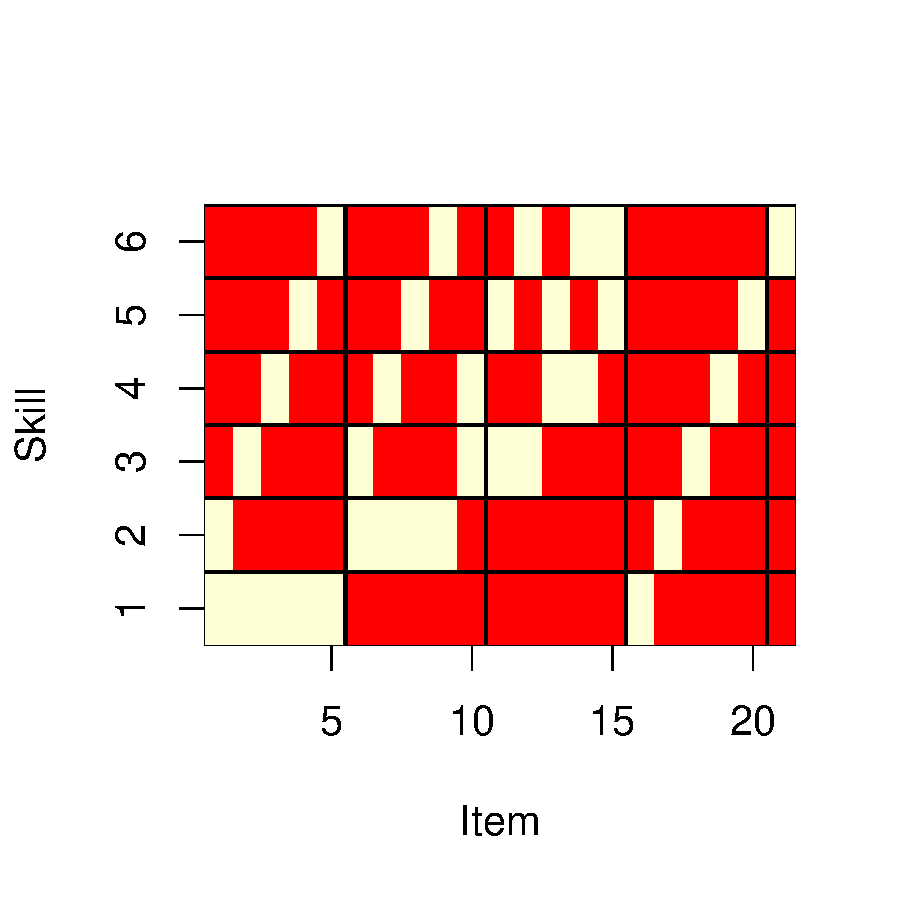
\includegraphics[scale =0.5] {ExpectedQ.pdf}\label{PerfectQ}
 }\quad
 \subfigure[Synthetic data of 100 students with 10\% slip and 20\% guess factor]{
   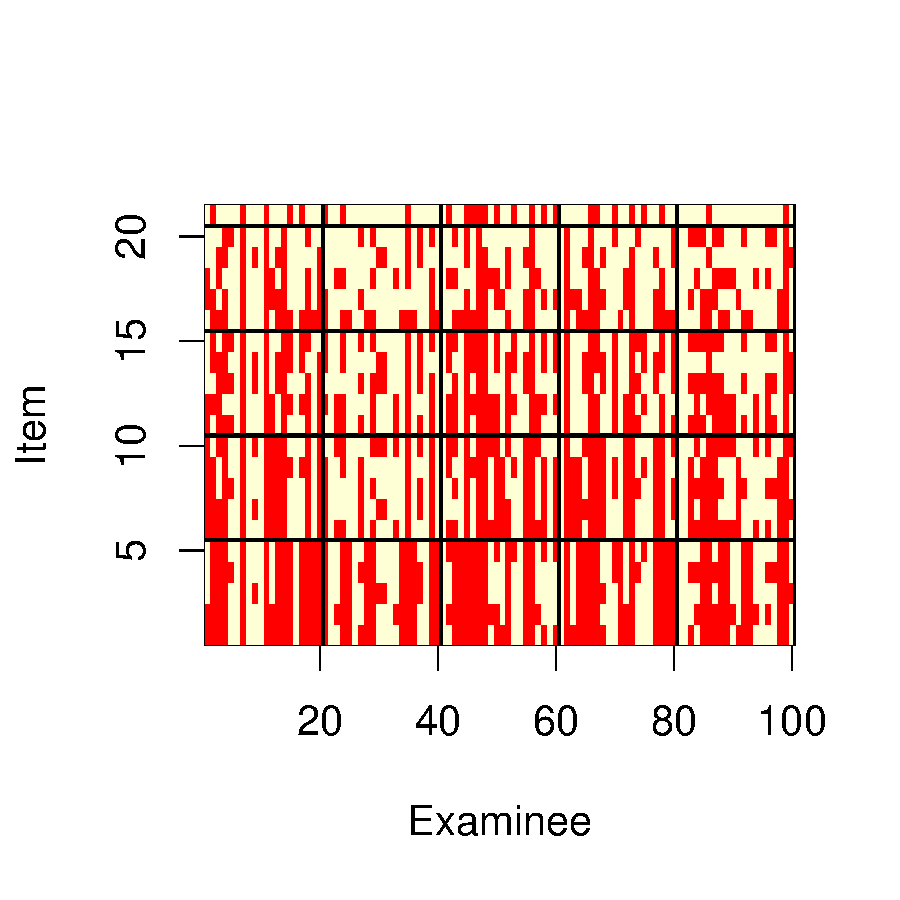
\includegraphics[scale =0.5] {ResultM.pdf}
 }
\caption{Q-matrix and an example of simulated data with this matrix.  pale cells represent 1's and red ones represent 0's.}
\label{figqmatrixandResutM}
\end{figure}

There are two ways to apply item variance in the simulated data and both of them are based on manipulating the values of the Q-matrix. Applying skills difficulty on skills would transfer the difficulty to items that have this skill. The other method is to consider the same weight for skills difficulty but controlling the item variance by assigning different number of skills to items. For example items with 1 skill would become easier to answer comparing to items with two or more skills where skills difficulty is the same for all skills. 

The second step is to create a student skills mastery matrix which maps $k$ skills to $m$ students. In terms of ability for examinees we assigned random values to skills for students but  student variance show up as the variance in number of skills across examinees. At the same time we can apply the overall success rate on the skill mastery matrix using a threshold to discrete the assigned values in skills mastery. 

Once the Q-matrix and Skills mastery matrix is created we can produce the test result matrix with equation~(\ref{eq:6}). The last step is to add slip and guess factors which are set as constant values across items.

A sample of the results matrix is given in figure~\ref{figqmatrixandResutM} where pale cells represent a value of 1 and red cells are 0. Examinee ability shows up as vertical patterns, whereas skills difficulty creates horizontal patterns. As expected, the mean success rate of the 2-skills items 1 to 15 is lower than the single skill items 16 to 21.

\section{Linear NMF Additive}

The process to create synthetic data based on additive type of Q-matrix is almost the same as Conjunctive one. The difference is on the interpretation of the Q-matrix that changes the step where the result matrix is producing.

For this case each cell in the Q-matrix should be normalized on the bases of items. Although each skill has a specific weight to success an item but in our experiment we consider equal weight for all skills of an item. For this purpose all the values assigning to each item in Q-matrix should be divided by the number of involved skills for that item.

\begin{figure}[h]
\begin{tabular}{c}
\subfigure[{Additive Q-matrix\label{figNMFAddQM}}]{\begin{footnotesize}
$\begin{array}{ccc}
 && \textrm{items}\\

\mathrm{\begin{sideways}skills\end{sideways}} & & \left[\begin{array}{cccccccccccccccccc}

0.5&0.00&0.25&0.33&0.33&0.33&0.00&0.5&0.5&0.5&0.0&0.0&0.0&1&0&0&0\\
0.0&0.33&0.25&0.33&0.33&0.00&0.33&0.5&0.0&0.0&0.5&0.5&0.0&0&1&0&0\\
0.0&0.33&0.25&0.33&0.00&0.33&0.33&0.0&0.5&0.0&0.5&0.0&0.5&0&0&1&0\\
0.5&0.33&0.25&0.00&0.33&0.33&0.33&0.0&0.0&0.5&0.0&0.5&0.5&0&0&0&1


\end{array}\right]
\end{array}$
\end{footnotesize}
}\\
\begin{tabular}{cc}
\subfigure[Raw Result matrix ]{
   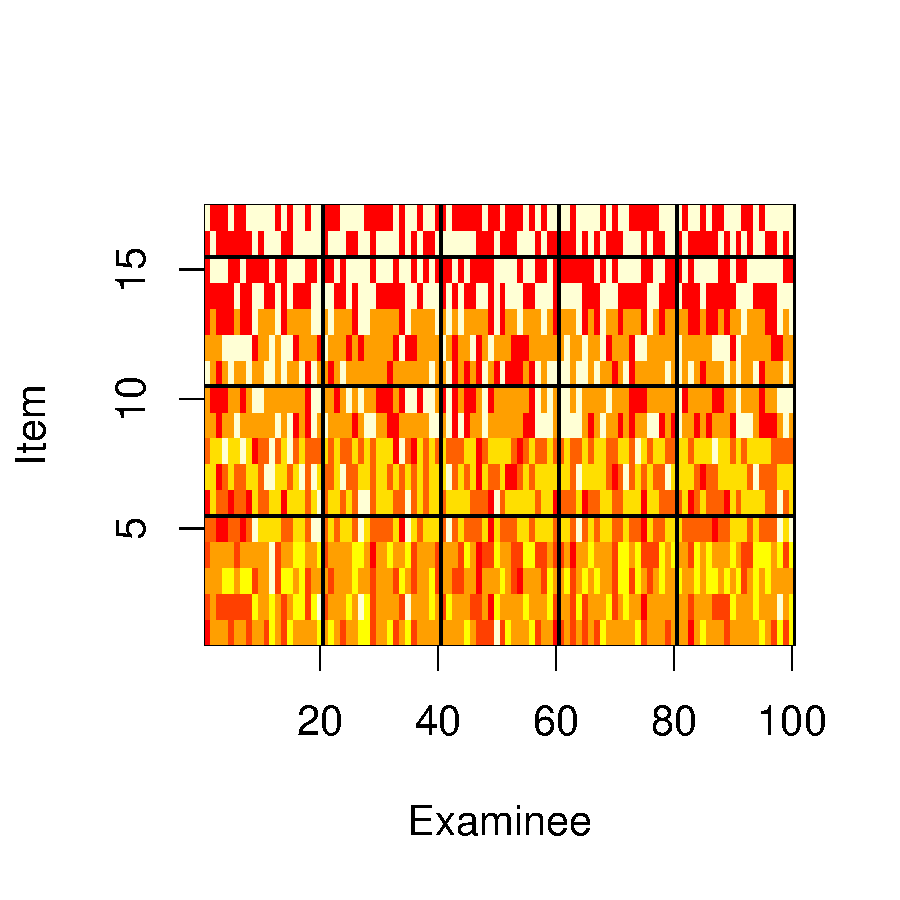
\includegraphics[scale =0.5] {NMFAddNonNoisy.pdf}\label{NMFAddNonNoisy}
 }\quad
&
\subfigure[Discretized result matrix with 20\% slip and 10\% guess factor]{
   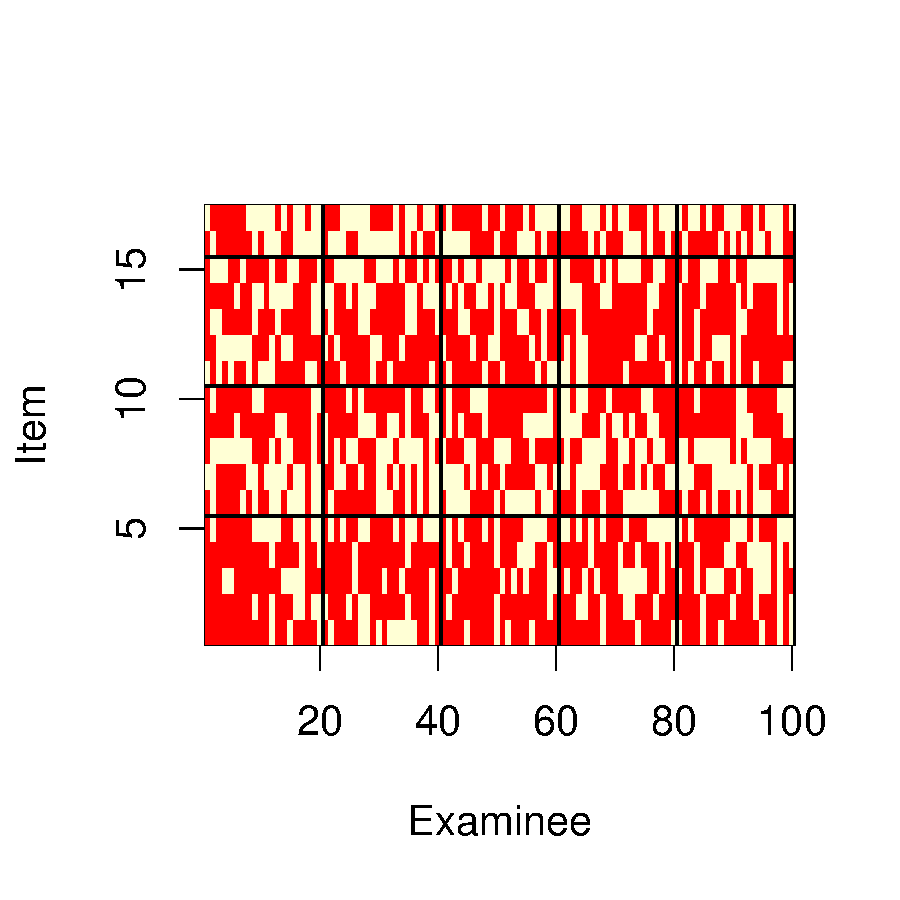
\includegraphics[scale =0.5] {NMFAddNoisy}\label{NMFAddNoisy}
 }\quad
\end{tabular}
\end{tabular}
\caption{Additive model of Q-matrix and Corresponding synthetic data}
\label{figNMFAddgen}
\end{figure}

Figure~\ref{figNMFAddQM} shows an additive type of Q-matrix and figure~\ref{NMFAddNoisy} is the result of cross product of this matrix to a students skills mastery matrix. Since the model is additive, there are some pale cells and the paler a cell is, the more chance a student has to success the question. In conjunctive model the result matrix is either $0$ or $1$. 

\section{DINA/DINO}
These models are also categorized as linear models that use a Q-matrix. The Q-matrix can be predefined for a better comparison or can be synthetic. For synthetic Q-matrix we use the same method as described before. At the same time we can control the number of skills and items in generation of a Q-matrix.

Equation~\ref{DinoEQ3} requires three parameters to predict a test outcome. In our experiment we create a sequence of values for guess and slip in the range of $0$ and $0.2\%$. Examinee's skills can be generated by a normal distribution which should match the number of skills presented in the Q-matrix. The difference between creation of skills mastery matrix in DINA/DINO and NMF is the way that skills are appearing for each student. In DINA/DINO there is a predefined set of possible combination of skills that can be used in skills mastery for each student. For example for 3 skills, this set can have maximum 8 combination. There is a distribution that is assigned to this set which defines the probability of appearance for each combination in the skills mastery matrix. 
\begin{equation}
 P(X_{ij} \!=\! 1 \; | \; \xi_{ij}) \,=\, (1-s_j)^{\xi_{ij}} g_j^{1-\xi_{ij}}
\label{DinoEQ3}
\end{equation}
We can apply total success rate during the creation of student's skills mastery matrix where students skills define the success rate of a dataset. Since these models are behaving based on a single value that represents student ability, we need to calculate an array of abilities for each item given a set of skills for an student. In DINO we use a disjunction between skills of an item and skills of a student to determine whether the student has the ability or not where for DINA a conjunction applies.


\Chapter{Experimental Results}\label{sec:SIGNATURE}

In this chapter we present a method of determining the model that is closest to the ground thruth by defining a space to characterize models based on their predictive performance.  A real data set is a point in that space, and synthetic data sets associated with each model are also individual points.  The model's synthetic data set that is the closest to the real data set is deemed the ground truth.  Details of this framework is described later. We first review the basic concepts and the models used in this study.


 % However, the approach would generalize to dynamic data as well.


\section{Model fit in a vector space framework}

The approach we propose to finding the model that best fits a data set is based on the assumption that the predictive performance of a given model will vary as a function of the data set's groud truth model, and that the relative performance between different data sets will be stable.

Let us explain this idea with the performance data in table~\ref{tab:vectorspace}, where the predictive accuracy of the 6~models reviewed in chapter~\ref{sec:RevLitt} is reported against 6~synthetic data sets generated with the same models.  A seventh ``model'' named \textit{expected} and seventh data set named \textit{random} are added for comparison purpose.  The details of the different models and of the methodology to assess model performance are described later.  For now, let us only focus on this table's data.

\newcolumntype{d}[1]{D{.}{.}{#1}} % not used

\begin{table}[ht]
\caption{Vector space of accuracy performances}\label{tab:vectorspace}
\centering
\begin{tabular}{lccccccc}
  \toprule
  \multicolumn{1}{c}{\multirow{2}{*}{\textbf{Model}}} & \multicolumn{7}{c}{\textbf{Synthetic data set}}\\
  \cline{2-8}
  & \multicolumn{1}{c}{{\textit{Random}}} & \multicolumn{1}{c}{{POKS}} & \multicolumn{1}{c}{{IRT}} & \multicolumn{1}{c}{{DINA}} & \multicolumn{1}{c}{{DINO}} & \multicolumn{1}{c}{{NMF.Conj}} & \multicolumn{1}{c}{{NMF.Comp}} \\ 
  \hline
  \textit{Expected} & \textbf{0.75} & 0.91 & 0.90 & 0.72 & 0.72 & 0.78 & 0.93 \\ 
  POKS & 0.75 & \textbf{0.94} & 0.94 & 0.81 & 0.81 & 0.90 & 0.94 \\ 
  IRT & 0.75 & 0.91 & \textbf{0.95} & 0.73 & 0.73 & 0.79 & 0.89 \\ 
  DINA & 0.75 & 0.77 & 0.81 & \textbf{1.00} & 0.65 & 0.98 & 0.89 \\ 
  DINO & 0.75 & 0.63 & 0.56 & 0.66 & \textbf{1.00} & 0.68 & 0.91 \\ 
  NMF.Conj & 0.75& 0.59 & 0.53 & 0.95 & 0.65 & \textbf{0.95} & 0.58 \\ 
  NMF.Comp & 0.75 & 0.76 & 0.79 & 0.59 & 0.93 & 0.70 & \textbf{0.98} \\ 
  \bottomrule
\end{tabular}
\end{table}


As we can expect, the diagonal (in bold face) always displays the best performance since it corresponds to the alignment of the model and the ground truth behind the data.  This confirms the intuition behind the usual strategy of assuming the best performer is the model behind the ground truth.  However, this is not always the case as we will see later.

The principle of the proposed approach is to use the whole column of performance as a vector to determine the closest model to the ground truth.  In that respect, if columns are considered as vectors in the space of dimensions created by model performances, we can use a similarity measure to determine the closest ground truth (or a distance measure if we were to consider the columns as a point in space).

The advantage of this approach is that it does not rely on a single performance value to determine the goodness of fit, but instead on a set of performances over different models.  The hypothesis is that this set of performances provides a more reliable measure of the goodness of fit of a set of models.  In turns, we assume that this measure is more likely to indicate which model will perform better in general, as opposed to which models performs the best in the case of the single data set at hand.  

The approach can be considered as a means to avoid a kind of local minimum, considering the best performer as a good indicator of the ground truth, but not a perfect one. Indeed, table~\ref{tab:vectorspace} suggests that aligning the model with the ground truth does yield the best performance, but we will show examples later that there are exeptions and that the proposed approach is better able to avoid these exceptions that would lead to a wrong conclusion if we were to rely on the best performer approach.




\section{Methodology}

In a first experiment, we focus on showing the performance of all models over synthetic and real data sets.  It provides an overview of the relative performance of each model across the different synthetic data sets and across real data as well. 

In a second experiment, we move focus to the central problem of this paper: classifying data sets in the performance vector space.  To validate the approach, we need to rely solely on synthetic data for which we know the underlying ground truth model.  A matrix such as the one in figure~\ref{AssessMethods} is created with data sets generated from the different models, and each model performance is measured through a cross validation process.  This matrix allows us to classify a data set of unknown ground truth according to a nearest neighbour approach.  

%%%%%%%%%%%%%%%%%%%%%%%%%%%%%%%%%%%%%%%%%%%%%%%%%%%%%%%%%%%%%%%%%%%%%%%%%%%%%
\section{Experiment 1: Performance comparison}

The performance of each model is assessed on the basis of 10-folds cross-validation.  The training set is used to estimate model parameters that are later used in for the test set. For each test set, a model is fed with a set of item outcomes of a student, called the observed set, and the remaining items are the predicted, or inferred ones. The breakdown of the data for cross-validation is illustrated in figure~\ref{figMethod}. We fixed the number of observed items for each run on each data set. The minimum number of observed items is 9 and the maximum number is one item less than total number of items. 

\begin{figure}
\centering
{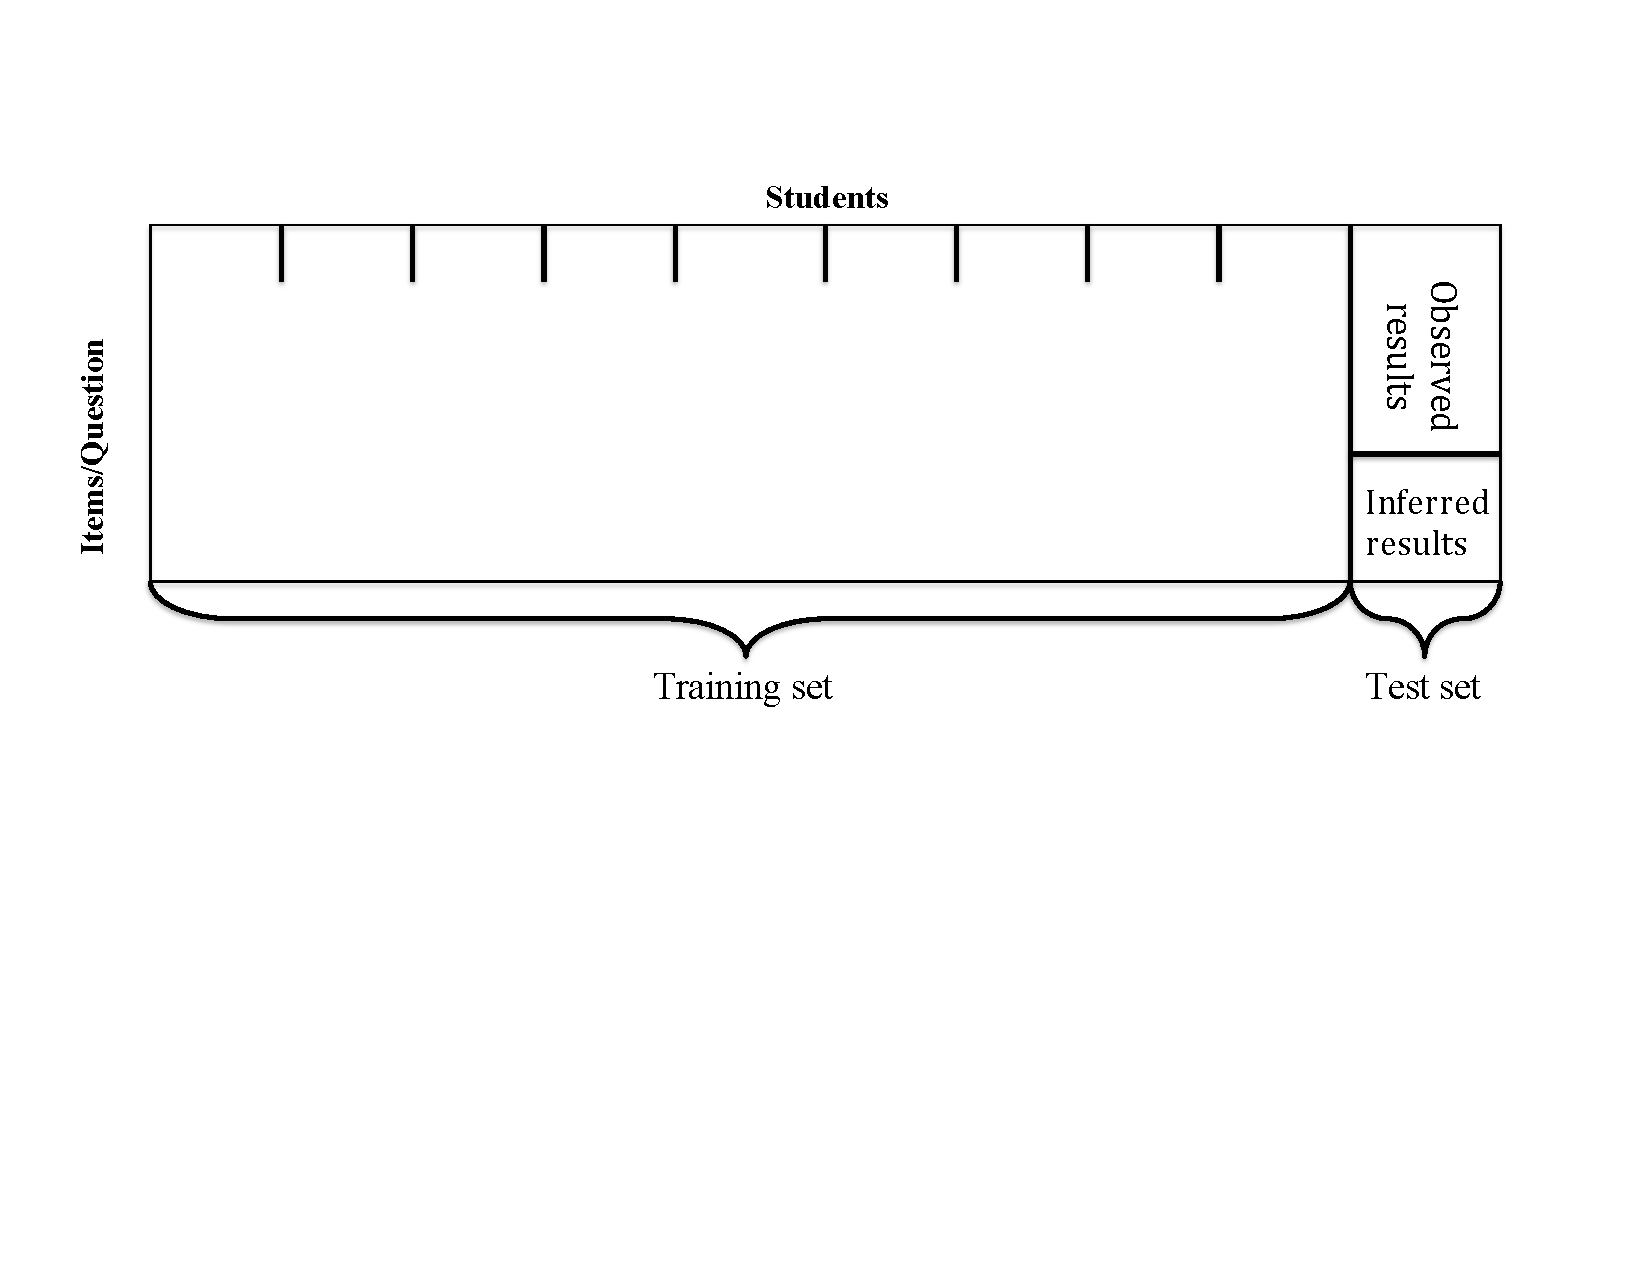
\includegraphics[trim=2cm 9cm 2.4cm 2.4cm,clip=true,width=.6\textwidth]{Images/Methodology.pdf}}
\caption{Data breakdown of cross validation process}
\label{figMethod}
\end{figure}

For each dataset there exists a training set that contains 9 folds and a test set that which represents a single fold. A list of required parameters are presented in table~\ref{fig:param}. Samples are assigned randomly to each fold and this setting is the same across all predictive models for each run. Since all items are presented in the training set, then we can estimate the parameters that are related to items. 

\begin{table}
  \centering

  \begin{tabular}{>{\raggedright}p{.02\textwidth}>{\raggedright}p{.3\textwidth}>{\raggedright}p{.15\textwidth}>{\raggedright}p{.4\textwidth}}
    \toprule
    & \multicolumn{1}{c}{\textbf{Parameter}} & \multicolumn{1}{c}{\textbf{Typical values}} & \multicolumn{1}{c}{\textbf{Models affected}} \tabularnewline
    \toprule
    \multicolumn{3}{l}{\textbf{Data specific parameters}}\tabularnewline
    \cline{2-4}
    & Number of skills & \numrange{3}{9} & Multiple skills models:\newline DINA, DINO, NMF Conj./Add. \tabularnewline
    \cline{2-4}
    & Number of items & \numrange{10}{50} &   \tabularnewline
    \cline{2-3}
    & Number of students & \numrange{100}{1500} & \tabularnewline
    \cline{2-3}
    & Test success rate & \numrange{0.25}{0.85}   &\tabularnewline
    \cline{2-3}
    & Student score variance & \numrange{0.03}{0.20} & \tabularnewline
    \cline{2-3}
    & Item score variance & \numrange{0.03}{0.20} & \multirow{-5}{*}{All models} \tabularnewline
    \cline{2-4}
    & Item discrimination & \numrange{0.5}{3} & \tabularnewline
    \cline{2-3}
    & Item difficulty & \numrange{-3}{3} & \tabularnewline
    \cline{2-3}
    & Student ability & \numrange{-4}{4} & \multirow{-3}{*}{IRT} \tabularnewline
    \hline
    \multicolumn{3}{l}{\textbf{Simulation parameters}}\tabularnewline
    \cline{2-4}
    & Number of observed items &  9 to Number of items -1 & \tabularnewline
    \cline{2-3}
    & Training set size & 90\% of $[100-1500]$ &  \multirow{-2}{*}{All models}\tabularnewline
    \hline
    \multicolumn{3}{l}{\textbf{Model specific parameters}}\tabularnewline
    \cline{2-4}
    & Guess and slip & $[0.0-0.2]$ & DINO and DINA\tabularnewline
    \cline{2-4}
    & Binomial and interaction tests & $\alpha_1=0.85\newline \alpha_2=0.10$ & POKS\tabularnewline
    \bottomrule
  \end{tabular}
  \caption{Parameters of the simulation framework}
  \label{fig:param}
\end{table}


\newcommand{\tabitem}{~~\llap{\textbullet}~~}
\newcommand\VRule[1][\arrayrulewidth]{\vrule width #1}



\begin{table}
  \centering

\begin{tabular}{c|c|l!{\VRule[1.5pt]}l|l!{\VRule[1.5pt]}l|}
\multicolumn{3}{c}{}&\multicolumn{3}{c}{Parameters estimated from}\tabularnewline
\cline{4-6}
\multicolumn{3}{c!{\VRule[1.5pt]}}{Skills Model}&\multicolumn{2}{c!{\VRule[1.5pt]}}{Training set}&Observed items\tabularnewline
\cmidrule[1.5pt]{2-6}
&&NMF Conj. & & &  \tabularnewline
\cline{3-3}
&&NMF Add.&&& \tabularnewline
\cline{3-4}
&&DINA& \tabitem Slip & &\tabularnewline
\cline{3-3} 
&\multirow{-4}{*}{\begin{sideways} \scriptsize Multiple\end{sideways}}&DINO& \tabitem Guess&\multirow{-4}{*}{ \tabitem  Q-matrix }&\multirow{-4}{*}{  \parbox[t]{3cm}{ \tabitem Students skills  \\ mastery matrix}} \tabularnewline
\cmidrule[1.5pt]{2-6}
&&&\multicolumn{2}{l!{\VRule[1.5pt]}}{\tabitem Item difficulty  } &  \tabularnewline
&&\multirow{-2}{*}{ IRT}&\multicolumn{2}{l!{\VRule[1.5pt]}}{\tabitem Item discrimination}  &\multirow{-2}{*}{\tabitem Student Ability} \tabularnewline
\cline{3-6}
&\multirow{-3}{*}{\begin{sideways} \scriptsize Single \end{sideways}}&Expected&\multicolumn{2}{l!{\VRule[1.5pt]}}{\tabitem Item Odds}  &\tabitem Student Odds \tabularnewline
\cmidrule[1.5pt]{2-6}
&&&\multicolumn{2}{l!{\VRule[1.5pt]}}{\tabitem Initial Odds } & \tabularnewline
&&&\multicolumn{2}{l!{\VRule[1.5pt]}}{ \tabitem Odds ratio } & \tabularnewline
\multirow{-9}{*}{\begin{sideways} \scriptsize Contributed skills \end{sideways}}&\multirow{-3}{*}{\begin{sideways} \scriptsize Zero\end{sideways}}&\multirow{-3}{*}{ POKS }&\multicolumn{2}{l!{\VRule[1.5pt]}}{\tabitem PO structure}&\multirow{-3}{*}{ }\tabularnewline
\cmidrule[1.5pt]{2-6}
\end{tabular}
  \caption{Parameters of the predictive performance framework}
  \label{fig:param-Predictive-Performance}
\end{table}


For other parameters that are related to students we need to divide the test set into an observed and inferred set. From the observed set we can get to the parameters that are related to students. A list of required parameters for assessing the model performance in table~\ref{fig:param-Predictive-Performance}.

Once all the required parameters are presented we can make a prediction for the inferred cells of the result matrix. Note that the selected observed and inferred items are the same across all the models for each run to make a better comparison for their prediction. A probability of mastery is obtained and rounded, resulting in a 0/1 error loss function.  We report the mean accuracy as the performance measure.  The R package \texttt{ltm} is used for parameter and skills estimation for IRT model and the R package \texttt{CDM} and \texttt{NMF} for Deterministic noisy and NMF models. A comparison between the predicted results and the real values can result in a performance accuracy. 


%%%%%%%%%%%%%%%%%%%%%%%%%%%%%%%%%%%%%%%%%%%%%%%%%%%%%%%%%%%%%%%%%%%%%%%%%%%%%
\subsection{Data sets}

The performance of the models is assessed over a total of 14~data sets, 7~of which are synthetic, and 7~are real data.  They are listed in table~\ref{tabl1}, along with the number of skills of their Q-matrix, their number of items, the number of the student respondents, and the average score.  Table~\ref{tabl1} also reports the Q-matrix used.  As can be seen, some synthetic data sets share their Q-matrix with real data sets.  This sharing allows greater similarity between the synthetic data and a real data counterpart that shares a Q-matrix.  Other parameters used to create the synthetic data sets were also obtained from real data sets with the same intent of allowing better comparison.  

Of the 7~real data sets, only three are independent.  The other~4 are variations of a well known data set in fraction algebra from Tatsuoka's work \citep{tatsuoka1984analysis}.  They consists in subsets of questions and variations of the Q-matrix.  These variants allows us to explore the effect of different models (Q-matrices) over the same data source.

The Vomlel data was obtained from \citep{vomlel:2004} and is also on the topic of fraction algebra.  The Q-matrix for this data is derived from the Bayesian Network defined over the 20~item test by experts.

The ECPE data (Examination for the Certificate of Proficiency in English) is an English as a foreign language examination. It is recognized in several countries as a test of advanced proficiency in English and used by a number of universities.

These real data sets were obtained from different sources and are freely available from the CDM \citep{Robitzsch2012} and NPCD ({\url{http://cran.r-project.org/web/packages/NPCD/}}) R packages. The Q-matrices of the real data sets were made by experts.


\newcounter{i}\setcounter{i}{1}
\newlength{\mdnum}
\setlength{\mdnum}{\widthof{10}}
\newlength{\mdnumtwo}
\setlength{\mdnumtwo}{\widthof{$\mathbf{Q}_{01}$}}
\newcommand{\mdcount}[2]{\parbox{#1}{\hfill\arabic{i}}.\ #2\addtocounter{i}{1}}
\begin{table}
\centering
\footnotesize
%\begin{tabular}{|l|c|c|r|r|l|}
\begin{tabular}{|l|c|c|r|r|l|}
\hline

%\rowcolor{\color[rgb]{.8,.8,.8}}
\multirow{2}{*}{Data set} & \multicolumn{3}{c|}{Number of} & {\parbox{6ex}{\center Mean\\Score}} & \multirow{2}{*}{Q-matrix}\tabularnewline
\cline{2-4} 
%\rowcolor{\color[rgb]{.8,.8,.8}}
 & Skills & Items & Students &  & \tabularnewline
\hline
\hline
%\rowcolor{\color[rgb]{.9,.9,.9}}
\multicolumn{6}{|c|}{\textit{Synthetic}}\\
\hline
\hline
\mdcount{\mdnum}{Random} & 7 & 30 & 700 &0.75& $\mathbf{Q}_{01}$\tabularnewline
\hline
\mdcount{\mdnum}{POKS} & 7 & 20 & 500 &0.50 & $\mathbf{Q}_{02}$\tabularnewline
\hline
\mdcount{\mdnum}{IRT-2PL} & 5 & 20 & 600 &0.50& $\mathbf{Q}_{03}$\tabularnewline
\hline
\mdcount{\mdnum}{DINA} & 7 & 28 & 500 &0.31& $\mathbf{Q}_5$\tabularnewline
\hline
\mdcount{\mdnum}{DINO} & 7 & 28 & 500 &0.69& $\mathbf{Q}_6$\tabularnewline
\hline
\multicolumn{6}{|l|}{Linear (Matrix factorization)}\\
\hline
\mdcount{\mdnum}{~~~Conj.} & 8 & 20 & 500 &0.24& $\mathbf{Q}_1$\tabularnewline
\hline
\mdcount{\mdnum}{~~~Comp.} & 8 & 20 & 500 &0.57& $\mathbf{Q}_1$ \tabularnewline
\hline
\hline
%\rowcolor{\color[rgb]{.9,.9,.9}}
\multicolumn{6}{|c|}{\textit{Real}}\\
\hline
\hline
\mdcount{\mdnum}{Fraction} & 8 & 20 & 536 &0.53& $\mathbf{Q}_1$\tabularnewline
\hline
\mdcount{\mdnum}{Vomlel} & 6 & 20 & 149 &0.61& $\mathbf{Q}_4$\tabularnewline
\hline
\mdcount{\mdnum}{ECPE} & 3 & 28 & 2922 &0.71& $\mathbf{Q}_3$\tabularnewline
\hline
\multicolumn{6}{|l|}{Fraction subsets and variants of $\mathbf{Q}_{1}$}\\
\hline
\mdcount{\mdnum}{~~~1} & 5 & 15 & 536 &0.53& $\mathbf{Q}_{10}$\tabularnewline
\hline
\mdcount{\mdnum}{~~~2/1} & 3 & 11 & 536 &0.51& $\mathbf{Q}_{11}$\tabularnewline
\hline
\mdcount{\mdnum}{~~~2/2} & 5 & 11 & 536 &0.51& $\mathbf{Q}_{12}$\tabularnewline
\hline
\mdcount{\mdnum}{~~~2/3} & 3 & 11 & 536 &0.51& $\mathbf{Q}_{13}$\tabularnewline
\hline
\hline
\end{tabular}
\caption{Datasets}
\label{tabl1}
\end{table}


The synthetic data sets are generated from each skills assessment model, with an effort to fit the parameters as closely as possible to a real data counterpart that shares the same Q-matrix.  

For POKS, the structure was obtained from the Fraction data set and the conditional probabilities were generated stochastically, but in accordance with the semantic constraints of these structures and to obtain an average success rate of 0.5.

For IRT, the student ability distributions was obtained from the Fraction data set, and the item difficulty was set to reasonable values: averaging to 1 and following a Poisson distribution that kept most values between 0.5 and 2 (done by generating random numbers from a Poisson distribution with lambda parameter set to 10 and dividing by 10). 

The matrix factorization synthetic data sets of DINO and DINA were generated by taking a Q-matrix of 7~skills that contains all possible combinations of 1 and 2~skills, which gives a total of 28~combinations and therefore the same number of items.  Random binary skills matrix (which corresponds to matrix~$\mathbf{S}$ in equation~(\ref{eq:1}) were generated and the same process was used for both the DINO and DINA data sets.  Item outcome is then generated according to equation~(\ref{DinoEQ}) with a slip and guess factor of 0.1.

A similar process was followed to generate the Q-matrices and the skills matrices~$\mathbf{S}$ of the linear matrix factorization data sets, except that item outcome follows equation~(\ref{eq:1}) and is discretized.

%% MD: Investigate differences in correlations between items across real vs. synthetic data

Note that the first 4~models do not rely on any Q-matrix for the data generation process, but the DINO/DINA and matrix factorization assessment models still require one.  To define these Q-matrices (denoted~$\mathbf{Q}_{0x}$ in table~\ref{tabl1}, a wrapper method was used to first determine the number of skills according to \citep{Beheshti2012Numbers}, then a Q-matrix was derived with the deterministic ALS algorithm as described in section~\ref{ALS-Def}, starting with an initial random Q-matrix.
%% MD: Behzad, is this right?


%%%%%%%%%%%%%%%%%%%%%%%%%%%%%%%%%%%%%%%%%%%%%%%%%%%%%%%%%%%%%%%%%%%%%%%%%%%%%
\subsection{Predictive performance results} \label{secSyn}

This section shows the result of predictive performance of the seven models over the 14~datasets described in table~\ref{tabl1}. 

\begin{figure}
\centering
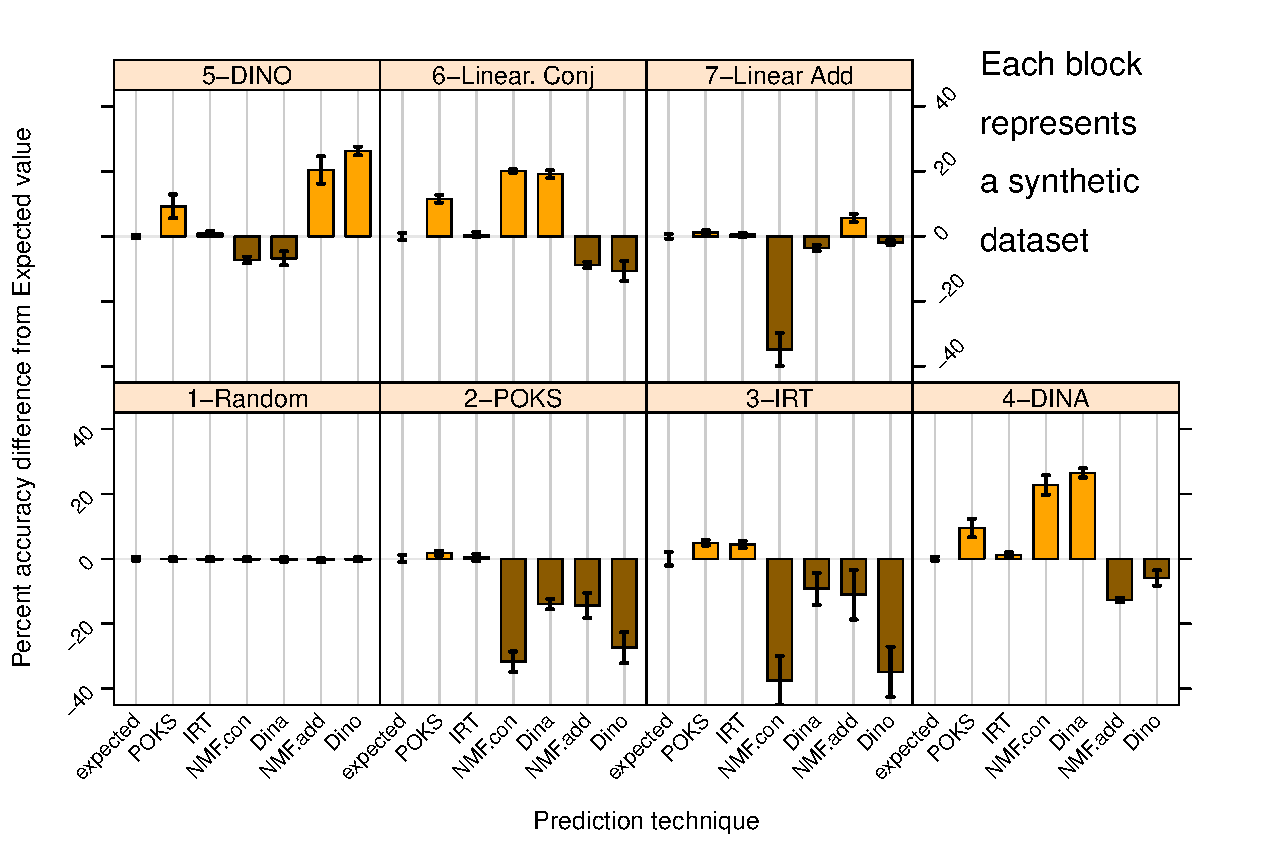
\includegraphics[clip=true,width=.9\textwidth]{Syn.pdf}
\caption{Item outcome prediction accuracy results of {\textbf{synthetic data sets}}}
\label{fig1}

{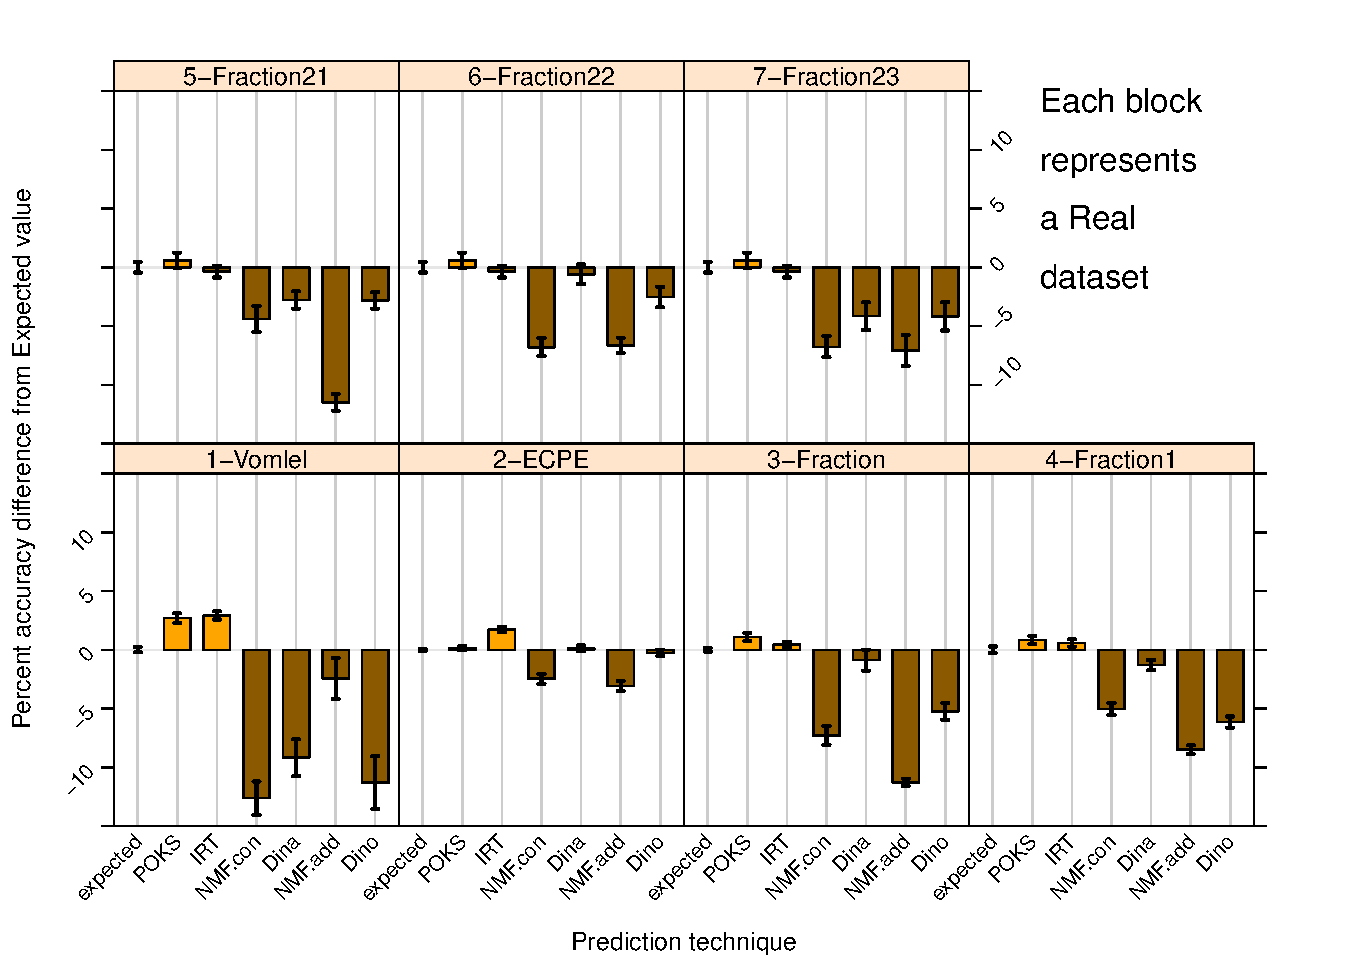
\includegraphics[clip=true,width=.9\textwidth]{Real.pdf}}
\caption{Item outcome prediction accuracy results of {\textbf{real data sets}}}
\label{fig2}
\end{figure}
%% We should eventually change the scale to logit so that the differences are more pronounced at the extremes
%% (or maybe just rescale from min-max for each data set)

Figures~\ref{fig1} and~\ref{fig2} show the performance of each model over the synthetic and real data sets.  The performance is the difference in accuracy of each model from the expected value, which serves as a baseline. Note that the y-scale of the synthetic data is double the one of the real data sets, and therefore the differences in performance for the synthetic datasets are much wider.  An error bar of 1~standard deviation is reported, computed over 10 simulation runs that each run considers four different number of observation that varies between 9 to an item less than maximum number of items, provides an idea of the variability of the results. A dataset of random data is also reported for a~$0.75$ average success rate.

As expected, when the generative model behind the synthetic data set is the same as the skills assessment technique, the corresponding technique's performance is the best, or close to the best.  And this performance is also always above the expected value performance, except for the random data set where not model can do any different than the expected value, which is what we would expect.

For the synthetic data sets, three models reach performances that are much higher than the baseline, in the range of $20-30$\% (DINO, Linear Conjunctive, and DINA), whereas for the three other models the gain is closer to 5\% (Linear additive, POKS, and IRT).

An important observation is that the pattern of relative differences of performances across techniques varies considerably and is unique to each data set: no two data sets have the same pattern of relative performance across models.  The capacity of recognizing a data set's true model relies on this uniqueness characteristic.

For the real data sets, the relative performance among the techniques shows smaller discrepancies and is closer to the baseline. Although the best performers are still significantly better than the expected values for the majority of the data sets, it is surprising to see that a majority of models do worst than the baseline for a majority of data sets. 

The results from the subsets of the Fraction data show that the pattern of the Fraction performance data set repeats over Fraction-1, Fraction-2/1 and Fraction-2/2, in spite of the different number of skills and different subsets of questions.  However, it differs substantially from Fraction-2/3 for the NMF conjunctive performance which reaches that of the NMF additive one and also DINA reaches DINO. This is readily explained explained by the fact that the Q-matrix of this data set has the property of assigning a single skill to each item, in which case the two matrix factorization techniques become equivalent.  But aside from the Fraction-2/3 case, this similarity among Fraction data set and its derivative suggests that in spite of the model differences (different Q-matrices and item subsets), the performance ``signature'' remains constant across these data sets.

Finally, we note that none of the real data sets show the large the discrepancies found in the synthetic data sets models. One exception is the linear additive synthetic data set which displays smaller variance across models and which ``signature'' resembles the Vomlel data, although the performance difference with the majority class is substantially higher for the synthetic data than the Vomlel data, suggesting that the real data is yet not a perfect fit to this model.
%% MD: we need to test this with the same Q-matrices.

%\begin{figure}
%  \centering

%    \includegraphics[scale=0.6]{Images/numberofObs.pdf}
%     \caption{Synthetic datasets with different number of observation}
%\label{figSampleSize}
%\end{figure}

\section{Experiment 2: Sensitivity of the Model performance over data generation parameters}
\label{Sensitive}

In this experiment we want to examine the effect of data generation parameters on the stability of the model performance vector in the performance space. In this section we run the same experiment but with different parameters such as average success rate, sample size, number of latent skills, number of items, student and item score variance. These factors can can answer the question whether the patterns hold across different conditions. Table~\ref{fig:param} shows different conditions of the parameters.

Just like the previous experiment, we assessed these results on the basis of 10-folds cross-validation. The same as before, we fixed the number of ``observed items'' for each run on each data set that varies between 9 to one item less than total number of items.

We generated the synthetic datasets with different sample size which varies from 100 students upto 1500 students. Figure~\ref{figSampleSize} shows the result of this change. Running all these techniques on the synthetic datasets did not change any pattern except for IRT generated dataset that slightly changed the pattern for small sample size. On the other cases the one with the highest predictive performance was the same as model behind the generated data. Also changing the sample size downto less than 100 students will change the pattern as well; because the training set of the model could not be Learned properly.


\begin{figure}
  \centering

    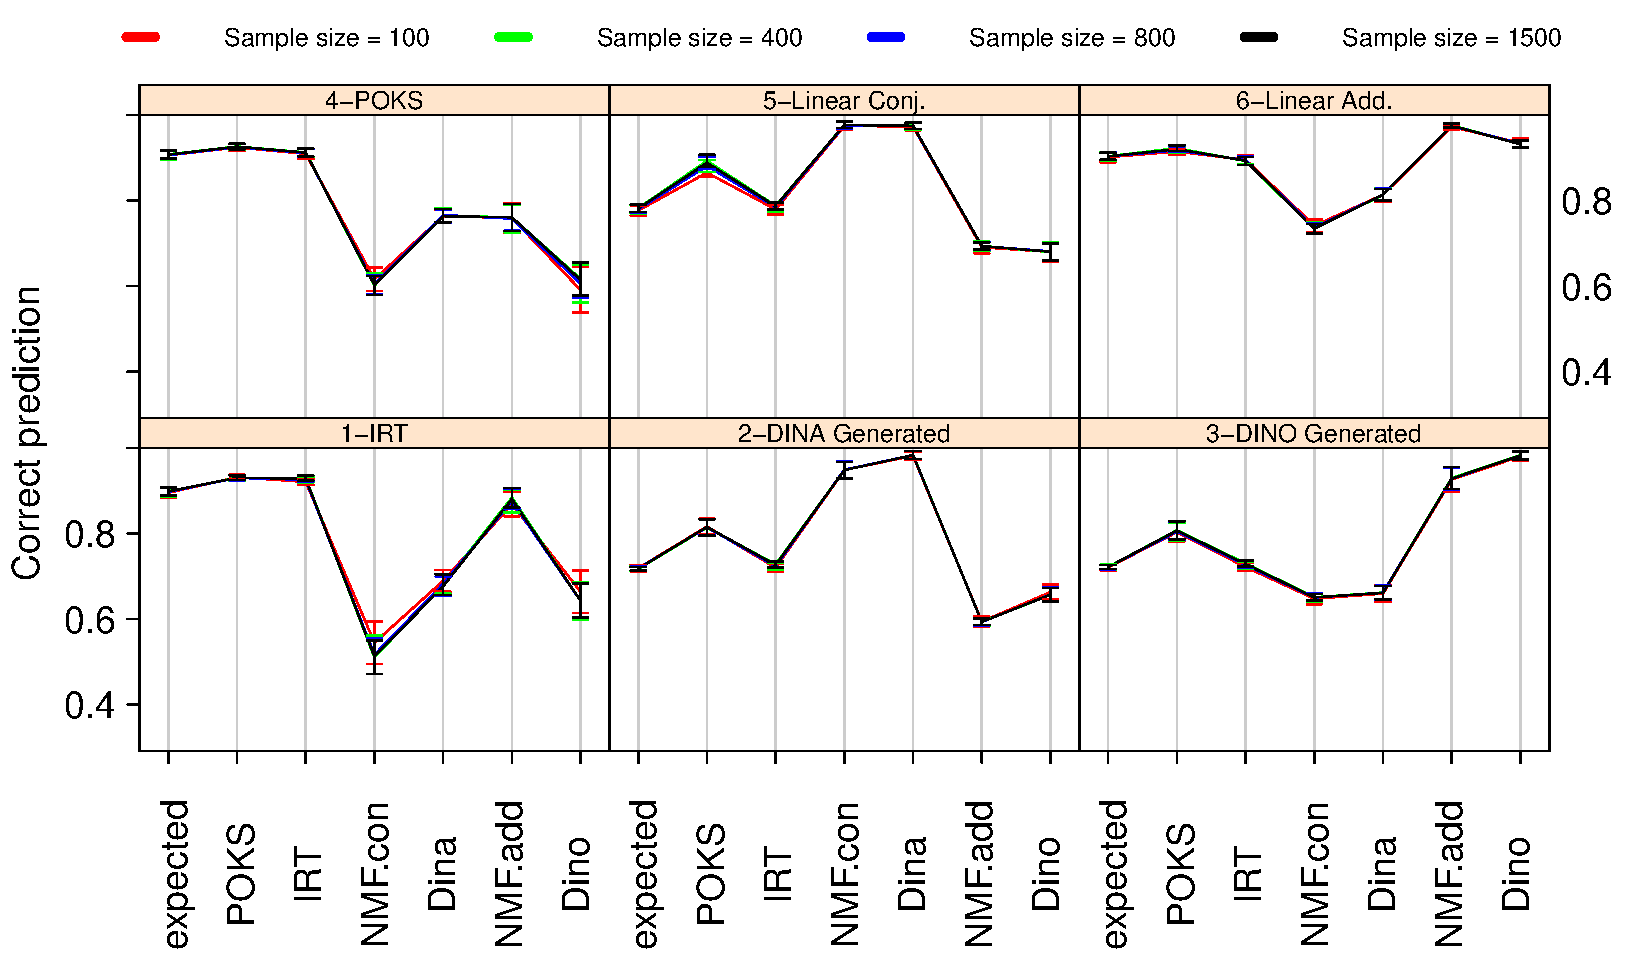
\includegraphics[scale=0.58]{SampleSize.pdf}
     \caption{Variation of \textbf{Sample Size} Over synthetic data sets}
\label{figSampleSize}
\end{figure}

The other parameter is the number of Items in generation of the synthetic dataset. This time we fixed all the other parameter but the Items size which varies between 10 to 50 items. Figure~\ref{figNumberofItems} shows how signature has been changed for different models. The results on the synthetic datasets shows that in some cases the pattern stays the same but it shifts down on the chart once we decrease the number of items. Still we can see that the highest performance is the same model behind the generated dataset. This highlights the role of this variable in predicting the signature and also means that the highest performance should not necessary be close to 100\%.

\begin{figure}
  \centering
    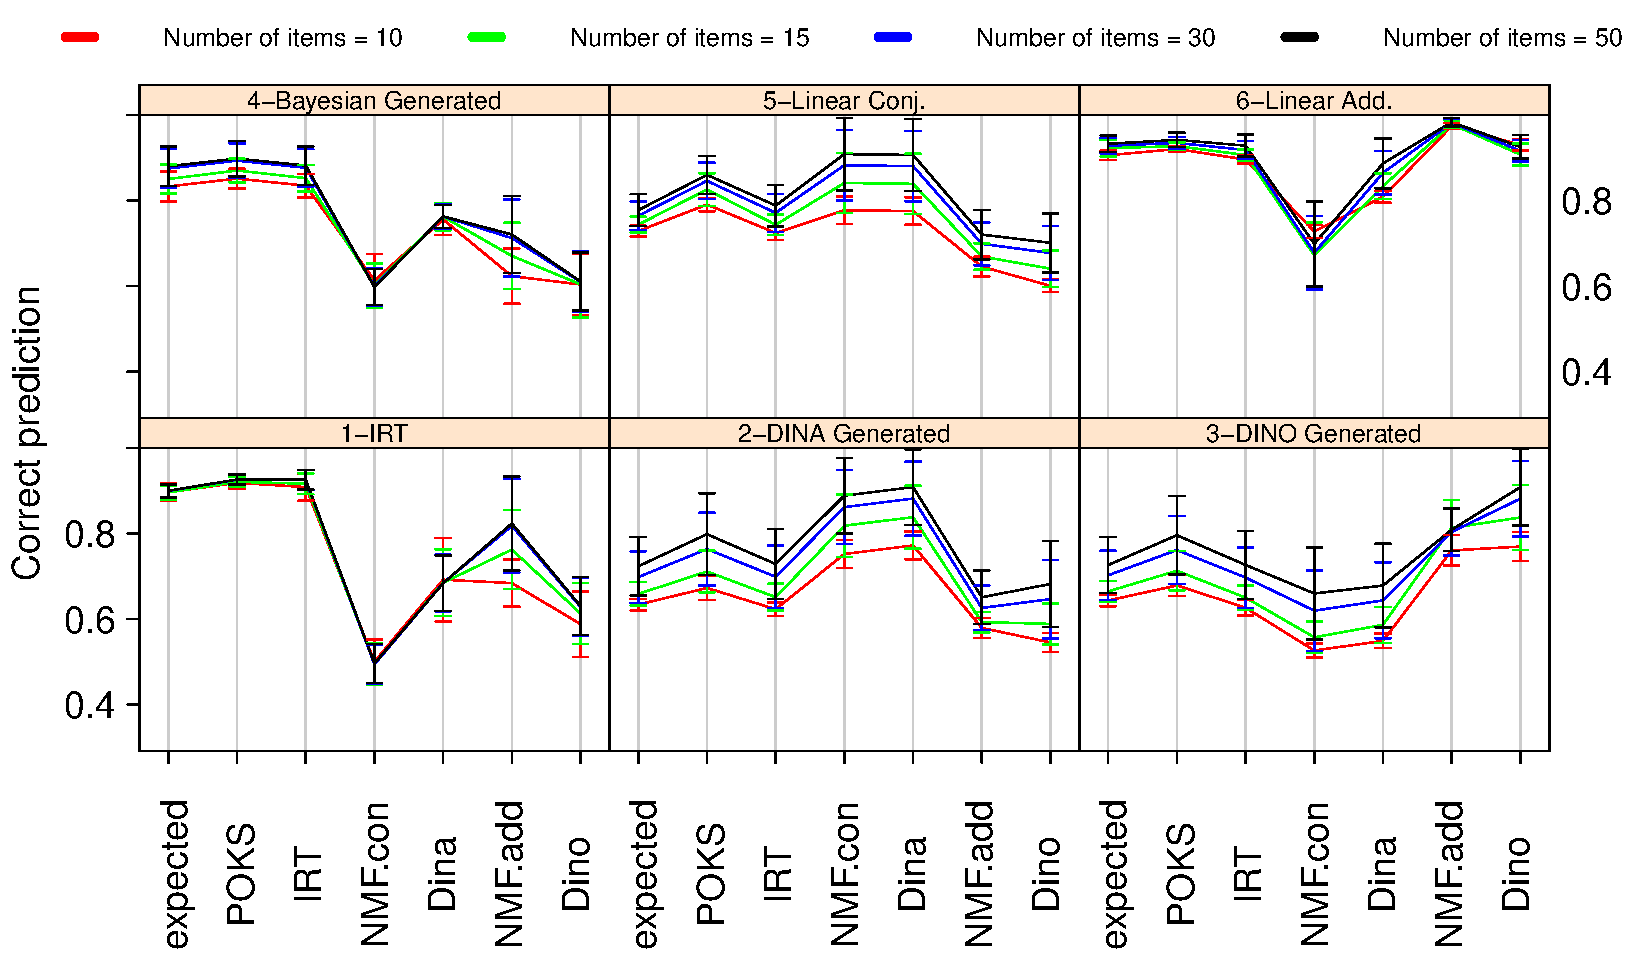
\includegraphics[scale=0.58]{numberofitems.pdf}
\caption{Variation of \textbf{Number of items} Over synthetic data sets}
\label{figNumberofItems}
\end{figure}

\begin{figure}
  \centering
    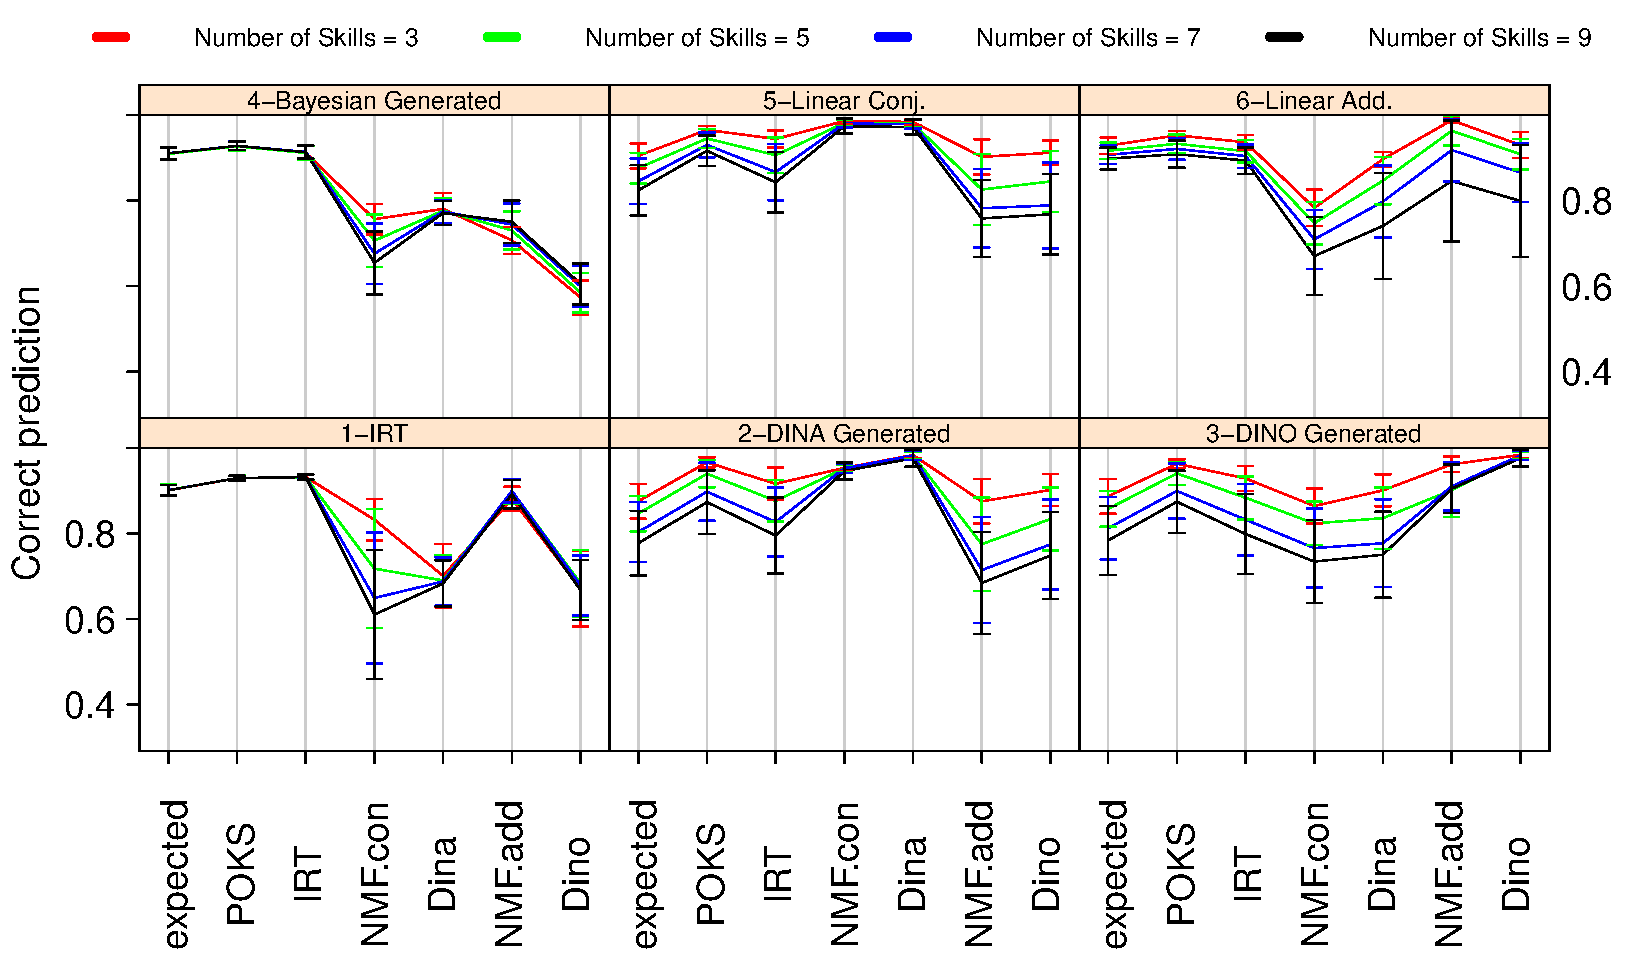
\includegraphics[scale=0.58]{numberofskills.pdf}
\caption{Variation of \textbf{Number of skills} Over synthetic data sets}
\label{figSkills}
\end{figure}

Next variable is number of skills in generation of dataset and estimation of the signature. Same as before we fixed all the other variables to generate the dataset but the number of skills behind the generation of the synthetic dataset which has been in the range of 3 to 9 skills in total. Figure~\ref{figSkills} shows the result of this experiment. For IRT and POKS generated dataset it does not make sense to have number of skills because IRT is a single skill model and there are no explicit latent skills. In order to find the predictive performance of linear methods for bayesian or IRT generated datasets we need to have a fixed number of skills as a part of prediction and that is how we run the experiment with different number of latent skills. The signature pattern did not change substantially for these datasets. Only for linear based techniques we can find a slight change in the pattern. For linear models the pattern still stays the same but for NMF additive when the number of skills increases the ground truth is not the highest performance in the signature. Increasing the number of skills while the number of item is constant can resemble the single skill modeling such as IRT and POKS. 

Figure~\ref{figitemVar} shows the same experiment across datasets with different item variance. The item variance was reflected as the item difficulty for IRT and initial odds for POKS. The value for item variance shows the standard divination of the normal distribution of the items. Clearly the pattern stays the same for different values except for few minor changes. Although the the set of performance values shifts across correct prediction axis but the pattern stays the same.

Finally, we did a last experiment on datasets with different success rates. For synthetic data, the success rate starts from 0.25\% up to 0.85\%. The pattern is scaled for some linear methods on IRT and bayesian generated data and it doesn't change the performance of IRT and POKS themselves. For datasets with linear structure the signature was shifted downward on linear methods predictive performance side as we decrease the success rate for data generation.


\begin{figure}
  \centering
    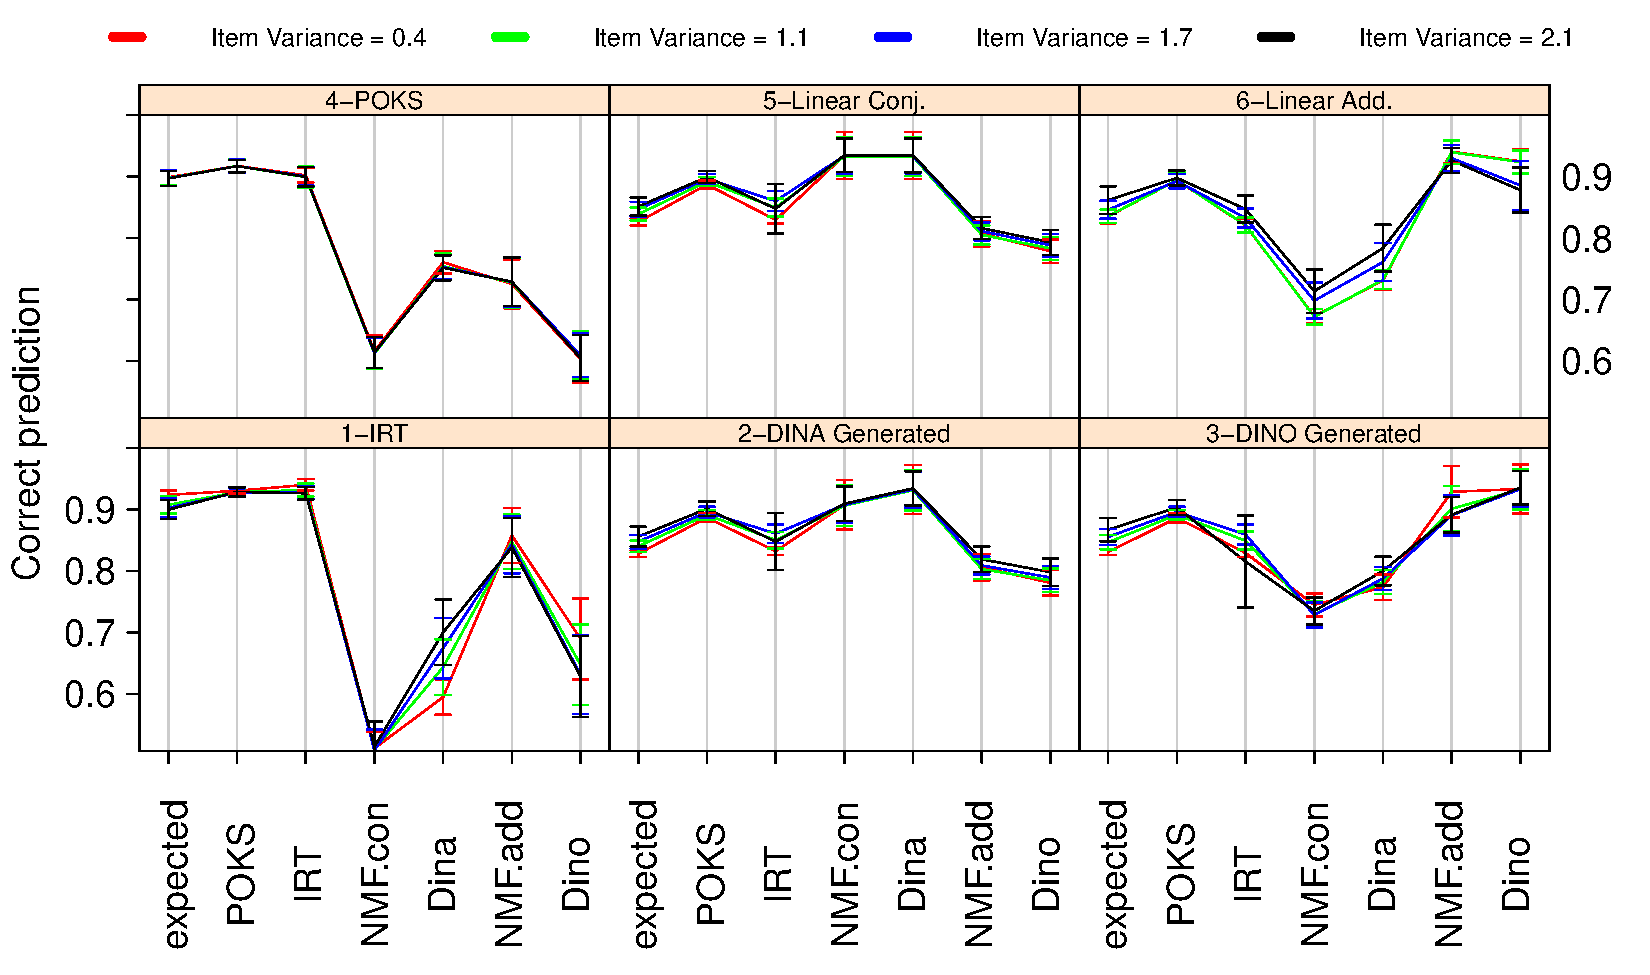
\includegraphics[scale=0.58]{ItemVariance.pdf}
\caption{Variation of \textbf{Item Variance} Over synthetic data sets}
\label{figitemVar}
\end{figure}

\begin{figure}
  \centering
    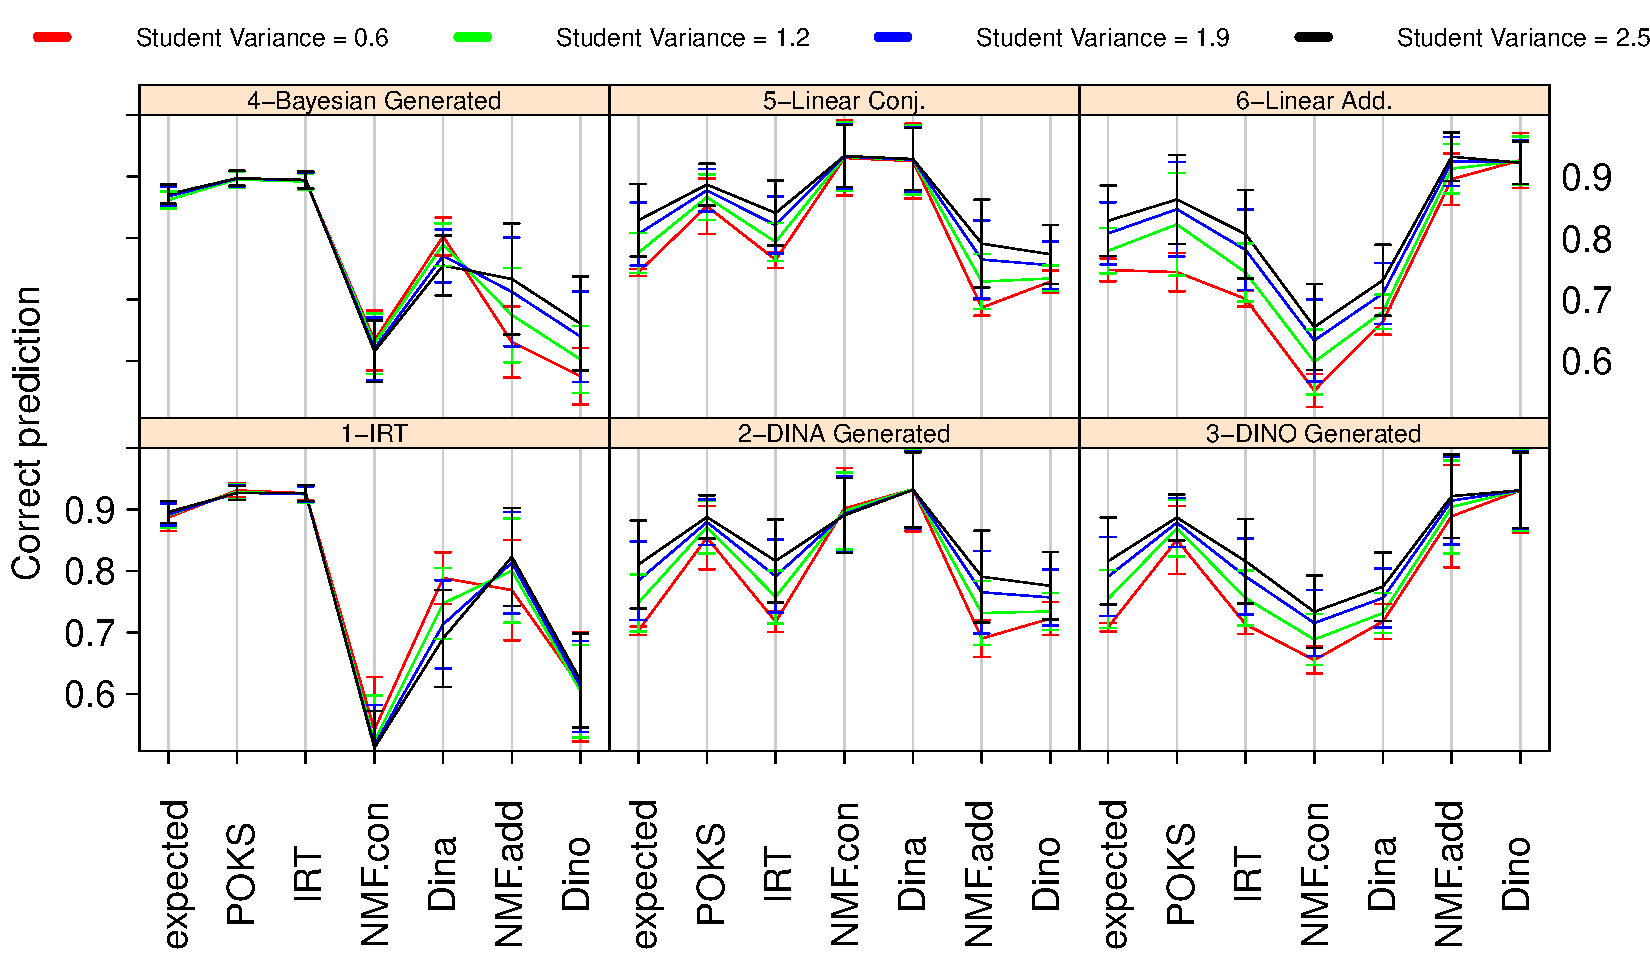
\includegraphics[scale=0.58]{StudentVariance.pdf}
\caption{Variation of \textbf{Student variance} Over synthetic data sets}
\label{figStudentVar}
\end{figure}


\begin{figure}
  \centering
    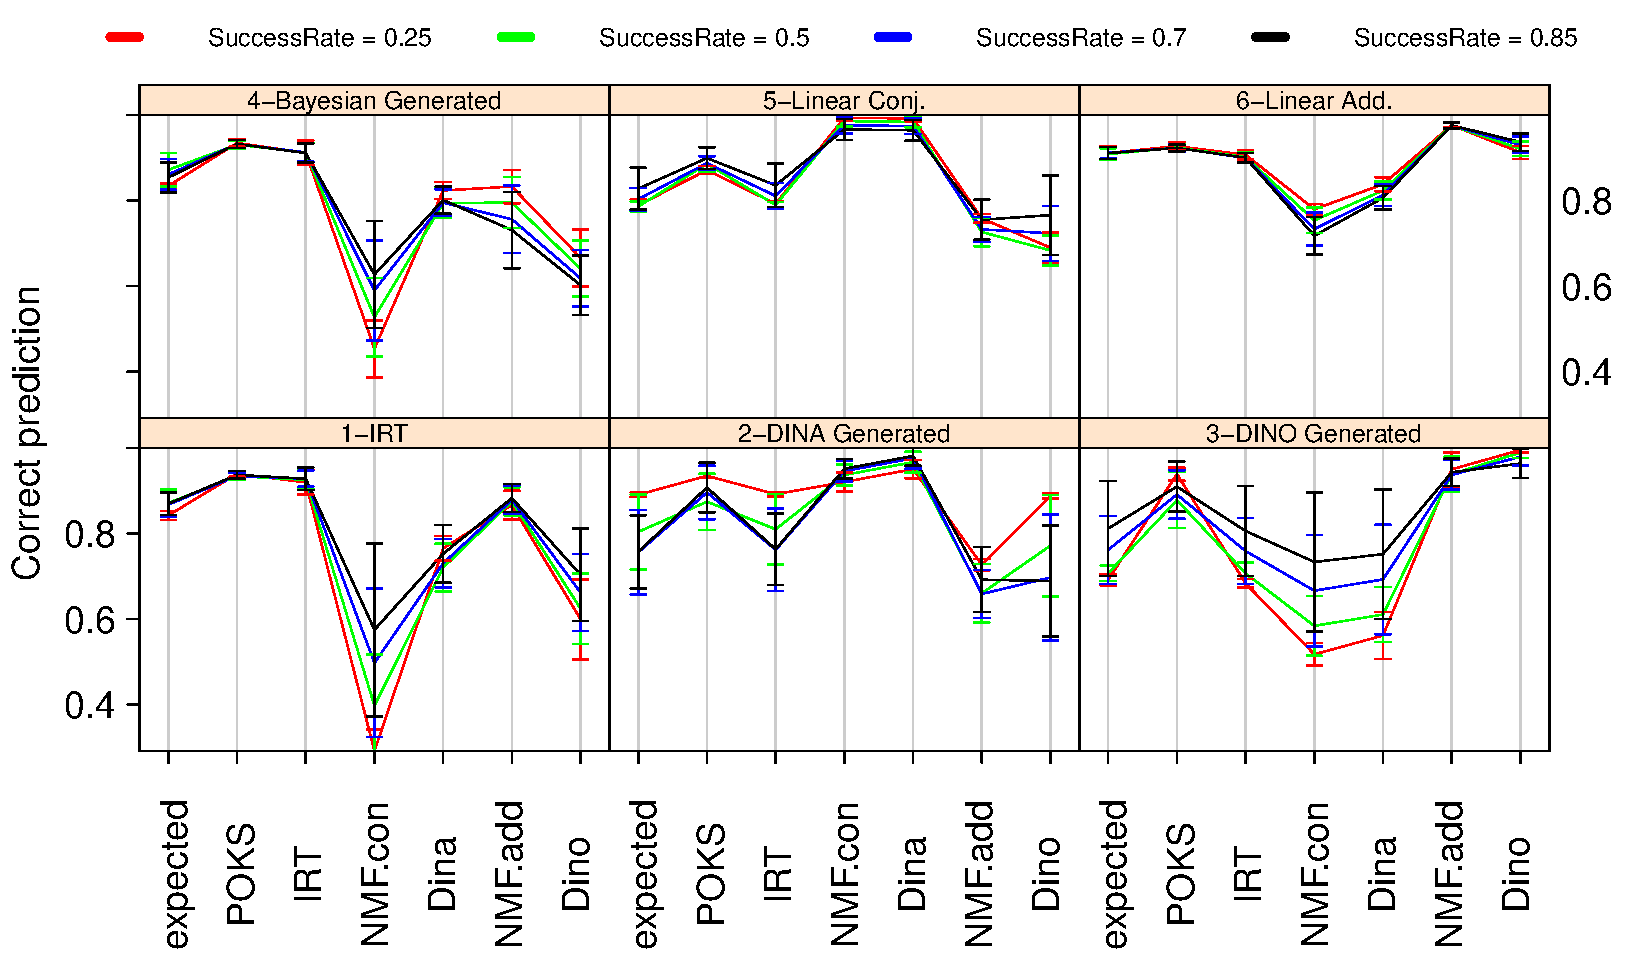
\includegraphics[scale=0.58]{Successrate.pdf}
\caption{Variation of \textbf{Success Rate} Over synthetic data sets}
\label{figSucceessRate}
\end{figure}


\subsection{Degree of similarity}
The most important part is to have a measure to show the degree of similarity between the model performance vector of the synthetic data and the one of the ground truth which is a measure of model fit in our study. Many measures can be used to calculate this degree. The simplest one can be finding the distance between two vector of predictive performance between the synthetic dataset and the real one. previous section showed that different data generation parameters with the same underlying model can create slightly different model performance vectors but with the same pattern. Using distance between each of these signatures with the same ground truth can possibly result in different values for similarity. In this research we used Pearson correlation coefficient as a measure of similarity.


The evaluation of this research consists of two parts. The first part is to measure the degree of similarity for synthetic vs. synthetic datasets. The second part is to identify the ground truth by measuring the correlation between real and synthetic datasets. 

Given $6\times 4$ different set of data generation parameters (described in section \ref{Sensitive}) and generating 10 times for each model will produce 1440 datasets. The comparison in our study is based on same data specific parameters. Therefore we can calculate the correlation table among 60 synthetic datasets that share same data specific parameters. This will result in 24 tables which consider all the possible data generation parameters. The expectation is that those vectors with same model show high correlation. Table~\ref{tablSyn} shows the average correlation of these 24  conditions.

Evaluating the synthetic dataset versus themselves can give a clue to how accurate this comparison is in model fitting. Basically, Those datasets that have the same model behind them should show a good correlation. The diagonal of table~\ref{tablSyn} shows a high correlation because it compares the same model generated datasets. On the other hand some models such as IRT and POKS shows a high correlation since they are not using multi-skills models. Those models that share concepts such as DINA and NMF conjunctive also resulted in a high correlation comparing with other models because they are linear models which deal with conjunctive model of Q-matrix. DINO and NMF additive has almost a high correlation but since the additive model is slightly different from the disjunctive model then it's less correlated.


\begin{table}
\center
\begin{tabular}{c|c|c|c|c|c|c|c|}
\multicolumn{2}{c}{} & \multicolumn{6}{c}{Synthetic Datasets} \tabularnewline
\multicolumn{8}{c}{} \tabularnewline
\cline{3-8} 
\multicolumn{2}{c|}{} & POKS & IRT & NMF Conj. & DINA & NMF Add. & DINO\tabularnewline
\cline{2-8}
\cline{2-3}
&POKS & \textbf {0.96} & \multicolumn{1}{|c}{} & \multicolumn{1}{c}{} & \multicolumn{1}{c}{} & \multicolumn{1}{c}{}\tabularnewline
\cline{2-4}
&IRT & 0.86 & \textbf {0.96} & \multicolumn{1}{|c}{} & \multicolumn{1}{c}{} & \multicolumn{1}{c}{} & \multicolumn{1}{c}{}\tabularnewline
\cline{2-5}
&NMF Conj. & 0.22 & -0.20 & \textbf {0.96} & \multicolumn{1}{|c}{} & \multicolumn{1}{c}{} & \multicolumn{1}{c}{}\tabularnewline
\cline{2-6}
&DINA & 0.02 & -0.40 & 0.94 & \textbf {0.96} & \multicolumn{1}{|c}{} & \multicolumn{1}{c}{}\tabularnewline
\cline{2-7}
&NMF Add. & 0.44 & 0.75 & -0.62 & -0.73 & \textbf {0.93} & \multicolumn{1}{|c}{}\tabularnewline
\cline{2-8}
\multicolumn{1}{c|}{\multirow{-6}{*}{\begin{sideways}Synthetic Datasets\end{sideways}}}&DINO & -0.15 & 0.20 & -0.70 & -0.69 & 0.63 & \textbf {0.95}\tabularnewline
\cline{2-8}
\end{tabular}
\caption{Degree of similarity between six synthetic datasets based on the correlation}
\label{tablSyn}
\end{table}



\begin{table}
 \center
\begin{tabular}{c|c|c|c|c|c|c|c|c|}

\multicolumn{2}{c}{}&\multicolumn{7}{c}{Real Datasets}\tabularnewline   
\multicolumn{9}{c}{}\tabularnewline   
\cline{6-9}
\multicolumn{5}{c|}{}&\multicolumn{4}{c|}{Fraction subsets}   \tabularnewline   
\cline{3-9} 
\multicolumn{2}{c|}{}   & Vomlel &ECPE &Fraction &1&21&22&23\tabularnewline
\cline{2-9}
\cline{2-9}
&Random & 0.58 &\textbf {0.73} & 0.61   & 0.43 & 0.24 & 0.61 & 0.57 \tabularnewline
\cline{2-9}
&IRT & \textbf {0.90} & 0.42 & 0.72   & 0.88 & 0.60 & 0.77 & 0.61 \tabularnewline
\cline{2-9}
&DINA & -0.38  & -0.09 &   0.23 &   0.30 & 0.56 & 0.06 & 0.38 \tabularnewline
\cline{2-9}
&DINO & 0.34 & 0.15  &  -0.18 &  -0.31 & 0.10 & -0.08 & 0.38 \tabularnewline
\cline{2-9}
&POKS & 0.75 &0.40  &  \textbf {0.83}  &  \textbf {0.95} &\textbf {0.70} & \textbf {0.83} & \textbf {0.80}\tabularnewline
\cline{2-9}
 &NMF Conj. & -0.05 & 0.54  & 0.51   & 0.55  & 0.66 & 0.33 & 0.57\tabularnewline
\cline{2-9}
\multicolumn{1}{c|}{\multirow{-7}{*}{\begin{sideways}Synthetic Datasets\end{sideways}}}&NMF Add. & 0.39 &0.06   & -0.04   & -0.19 & -0.03 & 0.13 & 0.28\tabularnewline
\cline{2-9}
\end{tabular}
\caption{Degree of similarity between six synthetic datasets and the ground truth based on the correlation}
\label{tablSynReal}
\end{table}


To assess a model fit for each real dataset with this approach we need to create datasets with described underlying models (7 techniques) which have the same parameters of data generation as the real data. Since some parameters influence the performance vector as described in the section~\ref{Sensitive} so we have to create synthetic data that follows the same characteristics of the real one. Table~\ref{tablSynReal} shows the correlation of real data signature in columns with the signature of synthetic data generated with underlying model in rows. Vomlel dataset shows a high correlation with IRT model and Fraction with its subset datasets show similarity with POKS model. As expected ECPE has the highest correlation with random generated dataset.







\begin{table}
\center
\begin{footnotesize}

\begin{adjustwidth}{-0.5cm}{}
\begin{tabular}{c|c!{\VRule[2pt]}c!{\VRule}c!{\VRule[2pt]}c|c!{\VRule[2pt]}c|c!{\VRule[2pt]}c|c!{\VRule[2pt]}c|c!{\VRule[2pt]}c|c!{\VRule[2pt]}c|c|}
\multicolumn{3}{c}{ BP: Best Performer}&\multicolumn{11}{c}{Datasets}&\multicolumn{2}{c}{}\tabularnewline
\cline{15-16}
\multicolumn{3}{c}{ NN: Nearest Neighbor}&\multicolumn{11}{c!{\VRule[2pt]}}{}& \multicolumn{2}{|c|}{Accuracy} \tabularnewline
\cline{3-14}
\multicolumn{2}{c|}{}&\multicolumn{2}{c|}{ POKS}&\multicolumn{2}{c|}{ IRT}&\multicolumn{2}{c|}{ NMF Conj.}&\multicolumn{2}{c|}{ DINA}&\multicolumn{2}{c|}{ NMF Add}&\multicolumn{2}{c!{\VRule[2pt]}}{ DINO}&\multicolumn{2}{c|}{  \scriptsize (\%)}\tabularnewline
\cline{3-16}
\multicolumn{1}{c}{}&\multicolumn{1}{c|}{}&\multicolumn{1}{c|}{ BP}&\multicolumn{1}{c|}{ NN}&\multicolumn{1}{c|}{ BP}&\multicolumn{1}{c|}{ NN}&\multicolumn{1}{c|}{ BP}&\multicolumn{1}{c|}{ NN}&\multicolumn{1}{c|}{ BP}&\multicolumn{1}{c|}{ NN}&\multicolumn{1}{c|}{ BP}&\multicolumn{1}{c|}{ NN}&\multicolumn{1}{c|}{ BP}&\multicolumn{1}{c!{\VRule[2pt]}}{ NN}&\multicolumn{1}{c|}{ BP}&\multicolumn{1}{c|}{ NN}\tabularnewline
\cline{3-16}
\cline{3-16}
\cline{2-16}
\multicolumn{1}{c|}{}& Expected& 0& 0& 0& 0& 0& 0& 0& 0&12& 0& 2& 0& & \tabularnewline
\cline{2-16}
\multicolumn{1}{c|}{}& POKS&\cellcolor{gray!25} 238&\cellcolor{gray!25} 218&130&32&21& 12&14& 0&18&13& 1& 0&85&95\tabularnewline
\cline{2-16}
\multicolumn{1}{c|}{}& IRT& 2& 20&\cellcolor{gray!25}110&\cellcolor{gray!25}208& 0& 0& 0& 0& 0&15& 0& 3&100&97\tabularnewline
\cline{2-16}
\multicolumn{1}{c|}{}& NMF \scriptsize Conj.& 0& 0& 0& 0&\cellcolor{gray!25}82&\cellcolor{gray!25}180& 5&73& 0& 0& 0& 0&100&94\tabularnewline
\cline{2-16}
\multicolumn{1}{c|}{}& DINA& 0& 0& 0& 0&137&48&\cellcolor{gray!25}221&\cellcolor{gray!25}167& 0& 0& 0& 0&87&96\tabularnewline
\cline{2-16}
\multicolumn{1}{c|}{}& NMF \scriptsize Add.& 0& 2& 0& 0& 0& 0& 0& 0&\cellcolor{gray!25}210&\cellcolor{gray!25}211& 14&10&99&99\tabularnewline
\cline{2-16}
\multicolumn{1}{c|}{\multirow{-7}{*}{\begin{sideways}Models\end{sideways}}}& DINO& 0& 0& 0& 0& 0& 0& 0& 0& 0& 1&\cellcolor{gray!25}223&\cellcolor{gray!25}227&100&100\tabularnewline
\cline{1-16}
\multicolumn{2}{|c!{\VRule[2pt]}}{ Accuracy \scriptsize (\%)} & 99 & 91 & 46 & 87 &34 & 75 & 92 & 70 & 88 & 87 & 93 & 95&\multicolumn{2}{|c}{}\tabularnewline
\cline{1-14}
\end{tabular}
\end{adjustwidth}

\end{footnotesize}

\caption{Confusion matrix for classification of 210 synthetic datasets on 7 models with Best performer Vs. Nearest neighbor methods}
\label{Classification-Conf}
\end{table}










\begin{table}
\center	
%\begin{scriptsize}
\begin{tabular}{c|c|c|c|c|c!{\VRule[2pt]}c|c|c|c|}
\multicolumn{2}{c}{}&\multicolumn{8}{c}{Performance}\tabularnewline
\cline{3-10}
\multicolumn{2}{c|}{}&\multicolumn{4}{c|}{Best Performer}&\multicolumn{4}{c|}{Nearest Neighbor}\tabularnewline
\cline{3-10}
\multicolumn{2}{c|}{}&\scriptsize Precision&\scriptsize Recall&\multicolumn{1}{c|}{\scriptsize F-Measure}&\scriptsize Accuracy&\scriptsize Precision&\scriptsize Recall&\scriptsize F-Measure&\scriptsize Accuracy\tabularnewline
\cline{2-10}
&POKS&0.564&0.992&0.719&0.871&0.793&0.908&\cellcolor{gray!25}0.847&\cellcolor{gray!25}0.945\tabularnewline
\cline{2-10}
&IRT&0.982&0.458&0.625&0.908&0.846&0.867&\cellcolor{gray!25}0.856&\cellcolor{gray!25}0.951\tabularnewline
\cline{2-10}
&NMF Conj.&0.943&0.342&0.502&0.887&0.711&0.750&\cellcolor{gray!25}0.730&\cellcolor{gray!25}0.907\tabularnewline
\cline{2-10}
&DINA&0.617&0.921&0.739&0.891&0.777&0.696&\cellcolor{gray!25}0.734&\cellcolor{gray!25}0.916\tabularnewline
\cline{2-10}
&NMF Add.&0.938&0.875&0.905&0.969&0.946&0.879&\cellcolor{gray!25}0.911&\cellcolor{gray!25}0.971\tabularnewline
\cline{2-10}
\multicolumn{1}{c|}{\multirow{-7}{*}{\begin{sideways}Models\end{sideways}}}&DINO&1&0.929&\cellcolor{gray!25}0.963&\cellcolor{gray!25}0.988&0.996&0.946&\cellcolor{gray!25}0.970&\cellcolor{gray!25}0.990\tabularnewline
\cline{2-10}
\end{tabular}
\caption{Accuracy of best performer and nearest neighbor classification methods  }
\label{Classification-Acc}
\end{table}
The very last experiment that we have done is a comparison between the proposed approach where the nearest neighbor classifies in the performance vector space and the simplest approach where the best performer is defining the ground truth. The process is straightforward which is preforming a classification for all synthetic data with best performer method. For the nearest neighbor approach the classification should be done where datasets have the same data generation conditions. Therefore we'll get 24 sets of datasets where similar dara generation parameters exists among each set.Since we have 10 runs for each data specific parameter set then we choose 10 nearest neighbor and preform majority voting on the classification results.

 Table~\ref{Classification-Conf} shows the confusion matrix of this experiment. There exists 1440~datasets where each model corresponds to 240 dataset. The gray cells in table~\ref{Classification-Conf} shows the true positive values and other values in each column represent the false positive predictions for group of datasets.The values in each row shows the number of false negative predictions for each model. The confusion is mostly between those techniques that shares same concepts specially between NMF Conjunctive and DINA model where we use conjunctive Q-matrices. 

The accuracy that is reported in the last row of table~\ref{Classification-Conf} is calculated based on $\frac{TP}{240}$ which counts the true positive predictions for each sub set of datasets that have the same model behind them. The accuracy the is reported in the last two columns of table~\ref{Classification-Conf} is considering how faithful the classification is to select a dataset that doesn't have the related model behind it which will count true negative values based on $\frac{TN}{1200}$ (1200 is the number of datasets that do not have same underlaying models). In terms of true positive selections there is no benefit between any of these methods even if sometimes best performer shows to be better (specially for DINA and IRT).

Considering the false negative and false positive changes the classification results. Table~\ref{Classification-Acc} shows the accuracy of this classification in terms of precision, recall, $F1$ measure and accuracy ($\frac{TN+TP}{1440}$). Since $F1$ measure is combining both precision and recall, then it is a good measure for improvement. The third column of each classification method shows that F-measure increased for Nearest neighbor method which is almost close to $1$. Also in terms of individual scores per method we also report accuracy of each technique which considers true positive and true negative values. The last column of table~\ref{Classification-Acc} shows this improvement. The total accuracy which is considering true positive numbers over number of datasets regardless of individual models shows that best performer  gets $0.75\%$ and the nearest neighbor gets upto $0.84\%$ of accuracy.



%\include{7-Theme1}             % Premier thème (Doctorat) ou "Détails de la Solution" (Maîtrise).
%\include{7-Theme2}             % Second thème (Doctorat) ou "Résultats théoriques et expérimentaux" (Maîtrise).
%\include{7-Theme3}             % Troisième thème (Doctorat) ou effacez ce fichier si vous êtes à la Maîtrise.
\Chapter{Conclusion and future work}\label{sec:Conclusion}

In this thesis, the performance of seven student skills assessment models is assessed and used to define a framework for evaluating mode fit.  Model fit of a data set is defined as the similarity between the \textit{performance vector} obtained over this data set and, the \textit{performance prototype} vectors obtained over synthetic data sets.

Let us return to the conjecture that the comparison of performance vectors over synthetic data can help determine whether a specific skill model corresponds to the ground truth of some data set. As described, the standard practice is to select the model that has the highest predictive performance as the best fit.  Using synthetic data, we have shown that the generative model does not always correspond to the best performer, and that an approach based on defining a vector space model of performance and on finding the nearest synthetic data point to the target data in that space provides a more reliable means to find the underlying model behind the target data.

This means of determining a data set's ground truth is made possible because the synthetic data sets have very distinct performance patterns, showing sharp differences across models.  The data sets from a single model tend to share a strong similarity among themselves, and show strong dissimilarity from most other models.  This property of synthetic \textit{performance vectors} cluster around distinct \textit{performance prototypes} is very strong for synthetic data.

Another finding is that we find evidence that data sets that share a common source have correlated \textit{performance vectors}.  This happens with the Fraction data sets.  They all have a similar pattern of performances across different subsets of items, different number of skills (latent factors), and different variants of the models as expressed by variations in the Q-matrices. Only when the Q-matrix has a very different property, namely a single skill per item, we do observe a different \textit{performance vector} for the models that depend on the Q-matrix (NMF conjunctive, DINA, NMF additive, and DINO).  

However, the similarity of \textit{performance vectors} does not seem to substantially extend to data that shares the same domain: although the Vomlel data is within the same domain as the Fraction data, namely arithmetic, the performance signatures are relatively different between the two.  This could be attributed to the Q-matrices involved (although both are multiple skills and therefore the difference is not due to the formal property of single skill per item), but other factors could also be involved such as sensitivity to data specific parameters.

The other interesting finding is that for real data sets the performances are not better than the expected performance and the conclusion behind that can be either the ground truth is not among the candidate models, or the best performer is not necessarily the ground truth. 



The highest correlation was for Vomlel dataset, which selects IRT as the ground truth. As expected, for the ECPE data set, the \textit{performance vector} is close to that of random data which resulted in very small differences among model performances. Note that this dataset comes from English examination domain and our investigation shows that a simple query among records retrieves all possible combination of test results, which is an evidence of randomness.

The results of assessing model fit for synthetic data show that some datasets with different ground truths that share some concepts, show a high correlation. For example, datasets based on linear conjunctive and DINA model. There exist no correlation for those that have completely different underlying models.

Furthermore investigations show that the predictive performance of each model over a dataset is dependent to different model and data specific parameters. For some parameters the \textit{performance vector} stays stable but some others play an important role in changing this vector. Although the predictive \textit{performance vector} changes for some parameters but it still shows a high correlation with datasets with the same ground truth.


The most important finding of this research is that the best performer may not be the model that is most representative of the ground truth, but instead it may be the result of contextual factors that make this model outperform the ground truth one. The last experiment tests the accuracy of signature approach versus best performer to classify a set of synthetic datasets with different contextual parameters. The results confirm that the ``signature'' approach shows a better accuracy in terms of measures for the confusion table in the span of different parameter conditions. This also shows the effect of data generation parameters on the best performer and reliability of these approaches on different assumptions about the data.

\section{Limits}

\note{I meant here to write a text in normal form, not in short bullet sentences.}

  \begin{enumerate}
  \item This study limits to static data opposed to dynamic data. Dynamic skill assessment models such as BKT are very important in EDM.  
  \item This research is also limited mostly to fraction data where students skill assessment in other domains has the same importance.%limit on generalization
  \item Most of our findings were through experiments over synthetic data. Although synthetic data is widely used to validate research results but it does not have the complexity of the real world.%: generality of the findings
  \item We test this approach with 7 models but still the number of candidate models and their complexity could be an important factor. %dependent on the models; would it work if we only had 2 models?
  \end{enumerate}

\section{Future Work}

Further studies with real and simulated data are clearly needed.  For example, there are other real datasets that potentially require a different set of candidate models. And this requires new approaches to generate synthetic data with respect to these skills assessment models.

However, the approach would generalize to dynamic data as well. This approach is using static models to assess a model fit but dynamic models are also used widely in EDM. This contribution also requires data generation and performance assessment of each model.

In this thesis we compared the ``signature'' approach with the ``best performer'' in terms of ground truth classification on synthetic data. The potential future contribution would be preparing a survey on different model selection approaches with their error metrics such as likelihood and comparing their performance over synthetic data.

One important future work is to give different weights to different parts of the space to justify the performance gain where in our research we assumed that the space is equally important.

Finally, because selecting right model is an important factor in all fields of studies, this approach could be applied in general fields as well. EDM is the example that we applied in our research but it can be tested in other fields of studies.
         % Conclusion.
%\backmatter
\renewcommand\bibname{References}
\bibliography{Document}
%\bibliographystyle{polymtl}  % Format de la bibliographie.
\bibliographystyle{IEEEtranSN-francais}  % Format de la bibliographie.
%
%\ifthenelse{\equal{\AnnexesPresentes}{O}}{
%\appendix%
%\newcommand{\Annexe}[1]{\annexe{#1}\setcounter{figure}{0}\setcounter{table}{0}\setcounter{footnote}{0}}%
%%%
%%  Annexes.
%%
%%  Note: Ne pas modifier la ligne ci-dessous.
\addcontentsline{toc}{compteur}{ANNEXES}
%%
%%
%%  Toutes les annexes doivent être inclues dans ce document
%%  les unes à la suite des autres.
\Annexe{DÉMO}
Texte de l'annexe A\@. Remarquez que la phrase précédente se termine
par une lettre majuscule suivie d'un point. On indique explicitement
cette situation à \LaTeX{} afin que ce dernier ajuste correctement
l'espacement entre le point final de la phrase et le début de la
phrase suivante.


\begin{landscape}
\Annexe{ENCORE UNE ANNEXE}
Texte de l'annexe B\@ en mode «landscape».
\end{landscape}

\Annexe{UNE DERNIÈRE ANNEXE}
Texte de l'annexe C\@.
}{}
\end{document}
